%----------------------------------------------------------------------------------------
%	CHAPTER 2 Teoría Clasica de Campos
%----------------------------------------------------------------------------------------

\chapterimage{chapter_head_1.pdf}  
% Chapter heading image


\chapter{Teor\'{\i}a Cl\'{a}sica de Campos} \label{capitulo_22}


Antes de tratar la cuantización de campos, se repasara primero el principio básico 
de la mecánica clásica para un sistema de $N$ partículas en el formalismo lagrangiano. Además se tratarán 
algunas de las t\'{e}cnicas b\'{a}sicas involucradas en la formulaci\'{o}n covariante de la teor\'{\i}a cl\'{a}sica de campos.

\section{Mecánica de partículas}

\subsection{Principio de acción y ecuaciones de Euler-Lagrange}
\vspace{0.1cm}
Todas las teor\'{\i}as de la f\'{\i}sica cl\'{a}sica pueden describirse partiendo del principio de m\'{\i}nima acci\'{o}n. Al considerar un sistema no relativista de $N$ partículas, se tiene que este sistema presenta $3N$ grados de libertad descritos por un conjunto de coordenadas $q(\mathbf{x},t)$ que, junto con sus derivadas temporales $\dot{q}(\mathbf{x},t)$, describen adecuadamente la configuraci\'{o}n y evoluci\'{o}n del sistema en el espacio de configuraciones. Se puede utilizar el conocimiento de las simetr\'{\i}as\footnote{Ver apéndice \ref{A1}} del sistema para reducir este conjunto al menor n\'{u}mero de coordenadas independientes. Por otro lado, en casi todos los casos interesantes es \'{u}til no hacer la reducci\'{o}n sino elegir un conjunto de coordenadas que tengan interrelaciones simples, haciendo expl\'{\i}citas las simetr\'{\i}as del sistema.\\

Ahora se definen dos objetos matem\'{a}ticos que ser\'{a}n de gran utilidag para el desarrollo del curso.\\


Se identifica a $L$ como el \textbf{Lagrangiano} del sistema, siendo una función de las coordenadas $q_{i}$ y sus derivadas temporales $\dot{q}_{i}$, es decir $L=L(q,\dot{q})$. Generalmente,
\begin{equation}
    L(q,\dot{q})=\sum_{i} \frac{1}{2}m_{i}\dot{q}_{i}^{2}-V(q)~~~~~~~~~\text{(Término cinético menos el potencial)}.
\end{equation}

%Supondremos que el sistema es conservativo, de modo que el lagrangiano no depende explicitamente del tiempo. 
Se introduce la \textbf{acci\'{o}n} $S$, definida como

\begin{equation}
S=\int_{t_{1}}^{t_{2}}dt\ L\left( q_{i},\dot{q}_{i},t\right),
\label{2.1}
\end{equation}

donde $t_{1}$ y $t_{2}$ son los tiempos inicial y final entre los cuales se est\'{a} estudiando la evoluci\'{o}n del sistema. Cabe resaltar que si existe una fuente o sumidero de energ\'{\i}a en el sistema en consideraci\'{o}n, el lagrangiano tambi\'{e}n puede depender expl\'{\i}citamente del tiempo.\\

El \emph{principio de m\'{\i}nima acci\'{o}n} establece que, entre todas las trayectorias que unen las coordenadas de un estado inicial fijo $q_{i}(t_{1})$ con otro final $q_{i}(t_{2})$ (ver figura \ref{mA}), la trayectoria real que adquiere el sistema 
es aquella que cumple que $S$ sea estacionario (generalmente un mínimo).\\

\begin{figure}[h!]
    \centering
    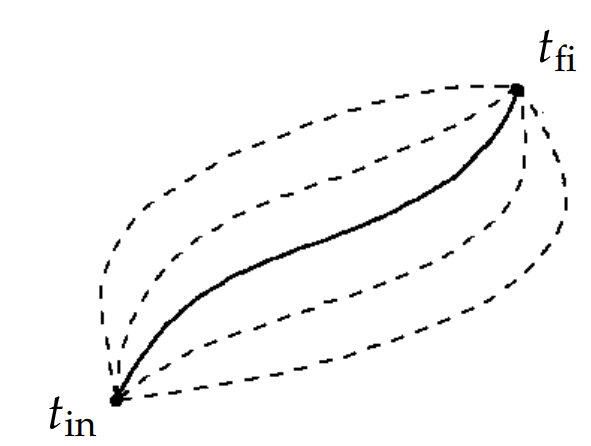
\includegraphics[scale=0.25]{Capitulos/Cap_2/minacc.png}
    \caption{Posibles caminos $q_{i}(t)$ que puede seguir un sistema en el espacio de las coordenadas
entre un instante inicial $t_{1}$ y otro final $t_{2}$.}
    \label{mA}
\end{figure}

Para ver lo que esto implica, considere variaciones infinitesimales alrededor de una trayectoria definida por $q_{i}(\mathbf{r},t)$ y $\dot{q}_{i}(\mathbf{r},t)$,

\begin{eqnarray}
q_{i}(\mathbf{r},t) &\rightarrow &q_{i}(\mathbf{r},t)+\delta q_{i}(\mathbf{r},t)  \label{2.2} \\
\dot{q}_{i}(\mathbf{r},t) &\rightarrow &\dot{q}_{i}(\mathbf{r},t)+\delta 
\dot{q}_{i}(\mathbf{r},t)~~~~~.  \label{2.2a}
\end{eqnarray}

Esto introduce la siguiente variaci\'{o}n de la acci\'{o}n definida en la
ecuaci\'{o}n (\ref{2.1}),

\begin{eqnarray}
\delta S &=&\delta \int_{t_{1}}^{t_{2}}dt\ L\left( q_{i},\dot{q}%
_{i},t\right) =\int_{t_{1}}^{t_{2}}dt\ \left( \frac{\partial L}{\partial
q_{i}}\delta q_{i}+\frac{\partial L}{\partial \dot{q}_{i}}\delta \dot{q}%
_{i}\right)   \notag \\
&=&\int_{t_{1}}^{t_{2}}dt\ \left( \frac{\partial L}{\partial q_{i}}\delta
q_{i}+\frac{\partial L}{\partial \dot{q}_{i}} \frac{d}{dt}\delta q_{i} \right)
,  \label{2.3}
\end{eqnarray}
aquí se ha considerado que:
\begin{equation}
\delta \dot{q}_{i}=\frac{\partial \dot{q}_{i}}{\partial \alpha} \delta \alpha=\frac{\partial}{\partial \alpha}\left(\frac{\mathrm{d} q_{i}}{\mathrm{~d} t}\right) \delta \alpha=\frac{\mathrm{d}}{\mathrm{d} t}\left(\frac{\partial q_{i}}{\partial \alpha}\right) \delta \alpha=\frac{\mathrm{d}}{\mathrm{d} t} \delta q_{i}~,
\end{equation}
siendo $\alpha$ un conjunto discreto de parámetros tal que $q_{i}= q_{i}(\alpha,t)$ es lo suficientemente suave de modo que las derivadas respecto a $\alpha$ y respecto a $t$ conmutan, de modo que es posible discretizar ambas variaciones. También se ha utilizado la convenci\'{o}n de suma para el \'{\i}ndice $i$. Suponiendo que el sistema es conservativo, el lagrangiano que describe el sistema no tiene ninguna dependencia temporal expl\'{\i}cita. Entonces al integrar por partes resulta,

\begin{equation}
\delta S=\left. \frac{\partial L}{\partial \dot{q}_{i}}\delta
q_{i}\right\vert _{t_{1}}^{t_{2}}+\int_{t_{1}}^{t_{2}}dt\ \left[ \frac{%
\partial L}{\partial q_{i}}-\frac{d}{dt}\left( \frac{\partial L}{\partial 
\dot{q}_{i}}\right) \right] \delta q_{i}  \label{2.3a}.
\end{equation}

\begin{exercise}
Demostrar aplicando integraci\'{o}n por partes, que se cumple la relaci\'{o}%
n (\ref{2.3a})
\end{exercise}

\begin{solution}
Para llegar a la expresi\'{o}n (\ref{2.3a}), se considera la integral 
\begin{equation}
\int_{t_{1}}^{t_{2}}dt\ \frac{\partial L}{\partial \dot{q}_{i}} \frac{d}{dt} \delta q_{i}  \label{2.3b}
\end{equation}%
aplicando integraci\'{o}n por partes $\int_{a}^{b}udv=\left. uv\right\vert
_{a}^{b}-\int_{a}^{b}vdu$, entonces se requiere definir 
\begin{equation*}
u=\frac{\partial L}{\partial \dot{q}_{i}}~\ \ \ \ ,~~~dv=dt\ \frac{d}{dt} \delta q_{i} \quad \ ,~~\ \ du=\frac{d}{dt}\left( \frac{\partial L}{\partial 
\dot{q}_{i}}\right) dt~.
\end{equation*}%
de aqu\'{\i} se obtiene 
\begin{equation*}
v=\int dt\ \frac{d\left( \delta
q_{i}\right) }{dt}=\delta q_{i}~~\impliedby \text{Variaciones sobre las
coordenadas y no sobre $t$}
\end{equation*}%
de manera que en (\ref{2.3b}),
\begin{equation}
\int_{t_{1}}^{t_{2}}dt\ \frac{\partial L}{\partial \dot{q}_{i}} \frac{d}{dt}\delta q_{i}=\left. \left( \frac{\partial L}{\partial \dot{q}_{i}}\delta
q_{i}\right) \right\vert _{t_{1}}^{t_{2}}-\int_{t_{1}}^{t_{2}}dt\ \delta
q_{i}\frac{d}{dt}\left( \frac{\partial L}{\partial \dot{q}_{i}}\right).
\label{2.3c}
\end{equation}%

Reemplazando (\ref{2.3c}) en la integral (\ref{2.3}):%
\begin{eqnarray}
\delta S &=&\int_{t_{1}}^{t_{2}}dt\ \frac{\partial L}{\partial q_{i}}\delta
q_{i}+\int_{t_{1}}^{t_{2}}dt\frac{\partial L}{\partial \dot{q}_{i}}\frac{d}{dt}\delta q_{i} \notag\label{2.4a} \\
&=&\int_{t_{1}}^{t_{2}}dt\ \frac{\partial L}{\partial q_{i}}\delta
q_{i}+\left. \frac{\partial L}{\partial \dot{q}_{i}}\delta q_{i}\right\vert
_{t_{1}}^{t_{2}}-\int_{t_{1}}^{t_{2}}dt\ \delta q_{i}\frac{d}{dt}\left( 
\frac{\partial L}{\partial \dot{q}_{i}}\right)   \notag \\
&\therefore &~\delta S=\left. \frac{\partial L}{\partial \dot{q}_{i}}\delta
q_{i}\right\vert _{t_{1}}^{t_{2}}+\int_{t_{1}}^{t_{2}}dt\ \left[ \frac{%
\partial L}{\partial q_{i}}-\frac{d}{dt}\left( \frac{\partial L}{\partial 
\dot{q}_{i}}\right) \right] \delta q_{i}~.  \label{2.4}
\end{eqnarray}

\end{solution}

Dado que se están buscando caminos que conectan las configuraciones inicial y final $q_{i}(t_{1})$ y $q_{i}(t_{2})$, no se variar\'{a}n los puntos
finales. As\'{\i}, entonces se establece que los puntos extremos estén fijos de manera que
\begin{equation}
\delta q_{i}(t_{1})=\delta q_{i}(t_{2})=0~,  \label{2.5}
\end{equation}

conllevando a que el primer t\'{e}rmino de la ecuaci\'{o}n (\ref{2.4}) desaparezca. El principio de m\'{\i}nima acci\'{o}n establece que, cerca del camino cl\'{a}sico, la variaci\'{o}n de la acci\'{o}n debe ser cero. Esto es cierto para cualquier variaci\'{o}n virtual arbitraria, es decir, para 
cualquier $\delta q_{i}(t)$, entonces, $\delta S=0$ ocurre si,

\begin{equation}
\frac{\partial L}{\partial q_{i}}-\frac{d}{dt}\left( \frac{\partial L}{%
\partial \dot{q}_{i}}\right) =0~, ~~~~~~~~\text{(Ecuaciones de Euler-Lagrange)}   \label{2.6}
\end{equation}

\vspace{0.1cm}
donde se ha puesto de manifiesto el teorema fundamental del calculo variacional. A (\ref{2.6}) se las conoce en la literatura como las
ecuaciones de movimiento de Euler-Lagrange, correspondientes a las coordenadas $q_{i}$.\\


\begin{exercise}
Encontrar la ecuaci\'{o}n de movimiento descrita por una part\'{\i}cula de
masa $m$ que se mueve bajo la influencia de un potencial $V\left( x\right) $
independiente del tiempo.\\
\end{exercise}
\begin{solution}
Para una part\'{\i}cula de masa $m$ que se mueve en un potencial $V(x)$
independiente del tiempo, una opci\'{o}n conveniente y que usualmente se usa
para el lagrangiano es:%
\begin{equation*}
L=T-V
\end{equation*}%
\begin{equation}
L=\frac{1}{2}m\dot{x}^{2}-V\left( x\right) ~.  \label{2.7}
\end{equation}%
Entonces la ecuaci\'{o}n de Euler-Lagrange derivada de este lagrangiano es:%
\begin{equation*}
\frac{\partial L}{\partial x}=\frac{dV\left( x\right) }{dx}~\ \ \ \ ;~\ \ \
\ \frac{\partial L}{\partial \dot{x}}=m\dot{x}
\end{equation*}%
\begin{equation*}
\frac{d}{dt}\left( \frac{\partial L}{\partial \dot{q}_{i}}\right) =m\ddot{x}~,
\end{equation*}%
de ahi que en (\ref{2.6}) se obtenga%
\begin{equation}
m\ddot{x}=\frac{dV\left( x\right) }{dx}~,  \label{2.8}
\end{equation}%
que se conoce com\'{u}nmente como \emph{la segunda ley de Newton} de
movimiento.
\end{solution}

\subsection{Formalismo Hamiltoniano y corchetes de Poisson}

La parte independiente de la velocidad del Lagrangiano se puede considerar
como energ\'{\i}a potencial generalizada. As\'{\i} que, se puede hacer que
las ecuaciones de Euler-Lagrange se vean como la segunda ley de Newton
definiendo los \emph{momentos can\'{o}nicos conjugados} generalizados
asociados a la coordenada $q_{i}$\ como:

\begin{equation}
p_{i}=\frac{\partial L(q_{i},\dot{q}_{i})}{\partial \dot{q}_{i}}~.
\label{2.9}
\end{equation}

Habr\'{a} una de estas ecuaciones para cada valor del \'{\i}ndice $i$,
siempre y cuando el sistema a tratar sea regular. Dado que el Lagrangiano es
una funci\'{o}n de las posiciones y las velocidades, los lados derechos de
estas ecuaciones son, en general, funciones de las $q^{\prime }s$ y las $%
\dot{q}^{\prime }s$. Suponer que estas ecuaciones son invertibles, es decir,
las $\dot{q}^{\prime }s$ pueden resolverse en t\'{e}rminos de las posiciones
y los momentos, esto es posible siempre que el determinante de la matriz
Hessiana sea diferente de cero.

Entonces se introduce el Hamiltoniano escrito en t\'{e}rminos de las nuevas
variables $(q,p),$ el cual resulta de aplicar una transformaci\'{o}n de
Legendre al lagrangiano, de este modo:\bigskip 

\begin{equation}
H\left( q,p\right) =p_{i}\dot{q}_{i}\left( q,p\right) -L\left( q,\dot{q}%
\left( q,p\right) \right) ~.  \label{2.10}
\end{equation}

Sin embargo, por diferenciaci\'{o}n se tiene

\begin{eqnarray}
dH &=&p_{i}d\dot{q}_{i}+\dot{q}_{i}dp_{i}-dL\left( q,\dot{q}\right) 
\label{2.11} \\
&=&p_{i}d\dot{q}_{i}+\dot{q}_{i}dp_{i}-\left( \frac{\partial L}{\partial
q_{i}}dq_{i}+\frac{\partial L}{\partial \dot{q}_{i}}d\dot{q}_{i}\right)  
\notag \\
&=&p_{i}d\dot{q}_{i}+\dot{q}_{i}dp_{i}-\frac{\partial L}{\partial q_{i}}%
dq_{i}-p_{i}d\dot{q}_{i}~.  \label{2.11a}
\end{eqnarray}

Los t\'{e}rminos con $d\dot{q}_{i}$ se cancelan entre s\'{\i} debido a la definici\'{o}n de momento can\'{o}nico conjugado en la ecuaci\'{o}n (2.9). El t\'{e}rmino con $dq_{i}$ se puede simplificar mediante el uso de la ecuaci\'{o}n de Euler-Lagrange y la ecuaci\'{o}n (\ref{2.9}), para que finalmente se pueda escribir

\begin{eqnarray*}
p_{i} &=&\frac{\partial L(q_{i},\dot{q}_{i})}{\partial \dot{q}_{i}}~\ \implies ~\frac{d}{dt}p_{i}=\frac{d}{dt}\left[ \frac{\partial L(q_{i},\dot{q}_{i})}{\partial \dot{q}_{i}}\right] =\frac{\partial L}{\partial q_{i}} \\
&\therefore &~\ \dot{p}_{i}=\frac{\partial L}{\partial q_{i}}~,
\end{eqnarray*}

\bigskip de manera que en (\ref{2.11a}),

\begin{equation}
dH=\dot{q}_{i}dp_{i}-\dot{p}_{i}dq_{i}~.  \label{2.12}
\end{equation}%
confirmando el hecho de que el hamiltoniano es de hecho una funci\'{o}n de
las posiciones y los momentos. Adem\'{a}s, conduce directamente a las
ecuaciones de movimiento de Hamilton:

\begin{equation}
\dot{q}_{i}=\frac{\partial H}{\partial p_{i}}~\ \ \ ~\ ,\qquad \dot{p}_{i}=-%
\frac{\partial H}{\partial q_{i}}~.  \label{2.13}
\end{equation}

\bigskip

Por otro lado, el corchete de Poisson de dos variables din\'{a}micas
cualesquiera se define de la siguiente manera:

\begin{equation}
\left\{ f_{1},f_{2}\right\} =\frac{\partial f_{1}}{\partial q_{i}}\frac{%
\partial f_{2}}{\partial p_{i}}-\frac{\partial f_{1}}{\partial p_{i}}\frac{%
\partial f_{2}}{\partial q_{i}}~,  \label{2.14}
\end{equation}

\noindent
bajo esta definici\'{o}n, es trivial verificar que

\begin{eqnarray*}
\left\{ q_{i},p_{j}\right\}  &=&\frac{\partial q_{i}}{\partial q_{k}}\frac{%
\partial p_{j}}{\partial p_{k}}-\frac{\partial q_{i}}{\partial p_{k}}\frac{%
\partial p_{j}}{\partial q_{k}}=\delta _{ik}\delta _{jk} \\
&=&\delta _{ij}~,
\end{eqnarray*}

%es decir

%\begin{equation}
%\left\{ q_{i},p_{j}\right\} =\delta _{ij}~~~~~,  \label{2.15}
%\end{equation}

\noindent
y que las ecuaciones de Hamilton se pueden reescribir como:

\begin{equation}
\dot{q}_{i}=\left\{ q_{i},H\right\} \qquad~~;~~ \qquad \dot{p}_{i}=\left\{ p_{i},H\right\} _{p}~.  \label{2.16}
\end{equation}

M\'{a}s generalmente, si $f$ es una variable din\'{a}mica, su evoluci\'{o}n temporal se puede escribir en t\'{e}rminos el par\'{e}ntesis de Poisson como

\begin{equation}
\dot{f}\equiv \frac{df}{dt}=\frac{\partial f}{\partial t}+\left\{f,H\right\} ~,  \label{2.17}
\end{equation}

\noindent
donde $\frac{\partial f}{\partial t}$\ ocurre si $f$ tiene una dependencia temporal expl\'{\i}cita.

\section{Formalismo Lagrangiano en teoría Clásica de Campos}

\subsection{La funcional Acción y el Lagrangiano}

\vspace{0.2cm}
En principio, pasar a una teor\'{\i}a de campo es sencillo, para ello se considera ahora un sistema como un 
campo o un conjunto de campos, siendo un campo esencialmente \emph{un conjunto de n\'{u}meros en cada punto 
del espacio-tiempo.}\\

\noindent
Para describir este sistema se construye una acci\'{o}n de tal modo que esta se pueda escribir como la integral 
de tiempo de un lagrangiano, pero el tiempo no es la \'{u}nica variable independiente en este caso, tambi\'{e}n 
se tiene que incorporar la informaci\'{o}n de todos los puntos del espacio en la acci\'{o}n.\\

\noindent
La forma intuitiva de hacer esto es escribiendo el Lagrangiano como una integral espacial de alguna funci\'{o}n de los campo, esto propone la ventaja adicional de poner el espacio y el tiempo en pie de igualdad en la integral. El integrando tiene entonces las dimensiones de una \emph{densidad lagrangiana}, concepto que se introduce dentro de poco.\\

\noindent
Sin embargo, en las discusiones sobre teor\'{\i}a de campos, esto siempre se denomina lagrangiano, y la palabra ``densidad'' est\'{a} impl\'{\i}cita en aras de la brevedad. Siempre se usar\'{a} la palabra lagrangiano en este sentido a partir de ahora. Sin embargo, lo se denotar\'{a} con el s\'{\i}mbolo $\mathcal{L}$ . Si en alg\'{u}n momento, es necesario usar la palabra lagrangiano en el sentido que se usa en la mec\'{a}nica de part\'{\i}culas, se llamar\'{a} el lagrangiano total y se denotar\'{a} por $L$.\\

\noindent
Ahora, el lagrangiano es una funcional de los campos, que se denota en el presente texto por $\phi_{i}$. Aqu\'{\i}, los diferentes valores del \'{\i}ndice $i$ pueden denotar campos completamente independientes, o los diferentes miembros de un conjunto de campos que est\'{a}n relacionados por alguna simetr\'{\i}a interna, o tal vez los componentes de un campo que se transforma no trivialmente bajo transformaciones de Lorentz, por ejemplo, como un vector. En cualquier caso,
el campo o campos indicados por $\phi_{i}$ toman el papel de las coordenadas $q_{i}$ de la ecuación (\ref{2.1}).\\

\begin{equation}
    q_{i}(t) \rightarrow \phi_{i}(t,\mathbf{x}) \equiv \phi(x)~. 
\end{equation}
\noindent
Para ver de manera un poco formal la introducci\'{o}n al campo cont\'{\i}nuo
se considera un conjunto de masas acopladas por un resorte en una dimensi\'{o}n como se muestra en la figura (\ref{osciladores}).\\

%--------------------------------------------------------------------------------
%OSCILADORES
%--------------------------------------------------------------------------------

\begin{figure}[h!]
\centering
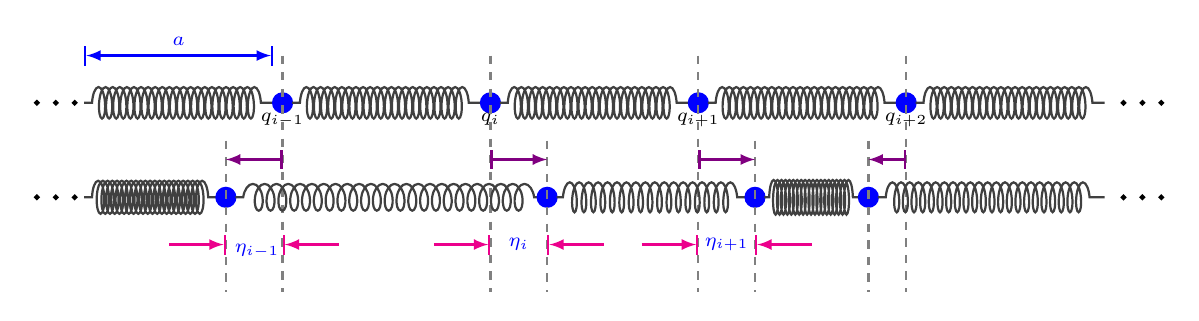
\begin{tikzpicture}[black!75,thick, scale=1.2]
\filldraw[black](-0.1,2)circle(0.5pt) node[below, black] {};
\filldraw[black](-0.3,2)circle(0.5pt) node[below, black] {};
\filldraw[black](-0.5,2)circle(0.5pt) node[below, black] {};
\draw[blue, |<->|, >=latex ](0,2.5) -- (2,2.5);
\node[above, blue] at (1,2.5){\scriptsize{$a$}};
\draw[decoration={coil, aspect=0.3, segment length=0.9mm, amplitude=2mm, pre length=1mm, post length=1mm}, decorate] (0,2) -- (2,2) node[midway,right=0.25cm,black]{}; 
\filldraw[blue](2.1,2)circle(1mm) node[below, black] {\scriptsize{$q_{i-1}$}};
\draw[dashed, gray](2.1,2.5)--(2.1,0);
\draw[decoration={coil, aspect=0.3, segment length=0.9mm, amplitude=2mm, pre length=1mm, post length=1mm}, decorate] (2.2,2) -- (4.2,2) node[midway,right=0.25cm,black]{}; 
\filldraw[blue](4.3,2)circle(1mm) node[below, black] {\scriptsize{$q_{i}$}};
\draw[dashed, gray](4.3,2.5)--(4.3,0);
\draw[decoration={coil, aspect=0.3, segment length=0.9mm, amplitude=2mm, pre length=1mm, post length=1mm}, decorate] (4.4,2) -- (6.4,2) node[midway,right=0.25cm,black]{}; 
\filldraw[blue](6.5,2)circle(1mm) node[below, black] {\scriptsize{$q_{i+1}$}};
\draw[dashed, gray](6.5,2.5)--(6.5,0);
\draw[decoration={coil, aspect=0.3, segment length=0.9mm, amplitude=2mm, pre length=1mm, post length=1mm}, decorate] (6.6,2) -- (8.6,2) node[midway,right=0.25cm,black]{}; 
\filldraw[blue](8.7,2)circle(1mm) node[below, black] {\scriptsize{$q_{i+2}$}};
\draw[dashed, gray](8.7,2.5)--(8.7,0);
\draw[decoration={coil, aspect=0.3, segment length=0.9mm, amplitude=2mm, pre length=1mm, post length=1mm}, decorate] (8.8,2) -- (10.8,2) node[midway,right=0.25cm,black]{}; 
\filldraw[black](11,2)circle(0.5pt) node[below, black] {};
\filldraw[black](11.2,2)circle(0.5pt) node[below, black] {};
\filldraw[black](11.4,2)circle(0.5pt) node[below, black] {};
%Resorte de Abajo
\filldraw[black](-0.1,1)circle(0.5pt) node[below, black] {};
\filldraw[black](-0.3,1)circle(0.5pt) node[below, black] {};
\filldraw[black](-0.5,1)circle(0.5pt) node[below, black] {};
\draw[decoration={coil, aspect=0.3, segment length=0.6mm, amplitude=2.1mm, pre length=1mm, post length=1mm}, decorate] (0,1) -- (1.4,1) node[midway,right=0.25cm,black]{}; 
\filldraw[blue](1.5,1)circle(1mm) node[below, black]{\scriptsize{}};
\draw[dashed, gray](1.5,1.6)--(1.5,0);
\draw[violet, <-|, >=latex ](1.5,1.4) -- (2.1,1.4);
\draw[magenta, ->|, >=latex ](0.9,0.5) -- (1.5,0.5);
\draw[magenta, |<-, >=latex ](2.1,0.5) -- (2.7,0.5);
\node[above, blue] at (1.83,0.25){\scriptsize{$\eta_{i-1}$}};
\draw[decoration={coil, aspect=0.5, segment length=1.5mm, amplitude=1.7mm, pre length=1mm, post length=0.8mm}, decorate] (1.6,1) -- (4.85,1) node[midway,right=0.25cm,black]{}; 
\filldraw[blue](4.9,1)circle(1mm) node[below, black] {\scriptsize{}};
\draw[dashed, gray](4.9,1.6)--(4.9,0);
\draw[violet, |->, >=latex ](4.3,1.4) -- (4.9,1.4);
\draw[magenta, ->|, >=latex ](3.7,0.5) -- (4.3,0.5);
\draw[magenta, |<-, >=latex ](4.9,0.5) -- (5.5,0.5);
\node[blue] at (4.6,0.5){\scriptsize{$\eta_{i}$}};
\draw[decoration={coil, aspect=0.3, segment length=1.2mm, amplitude=1.9mm, pre length=0.8mm, post length=0.5mm}, decorate] (5,1) -- (7,1) node[midway,right=0.25cm,black]{}; 
\filldraw[blue](7.1,1)circle(1mm) node[below, black]{\scriptsize{}};
\draw[dashed, gray](7.1,1.6)--(7.1,0);
\draw[violet, |->, >=latex ](6.5,1.4) -- (7.1,1.4);
\draw[magenta, ->|, >=latex ](5.9,0.5) -- (6.5,0.5);
\draw[magenta, |<-, >=latex ](7.1,0.5) -- (7.7,0.5);
\node[blue] at (6.8,0.5){\scriptsize{$\eta_{i+1}$}};
\draw[decoration={coil, aspect=0.2, segment length=0.5mm, amplitude=2.2mm, pre length=0.6mm, post length=0.5mm}, decorate] (7.2,1) -- (8.2,1) node[midway,right=0.25cm,black]{}; 
\filldraw[blue](8.3,1)circle(1mm) node[below, black]{\scriptsize{}};
\draw[dashed, gray](8.3,1.6)--(8.3,0);
\draw[violet, <-|, >=latex ](8.3,1.4) -- (8.7,1.4);
\draw[decoration={coil, aspect=0.3, segment length=1.1mm, amplitude=1.9mm, pre length=1mm, post length=1mm}, decorate] (8.4,1) -- (10.8,1) node[midway,right=0.25cm,black]{}; 
\filldraw[black](11,1)circle(0.5pt) node[below, black] {};
\filldraw[black](11.2,1)circle(0.5pt) node[below, black] {};
\filldraw[black](11.4,1)circle(0.5pt) node[below, black] {};
\end{tikzpicture} 
\caption{\emph{Sistema discreto de masas idénticas puntuales unidas por resortes con las mismas características.} \scriptsize{Fuente: Hecha en este proyecto}}
\label{osciladores}
\end{figure}

%--------------------------------------------------------------------------------------------------


\noindent
Utilizaremos como ejemplo ilustrativo, las vibraciones longitudinales de una varilla infinita. Se partir\'{a} entonces del sistema discreto que consiste en una cadena infinita de masas iguales espaciadas una distancia $a$, y conectadas a trav\'{e}s de resortes sin masa y uniformes (ver Fig.\ref{osciladores}), todos con la misma constante el\'{a}stica $k$.\\

\noindent
La infinitud de la cadena evita por el momento trabajar el problema de las condiciones de frontera (en los extremos). Se asumir\'{a} que las masas puntuales s\'{o}lo se pueden mover a lo largo de la cadena, en peque\~{n}as oscilaciones alrededor del punto de equilibrio. Denotando $\eta _{i}$ al desplazamiento de la $i$-esima part\'{\i}cula a partir de su posici\'{o}n de equilibrio, su energ\'{\i}a cin\'{e}tica es:

\begin{equation}
T=\frac{1}{2}\sum\limits_{i}m\dot{\eta}_{i}^{2}~,  \label{2.17a}
\end{equation}
\noindent
donde $m$ es la masa de cada part\'{\i}cula. La energ\'{\i}a potencial
correspondiente, resulta ser la suma de las energ\'{\i}as potenciales de
cada resorte, que surgen como resultado del estiramiento o compresi\'{o}n de
los mismos, as\'{\i}:

\begin{equation}
V=\frac{1}{2}\sum\limits_{i}k\left( \eta _{i+1}-\eta _{i}\right) ^{2}~.
\label{2.17b}
\end{equation}

\noindent
de manera que el lagrangiano que describe el sistemas es:

\begin{eqnarray}
L &=&T-V  \notag \\
&=&\sum\limits_{i}\left\{ \frac{1}{2}m\dot{\eta}_{i}^{2}-\frac{1}{2}k\left(
\eta _{i+1}-\eta _{i}\right) ^{2}\right\} ~,
\end{eqnarray}

\noindent
el cual puede ser escrito como:

\begin{eqnarray}
L &=&\frac{1}{2}\sum\limits_{i}a\left\{ \frac{m}{a}\dot{\eta}%
_{i}^{2}-ka\left( \frac{\eta _{i+1}-\eta _{i}}{a}\right) ^{2}\right\}  \notag
\\
&=&a\sum\limits_{i}L_{i}~,
\end{eqnarray}

\noindent
donde 
\begin{equation*}
L_{i}\equiv \frac{m}{a}\dot{\eta}_{i}^{2}-ka\left( \frac{\eta _{i+1}-\eta
_{i}}{a}\right) ^{2}~,
\end{equation*}

\noindent
y $a$ es la distancia entre los puntos del equilibrio.\\


Ahora se obtienen las ecuaciones de movimiento de Lagrange correspondientes
a las coordenadas $\eta _{i}$, de manera que se calcula:

\begin{eqnarray}
\frac{\partial L}{\partial \dot{\eta}_{k}} &=&\frac{1}{2}\sum\limits_{i}a%
\frac{\partial }{\partial \dot{\eta}_{k}}\left\{ \frac{m}{a}\dot{\eta}%
_{i}^{2}-ka\left( \frac{\eta _{i+1}-\eta _{i}}{a}\right) ^{2}\right\}  \notag
\\
&=&\sum\limits_{i}m\dot{\eta}_{i}\frac{\partial \dot{\eta}_{i}}{\partial 
\dot{\eta}_{k}}=\sum\limits_{i}m\dot{\eta}_{i}\delta _{ik}=m\dot{\eta}_{k}~,
\label{2.17d}
\end{eqnarray}

\begin{eqnarray}
\frac{\partial L}{\partial \eta _{k}} &=&\frac{1}{2}\sum\limits_{i}a\frac{%
\partial }{\partial \eta _{k}}\left\{ \frac{m}{a}\dot{\eta}_{i}^{2}-ka\left( 
\frac{\eta _{i+1}-\eta _{i}}{a}\right) ^{2}\right\} =-\frac{1}{2}%
\sum\limits_{i}\left\{ 2k\left( \eta _{i+1}-\eta _{i}\right) \frac{\partial
\left( \eta _{i+1}-\eta _{i}\right) }{\partial \eta _{k}}\right\}  \notag \\
&=&-\sum\limits_{i}k\left( \eta _{i+1}-\eta _{i}\right) \left[ \frac{%
\partial \eta _{i+1}}{\partial \eta _{k}}-\frac{\partial \eta _{i}}{\partial
\eta _{k}}\right] =-\sum\limits_{i}k\left( \eta _{i+1}-\eta _{i}\right) %
\left[ \delta _{i+1,k}-\delta _{ik}\right]  \notag \\
&=&-k\left[ \left( \eta _{k}-\eta _{k-1}\right) -\left( \eta _{k}-\eta
_{k+1}\right) \right] ~.  \label{2.17e}
\end{eqnarray}

\noindent
Entonces, al usar las ecuaciones de Lagrange para las coordenadas generalizadas $\eta _{k}$,
\begin{equation}
\frac{d}{dt}\left( \frac{\partial L}{\partial \dot{\eta}_{k}}\right) -\frac{%
\partial L}{\partial \eta _{k}}=0~,  \label{2.17c}
\end{equation}

\noindent
y empleando (\ref{2.17d}) con (\ref{2.17e}) se deriva

\begin{eqnarray}
m\ddot{\eta}_{i}-k\left[ \left( \eta _{i+1}-\eta _{i}\right) +\left(\eta_{i}-\eta _{i-1}\right) \right]=0~,  \label{2.17f}
\end{eqnarray}

\noindent 
donde se ha hecho el cambio de índice mudo $k \rightarrow i$. Dividiendo\ (\ref{2.17f}) entre $a$ implica:

\begin{equation}
\frac{m}{a}\ddot{\eta}_{i}-ka\frac{\left(\eta _{i+1}-\eta_{i}\right)}{a^{2}}+ka\frac{\left( \eta_{i}-\eta _{i-1}\right) }{a^{2}}=0~.
\label{2.17g}
\end{equation}
\noindent
Las anteriores ecuaciones se escogieron de esa forma con el fin de obtener una interpretaci\'{o}n sencilla de los par\'{a}metros en el l\'{\i}mite cuando $a\rightarrow 0$.\\
Es claro por ejemplo, que $m/a$ se reduce en el cont\'{\i}nuo a la densidad lineal de masa que se denota por $\mu$. No obstante, el l\'{\i}mite de $ka$ no es tan directo. Para una varilla el\'{a}stica que obedece la ley de Hooke, la elongaci\'{o}n de la varilla por unidad de longitud es proporcional a la fuerza o tensi\'{o}n ejercida a lo largo de \'{e}sta, lo cual se puede escribir como:

\begin{equation*}
F=Y\xi ~,
\end{equation*}

\noindent
donde $\xi $ es la enlongaci\'{o}n por unidad de longitud y $Y$ el modulo de Young. Por otro lado, la elongaci\'{o}n de un segmento $a$, por unidad de longitud del sistema discreto en cuesti\'{o}n, se escribe como:

\begin{equation*}
\xi =\frac{\eta _{i+1}-\eta _{i}}{a}~,
\end{equation*}
\noindent
la fuerza necesaria para estirar el resorte en esta cantidad es

\begin{equation}
F=k\left( \eta _{i+1}-\eta _{i}\right) =ka\left( \frac{\eta _{i+1}-\eta _{i}%
}{a}\right) ~,
\end{equation}

\noindent
indicando que $ka$ debe corresponder al m\'{o}dulo de Young $Y$ de la varilla cont\'{\i}nua. Al ir del sistema discreto al cont\'{\i}nuo, el \'{\i}ndice $i$, que identifica a una masa puntual espec\'{\i}fica, se convierte en una coordenada cont\'{\i}nua de posici\'{o}n $x$, de manera que en vez de la variable discreta $q_{i}$ ahora se tendr\'{\i}a una
variable de campo cont\'{\i}nua que para este problema es $\eta (x)$. Adicionalmente, la cantidad

\begin{equation}
\underset{a\rightarrow 0}{\lim }\frac{\eta _{i+1}-\eta _{i}}{a}=\underset{%
a\rightarrow 0}{\lim }\frac{\eta \left( x+a\right) -\eta \left( x\right) }{a}%
=\frac{d\eta }{dx}~,
\end{equation}
\noindent
se interpreta como una derivada de la variable de campo en relaci\'{o}n a una coordenada continua, de modo que $a$ hace el rol de $dx$.\\

\noindent
Finalmente, la suma sobre el \'{\i}ndice discreto $i$ se convierte en una integral sobre $x$ a lo largo de la longitud de la varilla. El Lagrangiano del sistema adquiere la forma

\begin{eqnarray}
L &=&\frac{1}{2}\sum\limits_{i}\left\{ a\frac{m}{a}\dot{\eta}_{i}^{2}-ka\left( \frac{\eta _{i+1}-\eta _{i}}{a}\right) ^{2}\right\}=\sum\limits_{i}aL_{i}~,~~~~~\text{(de lo discreto)}  \notag 
\end{eqnarray}
\noindent a
\begin{eqnarray}
L &=&\frac{1}{2}\int dx\ \left\{ \mu \dot{\eta}^{2}-Y\left( \frac{d\eta }{dx}\right) ^{2}\right\} \equiv \int dx  \mathcal{L}~.~~~~~\text{(En el continuo)}  \label{2.17h}
\end{eqnarray}

\vspace{0.3cm}
\noindent
Observe, que en el l\'{\i}mite cuando $a\rightarrow 0$, los \'{u}ltimos dos t\'{e}rminos de la ecuaci\'{o}n de movimiento (\ref{2.17g}) asociados a las coordenadas $\eta $ se convierten en:

\begin{eqnarray*}
ka\frac{\left(\eta _{i}-\eta _{i-1}\right) }{a^{2}}-ka\frac{\left(\eta_{i+1}-\eta_{i}\right) }{a^{2}}~\ &\implies &~\ \ Y\frac{\left( \eta_{i}-\eta_{i-1}\right) }{a^{2}}-Y\frac{\left( \eta _{i+1}-\eta_{i}\right) }{a^{2}}\qquad  \notag \\
\frac{Y}{a}\left[ \frac{\left( \eta_{i}-\eta _{i-1}\right) }{a}-\frac{\left( \eta_{i+1}-\eta_{i}\right) }{a}\right] ~\ &\implies &~\ \frac{Y}{a}\left[ \left( \frac{\eta \left( x\right) -\eta \left( x-a\right) }{a}\right)-\left( \frac{\eta \left( x+a\right) -\eta \left( x\right) }{a}\right)\right] ~,  \label{2.17i}
\end{eqnarray*}
\noindent
que en términos de derivadas se interpreta como siendo,
\begin{equation*}
\lim_{a\rightarrow 0}ka\left[ \left( \frac{\eta _{i}-\eta _{i-1}}{a^{2}}\right) -\left( \frac{\eta _{i+1}-\eta _{i}}{a^{2}}\right) \right] =\frac{Y}{a}\left[ \left( \frac{d\eta \left( x\right) }{dx}\right) _{x-a}-\left( \frac{d\eta}{dx}\right) _{x}\right]~.
\end{equation*}

\noindent
Al considerar nuevamente el l\'{\i}mite cuando $a\rightarrow 0$,

\begin{eqnarray}
\underset{a\rightarrow 0}{\lim }\frac{Y}{a}\left[ \left( \frac{d\eta (x)}{dx}\right) _{x-a}-\left( \frac{d\eta (x)}{dx}\right) _{x}\right] &=&-Y\underset{a\rightarrow 0}{\lim }\frac{1}{a}\left[ \left( \frac{d\eta (x)}{dx}\right)_{x}-\left( \frac{d\eta (x)}{dx}\right) _{x-a}\right]  \notag \\
&=&-Y\frac{d}{dx}\left( \frac{d\eta (x)}{dx}\right) \notag \\
&=&-Y\frac{d^{2}\eta (x)}{dx^{2}}~.  \label{2.17j}
\end{eqnarray}

\noindent
Por lo tanto, la extensi\'{o}n al cont\'{\i}nuo de la ecuaci\'{o}n de
movimiento (\ref{2.17g}) para la varilla el\'{a}stica es:

\begin{equation}
\frac{m}{a}\ddot{\eta}_{k}-ka\frac{\left( \eta _{k+1}-\eta _{k}\right) }{%
a^{2}}+ka\frac{\left( \eta _{k}-\eta _{k-1}\right) }{a^{2}}=0\ \implies ~\
\mu \frac{d^{2}\eta }{dt^{2}}-Y\frac{d^{2}\eta }{dx^{2}}=0~,
\label{2.17k}
\end{equation}

\noindent lo que se reescribe como
\begin{equation}
\frac{d^{2}\eta }{dt^{2}}=\frac{Y}{\mu }\frac{d^{2}\eta }{dx^{2}}~.
\label{Eonda}
\end{equation}

\noindent
La relaci\'{o}n (\ref{Eonda}) se conoce como ecuaci\'{o}n diferencial de onda unidimensional, para este caso longitudinal y que se propaga en un medio el\'{a}stico con velocidad:

\begin{equation*}
v=\sqrt{\frac{Y}{\mu}}~.
\end{equation*}

\vspace{1cm}
Este ejemplo sencillo ilustra la mayor parte de las caracter\'{\i}sticas generales que presenta el paso al cont\'{\i}nuo. Un aspecto muy relevante es el papel de la coordenada de posici\'{o}n $x$. Esta variable no representa una coordenada generalizada, es simplemente el \'{\i}ndice cont\'{\i}nuo que reemplaza al \'{\i}ndice $i$. As\'{\i}, como cada diferente valor de $i$ corresponde a una coordenada generalizada diferente $\eta _{i}$ del sistema discreto, de la misma forma hay una coordenada generalizada $\eta \left(x\right) $ por cada valor de $x$ en el sistema cont\'{\i}nuo. Dado que $\eta$ tambi\'{e}n es en general funci\'{o}n del par\'{a}metro cont\'{\i}nuo tiempo debemos escribir $\eta \left( x,t\right) $, esto indica que $x$ al igual que el tiempo se puede considerar como un par\'{a}metro que entra en el Lagrangiano y que estan rotulando al espacio y tiempo. Si el sistema cont\'{\i}nuo fuera tridimensional en lugar de unidimensional, las coordenadas generalizadas se rotular\'{\i}an con tres \'{\i}ndices cont\'{\i}nuos $x$, $y$, $z$ y las coordenadas generalizadas se escribir\'{\i}an como $\eta
(x,y,z,t)$.\\

\noindent
Vale la pena enfatizar que en la formulaci\'{o}n en el cont\'{\i}nuo, las cantidades $x$, $y$, $z$, $t$ son completamente independientes unas de otras, y solo aparecen como variables expl\'{\i}citas en $\eta$ en este caso. Por lo tanto, las derivadas de $\eta $ con respecto a cualquiera de ellas se pueden escribir como derivadas totales sin ninguna ambig\"{u}edad\footnote{Para evitar confusión con otros textos se las trabajara como derivadas parciales sabiendo que cada parámetro es independiente entre sí.}. Por otro lado la ecuaci\'{o}n asociada al lagrangiano (\ref{2.17h}) indica que este se escribe como una integral sobre el \'{\i}ndice cont\'{\i}nuo $x$, donde $\mathcal{L}$ caracteriza al integrando. Entonces en el correspondiente caso tridimensional el lagrangiano tendr\'{a} la forma:
\begin{equation}
L=\int d^{3}x\ \mathcal{L}~,  \label{2.17l}
\end{equation}

\noindent
siendo $\mathcal{L}$ la correspondiente \textbf{densidad lagrangiana}, que para una serie de vibraciones longitudinales en la varilla de acuerdo a (\ref{2.17h}), viene dada por:

\begin{equation}
\mathcal{L}=\frac{1}{2}\left[ \mu \dot{\eta}^{2}-Y\left( \frac{d\eta }{dx}\right) ^{2}\right] ~.  \label{2.17m}
\end{equation}

Antes de entrar en detalle con la teoría clásica de campos, se hará un breve repaso de la formulacón lagrangiana en una dimensión para sistemas continuos.

\vspace{1cm}
\subsection{Formulaci\'{o}n Lagrangiana en una dimensi\'{o}n para sistemas cont\'{\i}nuos}
\vspace{0.5cm}
De la ecuaci\'{o}n (\ref{2.17m}) se observa que la densidad lagrangiana asociada a la varilla el\'{a}stica depende de $\dot{\phi}\equiv \frac{\partial \phi }{\partial t}$ y $\frac{\partial \phi }{\partial x}$, donde se ha hecho el cambio de notación en el campo $\eta \rightarrow \phi$. Esto indica que $x$ y $t$ juegan un rol similar como par\'{a}metros de la densidad Lagrangiana.\\
Si hubiera fuerzas locales presentes adem\'{a}s de las interacciones entre vecinos, se puede tener una $\mathcal{L}$ que dependa de $\phi$ como tal, adem\'{a}s del gradiente espacial de $\phi$ y su derivada
temporal. En el caso m\'{a}s general la densidad lagrangiana puede ser tambi\'{e}n funci\'{o}n expl\'{\i}cita de $x$ y $t$ como es el caso de un campo externo que no sea constante ni uniforme. Entonces, la densidad Lagrangiana
para un sistema cont\'{\i}nuo unidimensional aparece como una funci\'{o}n de la variable de campo $\phi$ en la forma:

\begin{equation}
\mathcal{L}=\mathcal{L}\left(\phi ,\frac{\partial \phi }{\partial t},\frac{\partial \phi }{\partial x}x,t\right) ~,  \label{2.17n}
\end{equation}

\noindent
siendo el lagrangiano total $L$, la integral de la densidad $\mathcal{L}$ sobre todo el
rango de valores de $x$ que define al sistema.\\

\noindent
\begin{cabox}
Al extender el formalismo Lagrangiano a sistemas continuos, es claro que dicho sistema será identificado por los campos $\phi(x,t)$ los cuales toman un valor en cada punto del espacio y también por una densidad lagrangiana. Por lo tanto, los campos son ahora los grados de libertad que caracterizan al sistema físico y junto con sus derivadas deberán describir completamente la dinámica del sistema.\\

\noindent
Ahora, dado al interés de estudiar teorías relativistas, esta densidad lagrangiana deberá ser \emph{invariante bajo transformaciones de Lorentz}, es decir deberá ser un escalar, lo que va asegurar que las ecuaciones de campo sean coovariantes bajo estas transformaciones.\\
\end{cabox}

\noindent
Generalmente, para construir una densidad lagrangiana se considerarán polinomios en los campos y en sus derivadas aún cuando también existen modelos con términos no polinomiales los cuales se han y están estudiando. Otra característica de $\mathcal{L}$ es que sea una cantidad real, ya que hasta el momento ningún sistema clásico que se conozca sugiere una densidad compleja.\\

\noindent
La práctica ha demostrado que la densidad lagrangiana que describirá un sistema físico se puede escoger tan simple como sea posible, dado que una cantidad $\mathcal{L}$ , las expresiones $\mathcal{L}^{n}$ o alguna función de $\mathcal{L}$ son también invariantes por transformaciones de Lorentz. Así, se consideran las formas mas simples de funciones de los campos y sus derivadas los cuales serán suficientes para que su validez sea confirmada por los resultados experimentales, por esta razón se tendrá presente que la densidad Lagrangiana dependa en cada punto del espacio-tiempo, del valor del campo y sus derivadas evaluadas en dicho punto (o  en una vecindad del mismo). Cuando ocurre esto, se dice que la teoría es local.\\
Teorías donde el valor de un campo en un punto dependerá del valor del mismo campo evaluado en otro punto se llaman no locales; aún cuando estas teorías son concebibles, son demasiado complejas.\\


Para ser un poco más generales, e irnos familiarizarnos con la notación, la teoría que estamos considerando es de un solo campo $\phi=\phi(x,t)$ donde $(x,t)$ representa un punto en el espacio-tiempo unidimensional, entonces la densidad lagrangiana (\ref{2.17n}) se reescribirá como:

\begin{equation}
    \mathcal{L}=\mathcal{L}(\phi,\partial_{0}\phi,\partial_{1}\phi)~,
\end{equation}

\noindent
donde hemos introducido la notación de relatividad especial:
\begin{equation*}
    \partial_{0}\phi \equiv \frac{\partial \phi}{\partial t}~~~~~,~~~~~\partial_{1}\phi \equiv \frac{\partial \phi}{\partial x}~.
\end{equation*}


Con el fin de encontrar las ecuaciones de movimiento asociadas a dicho lagrangiano, se construye la acción asociada al sistema físico, la cual debe ser invariante por transformaciones de Lorentz, así:

\begin{equation}
    S[\phi]=\int_{t_{1}}^{t_{2}} \int_{x_{1}}^{x_{2}} dt dx \mathcal{L}(\phi,\partial_{0}\phi,\partial_{1}\phi)~,
\end{equation}

\noindent
la cual es una funcional de los campos. Cabe resaltar, que esta cantidad contendrá mas información sobre el sistema físico que la misma densidad Lagrangiana, dado que ella permitirá deducir las ecuaciones de campo. Su definición como una integral abarca la región del espacio tiempo donde el sistema físico esta definido, así $S$ hace una descripción global del sistema.\\

Ahora, se procederá a obtener las ecuaciones de campo generalizando el principio de Hamilton de la mecánica clásica según el cual la acción debe ser un mínimo para los estados actuales del sistema, es decir, $S$ deberá ser un mínimo para aquellas funciones $\phi$ que son soluciones de las ecuaciones de campo,

\begin{equation}
    \delta S[\phi]=\delta \int_{t_{1}}^{t_{2}} \int_{x_{1}}^{x_{2}} dt dx \mathcal{L}(\phi,\partial_{0}\phi,\partial_{1}\phi)=0~,  \label{2.17o}
\end{equation}


\noindent
indicando que las ecuaciones de movimiento deben obtenerse haciendo una variaci\'{o}n de la integral asociada a $\mathcal{L}$. El procedimiento es muy similar al caso discreto, la variaci\'{o}n se hace solo sobre $\phi$ y sus derivadas; los par\'{a}metros $x$, $t$ no se ven afectados por la variaci\'{o}n o trav\'{e}s de los l\'{\i}mites de integrac\'{o}n.\\

\noindent
Además, en analogía con la mecánica clásica la variaci\'{o}n de $\phi$ se tomará nula en los extremos temporales $t_{1}$ y $t_{2}$, y en los extremos espaciales $x_{1}$, $x_{2}$ de la integraci\'{o}n en $x$, en otras palabras se tiene condici\'{o}n de extremo fijo en los par\'{a}metros.\\

\noindent
De igual manera que en el principio variacional de Hamilton discreto se considera una familia de caminos variados introducidos muy convenientemente, en el espacio de las $\phi$ ocurre los mismo, donde $\phi$ se escoge a partir de una familia uniparam\'{e}trica de las posibles funciones,

\begin{equation*}
\phi \left( x,t,\alpha \right) =\phi \left( x,t,0\right) +\alpha \zeta \left( x,t\right)~,
\end{equation*}

\noindent
siendo $\alpha$ el parámetro que caracteriza cada camino y $\zeta \left(x,t\right)$ cualquier funci\'{o}n bien comportada que se anula en los puntos extremos de $x$ y $t$. La característica que se impone es que $\phi (x,t,0)$ denote la funci\'{o}n correcta que satisface el principio de Hamilton,\\

\noindent
Si $S$ se considera una funci\'{o}n de $\alpha$, de tal modo que tenga un extremo en $\phi (x,t,0)$ la derivada de $S$ con respecto a $\alpha $ se anula en $\alpha =0$ dado que esa es la trayectoria real que seguir\'{a} el sistema. Con base en esto y a trav\'{e}s de la diferenciaci\'{o}n directa se obtiene:

\begin{eqnarray}
\frac{dS}{d\alpha } &=&\frac{d}{d\alpha }\int_{t_{1}}^{t_{2}}\int_{x_{1}}^{x_{2}}dtdx\mathcal{L}=\int_{t_{1}}^{t_{2}}\int_{x_{1}}^{x_{2}}dtdx\frac{\partial \mathcal{L}}{\partial \alpha } \notag \\
&=&\int_{t_{1}}^{t_{2}}\int_{x_{1}}^{x_{2}}dtdx\left[ \frac{\partial \mathcal{L}}{\partial \phi }\frac{\partial \phi }{\partial \alpha }+\frac{\partial \mathcal{L}}{\partial \left( \partial _{0}\phi \right) }\frac{\partial \left( \partial _{0}\phi \right) }{\partial \alpha }+\frac{\partial \mathcal{L}}{\partial \left( \partial _{1}\phi \right) }\frac{\partial \left( \partial _{1}\phi \right) }{\partial \alpha }\right] ~,
\label{2.17p}
\end{eqnarray}

\noindent
sin embargo, puede ocurrir el hecho que $\mathcal{L}$ dependa expl\'{\i}citamente de $x$ y $t$, pero estos t\'{e}rminos no aparecen en la derivada anterior en virtud de que $\partial x/\partial \alpha =\partial t/\partial \alpha =0$, debido a que los par\'{a}metros no cambian cuando se hace una variaci\'{o}n del campo $\phi (x,t)$. Ahora bien, debido a que la variaci\'{o}n de $\phi$ representada por $\alpha \zeta \left( x,t\right) $, se anula en los extremos de ambos par\'{a}metros, una integraci\'{o}n por partes en $x$
y $t$ genera las relaciones:

\begin{equation}
\int_{t_{1}}^{t_{2}}dt\frac{\partial \mathcal{L}}{\partial \left( \partial_{0}\phi \right) }\frac{\partial \left( \partial _{0}\phi \right) }{\partial \alpha }=-\int_{t_{1}}^{t_{2}}dt\frac{d}{dt}\left[ \frac{\partial \mathcal{L}}{\partial \left( \partial _{0}\phi \right) }\right] \frac{\partial \phi }{\partial \alpha }~,
\label{2.17q}
\end{equation}

y

\begin{equation}
\int_{x_{1}}^{x_{2}}dx\frac{\partial \mathcal{L}}{\partial \left( \partial_{1}\phi \right) }\frac{\partial \left( \partial _{1}\phi \right) }{\partial \alpha }=-\int_{x_{1}}^{x_{2}}dx\frac{d}{dx}\left[ \frac{\partial \mathcal{L}}{\partial \left( \partial _{1}\phi \right) }\right] \frac{\partial \phi }{\partial \alpha }~.
\label{2.17r}
\end{equation}

Con estos resultados, la ecuación (\ref{2.17p}) se escribe,

\begin{equation*}
\frac{dS}{d\alpha }=\int_{t_{1}}^{t_{2}}\int_{x_{1}}^{x_{2}}dt\ dx\ \zeta \left( x,t\right) \left\{ \frac{\partial \mathcal{L}}{\partial \phi }-\frac{d}{dt}\left[ \frac{\partial \mathcal{L}}{\partial \left( \partial _{0}\phi \right) }\right] -\frac{d}{dx}\left[ \frac{\partial \mathcal{L}}{\partial \left( \partial _{1}\phi \right) }\right] \right\} =0~,
\end{equation*}

\noindent
y dado que $\zeta(x,t)$ es una función arbitraria entonces el término entre llaves debe anularse, por lo tanto

\begin{equation}
\boxed{
\frac{\partial \mathcal{L}}{\partial \phi }-\frac{d}{dt}\left[ \frac{\partial \mathcal{L}}{\partial \left( \partial _{0}\phi \right) }\right]-\frac{d}{dx}\left[ \frac{\partial \mathcal{L}}{\partial \left( \partial_{1}\phi \right) }\right] =0~,  \label{2.17s}
}
\end{equation}

\noindent
así se obtiene lo que se conoce como las ecuaciones de Euler Lagrange, determinadas a partir del principio de Hamilton\ (\ref{2.17o})\ llevado al limite cont\'{\i}nuo.\\


Un sistema de $n$ grados de libertad posee $n$ ecuaciones de Lagrange, sin embargo, \textexclamdown \emph{pareciera que para un sistema cont\'{\i}nuo solo se tuviera una ecuaci\'{o}n de Lagrange}!. Recuerde que en el caso discreto la ecuaci\'{o}n de movimiento para cada $\eta _{i}$ es una ecuaci\'{o}n diferencial que solo involucra al tiempo, en tal sentido la ultima ecuaci\'{o}n (\ref{2.17s}) nos da una ecuaci\'{o}n de movimiento para cada valor del \emph{\'{\i}ndice}\ cont\'{\i}nuo $x$. La naturaleza cont\'{\i}nua de $x$ se manifiesta en que la ecuaci\'{o}n (\ref{2.17s}) es una ecuaci\'{o}n diferencial parcial en $x$ y $t$, cuya soluci\'{o}n es de la forma $\phi \left( x,t\right) $. De lo anterior se desprende adem\'{a}s que la dimensi\'{o}n del espacio de configuraciones corresponde a la cardinalidad del espacio real (en una dos o tres dimensiones) ya que cada \'{\i}ndice cont\'{\i}nuo $x$ corresponde a un eje en el espacio de configuraciones.

\vspace{0.2cm}
\begin{exercise}
Usando integraci\'{o}n por partes, demostrar las relaciones (\ref{2.17q}) y (\ref{2.17r}).
\end{exercise}

\begin{solution}
Para mostrar (\ref{2.17q}) se utiliza la integral 

\begin{equation}
\int_{t_{1}}^{t_{2}}dt\ \frac{\partial \mathcal{L}}{\partial \left( \partial_{0}\phi \right) }\frac{\partial \left( \partial _{0}\phi \right) }{\partial \alpha }~,  \label{2.17ea}
\end{equation}

\noindent
al aplicar integraci\'{o}n por partes, se cumple $\int_{a}^{b}udv=\left. uv\right\vert _{a}^{b}-\int_{a}^{b}vdu$. Al definir 

\begin{equation*}
u\equiv \frac{\partial \mathcal{L}}{\partial \left( \partial _{0}\phi
\right) }~\ \ ~\ ,~\ \ \ \ dv=\frac{\partial \left( \partial _{0}\phi
\right) }{\partial \alpha }~dt\ ~\ \implies ~\ ~\ du\equiv \frac{d}{dt}%
\left( \frac{\partial \mathcal{L}}{\partial \left( \partial _{0}\phi \right) 
}\right) ~\ \ ~\ ,~\ \ \ \ v=\frac{\partial \phi }{\partial \alpha }~,
\label{2.17eb}
\end{equation*}

\noindent
y reemplazando en (\ref{2.17ea}), 
\begin{eqnarray*}
\int_{t_{1}}^{t_{2}}dt\ \frac{\partial \mathcal{L}}{\partial \left( \partial_{0}\phi \right) }\frac{\partial \left( \partial _{0}\phi \right)}{\partial \alpha } &=&\left. \frac{\partial \mathcal{L}}{\partial \left( \partial_{0}\phi \right) }\frac{\partial \phi }{\partial \alpha }\right\vert_{t_{1}}^{t_{2}}-\int_{t_{1}}^{t_{2}}dt\ \frac{d}{dt}\left[ \frac{\partial \mathcal{L}}{\partial \left( \partial _{0}\phi \right) }\right] \frac{\partial \phi }{\partial \alpha } \\
&=&\underset{0}{\underbrace{\left. \frac{\partial \mathcal{L}}{\partial \left( \partial _{0}\phi \right) }\zeta \left( x,t\right) \right\vert_{t_{1}}^{t_{2}}}}-\int_{t_{1}}^{t_{2}}dt\ \frac{d}{dt}\left[ \frac{\partial \mathcal{L}}{\partial \left( \partial _{0}\phi \right) }\right] \frac{\partial \phi }{\partial \alpha }~\ ,
\end{eqnarray*}
\begin{equation}
\therefore ~\ \ \int_{t_{1}}^{t_{2}}dt\ \frac{\partial \mathcal{L}}{\partial
\left( \partial _{0}\phi \right) }\frac{\partial \left( \partial _{0}\phi
\right) }{\partial \alpha }=-\int_{t_{1}}^{t_{2}}dt\ \frac{d}{dt}\left[ 
\frac{\partial \mathcal{L}}{\partial \left( \partial _{0}\phi \right) }%
\right] \frac{\partial \phi }{\partial \alpha }~.  \label{2.17ec}
\end{equation}

\noindent
Por otro lado, para demostrar la ecuaci\'{o}n (\ref{2.17r}), se debe aplicar integraci\'{o}n por partes a la expresi\'{o}n: 
\begin{equation*}
\int_{x_{1}}^{x_{2}}dx\ \frac{\partial \mathcal{L}}{\partial \left( \partial
_{1}\phi \right) }\frac{\partial \left( \partial _{1}\phi \right) }{\partial
\alpha }~,
\end{equation*}

\noindent
pero al compararla con (\ref{2.17ea}), se diferencian \'{u}nicamente en el
cambio del par\'{a}metro $t$ a $x$. Entonces, 
\begin{equation}
\int_{x_{1}}^{x_{2}}dx\ \frac{\partial \mathcal{L}}{\partial \left( \partial
_{1}\phi \right) }\frac{\partial \left( \partial _{1}\phi \right) }{\partial
\alpha }=-\int_{x_{1}}^{x_{2}}dx\ \frac{d}{dx}\left[ \frac{\partial \mathcal{%
L}}{\partial \left( \partial _{1}\phi \right) }\right] \frac{\partial \phi }{%
\partial \alpha }~.  \label{2.17ed}
\end{equation}
\end{solution}

\subsection{Formulaci\'{o}n Lagrangiana en tres dimensiones para sistemas cont\'{\i}nuos con un n\'{u}mero arbitrario de variables de campo}
\vspace{0.2cm}
\subsection*{\textcolor{orange}{Teoría clásica de campos}}
\vspace{0.3cm}
La formulaci\'{o}n Lagrangiana desarrollada aqu\'{\i} debe ser extendida a situaciones en dos y tres dimensiones, como es el caso por ejemplo de un s\'{o}lido  el\'{a}stico tridimensional. Adicionalmente, en lugar de un solo campo $\phi$ se podr\'{\i}a tener varias de estas cantidades. A manera de ejemplo, en tres dimensiones un desplazamiento arbitrario con respecto a la posici\'{o}n de equilibrio se describir\'{\i}a por un vector espacial de campo $\vb{\phi}$ con tres componentes, en la formulaci\'{o}n de Lagrange esto implica tres campos ya que las coordenadas generalizadas deben ser escalares.\\

\noindent
La extensi\'{o}n a m\'{a}s dimensiones o m\'{a}s campos no presenta dificultades significativas. Sin embargo, la notaci\'{o}n se vuelve altamente engorrosa cuando pasamos por ejemplo a tres dimensiones. Se puede notar sin embargo que el principio de Hamilton (\ref{2.17o}) y las ecuaciones de Euler Lagrange (\ref{2.17s}) anteriormente preescritas presentan una alta simetr\'{\i}a con respecto a las variables de espacio y
tiempo, las variables espaciales junto con el tiempo parecen cumplir el mismo rol, siendo los campos funciones tanto de las coordenadas espaciales como del tiempo, donde todas ellas deben ser tratadas como variables independientes. No hay por ejemplo, variaci\'{o}n de los campos en los l\'{\i}mites de integraci\'{o}n en el principio de Hamilton tanto sobre el espacio como sobre el tiempo. Debe tenerse en cuenta sin embargo, que aunque en esta formulaci\'{o}n las coordenadas espaciales y temporales entran en forma m\'{a}s sim\'{e}trica,
el tiempo NO corresponde a un \'{\i}ndice para la coordenada generalizada $\phi (\mathbf{x},t)$, esto se puede ver del hecho de que en el sistema discreto el campo $\eta _{i}(t)$ est\'{a} rotulado por el \'{\i}ndice $i$ pero no por la variable temporal, la cual simplemente mide la evoluci\'{o}n de una coordenada generalizada espec\'{\i}fica $\eta _{i}$.\\

\noindent
En consecuencia de lo anterior, es conveniente trabajar con una notaci\'{o}n en t\'{e}rminos de un espacio de cuatro dimensiones con coordenadas $x^{0}=t $, $x^{1}=x$, $x^{2}=y$, $x^{3}=z$ (En unidades naturales). Esta notaci\'{o}n no tiene ning\'{u}n significado f\'{\i}sico adicional\footnote{Al no trabajar en unidades naturales, el factor $c$ en $x^{0}$ es la velocidad de la luz en el vac\'{\i}o y es usada s\'{o}lo con el fin de que $x^{0}$ tenga las mismas unidades que $x^{i}$.}. El tensor m\'{e}trico $g$ es el correspondiente a una geometr\'{\i}a euclidiana, donde las transformaciones del grupo de Galileo son las transformaciones de coordenadas permitidas sobre las componentes del espacio con el tensor m\'{e}trico restringido por $g_{ij}=\delta_{ij}$. Nuevamente se retomar\'{a} la convenci\'{o}n de suma sobre \'{\i}ndices repetidos, donde las variables de campo se rotular\'{a}n con el sub\'{\i}ndice $r$, donde $r$ contará el número de campos necesarios para estudiar el problema\footnote{En algunas ocasiones simbolizar\'{a} un \'{\i}ndice simple de dos, tres, cuatro o m\'{a}s valores, pero tambi\'{e}n puede simbolizar un conjunto de m\'{u}ltiples \'{\i}ndices. Por ejemplo, si la variable de campo es un tensor espacial de segundo rango, entonces $r$ realmente se refiere a dos sub\'{\i}ndices.}.\\

\noindent
Finalmente, una derivada de las variables de campo con respecto a cualquiera de las cuatro coordenadas $x^{\mu}$ se denotar\'{a} como:

\begin{equation*}
\partial _{\nu }\phi _{r}=\phi_{r,\nu }=\frac{\partial \phi _{r}}{\partial x^{\nu }}~\ ~\ \ ,\qquad \partial _{j}\phi =\phi _{,j}=\frac{\partial \phi }{\partial x^{j}}~\ \ \ ~,\qquad \partial _{\mu}\partial_{\nu }\phi _{i}=\phi_{i,\mu \nu }=\frac{\partial ^{2}\phi_{i}}{\partial x^{\mu }\partial x^{\nu }}~.
\end{equation*}

\noindent
S\'{o}lo las derivadas de las variables de campos ser\'{a}n simbolizadas de
esta manera. En esta notaci\'{o}n la densidad Lagrangiana asociada al sistema se expresará en la siguiente forma,

\begin{equation}
\mathcal{L}=\mathcal{L}\left( \phi_{r}(x),\partial_{\mu}\phi_{r}(x),x\right)~.  \label{2.17t}
\end{equation}
donde $x\equiv (x^{\nu})$ identificará un punto en el espacio-tiempo, $\phi_{r}=\left\{\phi_{1}(x),\phi_{2}(x),\ldots \right\}$ el conjunto de campos que describen el problema y $\partial_{\mu}\phi_{r} \equiv \left\{\partial_{\mu}\phi_{1}(x),\partial_{\mu}\phi_{2}(x),\ldots \right\}$.\\

\noindent
El Lagrangiano total en analogía con una dimensión, se interpreta como una integral sobre el espacio tridimensional de la forma

\begin{eqnarray}
L &=&\int d^{3}x\ \mathcal{L}\left( \phi_{r},\partial _{\mu }\phi_{r},x\right)~, \qquad ~~~d^{3}x\equiv dx^{1}dx^{2}dx^{3}~,  \label{2.17u}
\end{eqnarray}

\noindent
de tal manera que la acción asociada al sistema físico sea una funcional de los campos definida como,
\begin{equation}
    S[\phi]=\int d^{4}x \mathcal{L}\left( \phi _{r},\partial _{\mu }\phi_{r},x\right)~, \qquad ~~~d^{4}x\equiv dx^{0}dx^{1}dx^{2}dx^{3}~,
\end{equation}

\noindent
siendo su definición como una integral que abarca aquellas regiones del espacio-tiempo donde el sistema físico está definido.\\

\noindent
Para determinar las ecuaciones de campo, como se mostró anteriormente se generaliza el principio del Hamilton de la mecánica clásica, es decir $S$ deberá ser un mínimo para aquellas funciones $\phi(x)$ que son soluciones de
\begin{equation}
    \delta S[\phi(x)]=0~,
\end{equation}

\noindent
lo que se conoce como el principio de mínima acción el cual escrito como una integral en el espacio-tiempo es de la forma:

\begin{eqnarray}
\delta S[\phi] &=&\delta \int d^{4}x\ \mathcal{L}\left( \phi _{r},\partial _{\mu
}\phi_{r},x\right)=0~.  \label{2.18}
\end{eqnarray}

\noindent
Al construir la variación de la acción, los extremos que en este caso serán las fronteras se deben mantener fijos, es decir los campos deben permanecer constantes en el infinito, por lo tanto:

\begin{itemize}
    \item La variación de los campos en los extremos $t_{1}$ y $t_{2}$ debe ser nula.
    \begin{equation*}
        \delta\phi(\mathbf{x},t_{1})=\delta\phi(\mathbf{x},t_{2})=0~.
    \end{equation*}
    \item Los campos deberán tener un comportamiento asintótico en el infinito\footnote{Se puede interpretar como que la variaci\'{o}n de $\phi_{r}$ sea nula al evaluarla sobre la hipersuperficie  $\Sigma$ que delimita a la regi\'{o}n de integraci\'{o}n en el espacio y el tiempo.}, es decir que cuando $\left\vert \mathbf{x}\right\vert \rightarrow \infty $, se debe cumplir que $\phi(x,t)\rightarrow0$. 
\end{itemize}
\vspace{0.4cm}
\noindent
Aplicando estas consideraciones a la variación en la acción
\begin{equation}
\delta S\left[ \phi \right] =\int d^{4}x\left[ \frac{\partial \mathcal{L}}{\partial \phi _{r}}\delta \phi _{r}+\frac{\partial \mathcal{L}}{\partial \left( \partial _{\mu }\phi _{r}\right) }\delta \left( \partial _{\mu }\phi_{r}\right) \right] ~,
\label{2aa}
\end{equation}
el segundo término se reduce a:
\begin{equation*}
\int d^{4}x\frac{\partial \mathcal{L}}{\partial \left( \partial _{\mu }\phi_{r}\right) }\delta \left( \partial _{\mu }\phi _{r}\right) =\int d^{4}x~\partial _{\mu }\left[ \frac{\partial \mathcal{L}}{\partial \left( \partial _{\mu }\phi _{r}\right) }\delta \phi _{r}\right] -\int d^{4}x~\partial _{\mu }\left[ \frac{\partial \mathcal{L}}{\partial \left( \partial _{\mu }\phi _{r}\right) }\right] \delta \phi _{r}~,
\end{equation*}
\noindent
donde el primer término de la linea anterior se anula, dado que al extender el \emph{teorema de Stokes} a un espacio de 4 dimensiones se tiene:
\begin{equation}
\int_{V}d^{4}x~\partial _{\mu }\left[ \frac{\partial \mathcal{L}}{\partial
\left( \partial _{\mu }\phi _{r}\right) }\delta \phi _{r}\right]
=\oint_{\Sigma }da~n_{\mu }\left[ \frac{\partial \mathcal{L}}{\partial \left(
\partial _{\mu }\phi _{r}\right) }\delta \phi _{r}\right]~, 
\end{equation}
siendo $n^{\mu}$ el vector normal a la superficie. Por lo tanto la condición de contorno exige que
\begin{equation*}
\left. \frac{{}}{{}}\delta \phi_{r} \right\vert _{\Sigma }=0~.
\end{equation*}

\noindent
Así que la expresión (\ref{2aa}) se reduce a 
\begin{eqnarray}
\delta S\left[ \phi \right]  &=&\int d^{4}x\left[ \frac{\partial \mathcal{L}%
}{\partial \phi _{r}}\delta \phi _{r}-\partial _{\mu }\left( \frac{\partial 
\mathcal{L}}{\partial \left( \partial _{\mu }\phi _{r}\right) }\right)
\delta \phi _{r}\right] \notag \\
&=&\int d^{4}x\left[ \frac{\partial \mathcal{L}}{\partial \phi _{r}}%
-\partial _{\mu }\left( \frac{\partial \mathcal{L}}{\partial \left( \partial
_{\mu }\phi _{r}\right) }\right) \right] \delta \phi _{r}=0~. \label{2ab}
\end{eqnarray}
\noindent
El hecho que la variación que se realiza en los campos $\delta \phi_{r}$ es completamente arbitraria, la condición que deberá ser garantizada para poder satisfacer la identidad (\ref{2ab}), según el lema fundamental del cálculo de variaciones, es que:
\begin{equation}
\boxed{
\frac{\partial \mathcal{L}}{\partial \phi _{r}}-\partial _{\mu }\left( \frac{%
\partial \mathcal{L}}{\partial \left( \partial _{\mu }\phi _{r}\right) }%
\right), \quad\quad r=1,2,3,\ldots 
\label{elagrange}
}
\end{equation}
estas expresiones son conocidas como las ecuaciones de Euler-Lagrange y corresponden a las ecuaciones de campo descrito por $\phi_{r}\equiv \left\{\phi_{1}(x),\phi_{2}(x),\ldots\right\}$, de tal modo que estas soluciones tornarán estacionaria a la acción.

%En el apéndice \ref{Apendice B} se tiene otra manera de deducir las ecuaciones de Euler-Lagrange para sistemas continuos, la cuál se realiza con analogía en la mecánica clásica.\\

\noindent
Es sencillo ver que las ecuaciones (\ref{elagrange}) se reducen a el caso unidimensional (es decir con un s\'{o}lo par\'{a}metro espacial $x$), con una sola variable de campo (i.e. $r=1$). Comparando las dos ecuaciones se puede apreciar la ventaja de la notaci\'{o}n introducida (y a\'{u}n m\'{a}s si se introducen las tres dimensiones).\\

\noindent
En sistemas discretos, el Lagrangiano tiene un grado de arbitrariedad ya que se puede adicionar una derivada total en el tiempo de una funci\'{o}n arbitraria de las coordenadas generalizadas y el tiempo sin alterar las ecuaciones de movimiento. Con sistemas cont\'{\i}nuos, la densidad Lagrangiana posee una simetr\'{\i}a gauge similar bajo la adici\'{o}n de un t\'{e}rmino de la forma:

\begin{equation}
\mathcal{L}^{\prime }=\mathcal{L}+\partial _{\mu }F_{\mu}(\phi_{r},x)~,  \label{2.23}
\end{equation}

%recordando de nuevo que la derivada total en $x$ es equivalente a una
%derivada parcial, se puede escribir el segundo t\'{e}rmino en la forma:

%\begin{equation*}
%\frac{dF_{\mu} \left(\phi_{r},x\right)}{dx^{\mu }}=\frac{\partial F_{\mu}\left(\phi_{r},x\right)}{\partial x^{\mu }}=\partial _{\mu }F_{\mu}~.
%\end{equation*}

\noindent
siendo el último t\'{e}rmino la extensi\'{o}n del operador divergencia en 4 dimensiones. $F_{\mu}$ son cuatro funciones arbitrarias de las variables de campo $\phi_{r}$ y las coordenadas $x$. La aplicaci\'{o}n del teorema de la divergencia en el espacio de 4 dimensiones convierte la integral de hipervolumen en una integral sobre la hipersuperficie $\Sigma^{\mu }$ donde la variaci\'{o}n de $F_{\mu }$ es nula.

\begin{equation}
\delta \int d^{4}x\left[ \frac{{}}{{}}\partial _{\mu }F_{\mu }\left( \phi
_{r},x\right) \right] =\delta \oint_{\Sigma }ds^{\mu }F_{\mu }\left( \phi
_{r},x\right) =0~.
\end{equation}

\noindent
Esto significa que el segundo t\'{e}rmino a la derecha en (\ref{2.23}) no contribuye a la variaci\'{o}n de la acci\'{o}n y por tanto, tampoco contribuye a las ecuaciones de movimiento. Además, indica que la expresi\'{o}n (\ref{2.23}) es una transformaci\'{o}n gauge para la densidad Lagrangiana y representa una extensi\'{o}n natural del gauge visto en mec\'{a}nica anal\'{\i}tica para el caso discreto, con las asignaciones $q_{i}(t)\rightarrow \phi _{r}\left( x^{\mu }\right) $ , $\ L\rightarrow \mathcal{L}$, $F\rightarrow F_{\mu }$, $\ t\rightarrow x$. La \'{u}ltima asignaci\'{o}n tiene que ver con el hecho de que el problema discreto es uniparam\'{e}trico (s\'{o}lo el tiempo es un par\'{a}metro) y el problema en el cont\'{\i}nuo es multiparam\'{e}trico (con par\'{a}metros $t$, $x^{i}$).

\bigskip

\begin{exercise}
Estudiar el segundo término de la ecuación (\ref{2aa}).
\end{exercise}

\begin{solution}
La ecuaci\'{o}n (\ref{2aa}) representa una variaci\'{o}n en la acci\'{o}n,

\begin{equation*}
\delta S\left[ \phi \right] =\int d^{4}x\left[ \frac{\partial \mathcal{L}}{%
\partial \phi _{r}}\delta \phi _{r}+\frac{\partial \mathcal{L}}{\partial
\left( \partial _{\mu }\phi _{r}\right) }\delta \left( \partial _{\mu }\phi
_{r}\right) \right] ~,
\end{equation*}

analizando el segundo t\'{e}rmino de la relaci\'{o}n anterior:

\begin{eqnarray*}
\int d^{4}x\frac{\partial \mathcal{L}}{\partial \left( \partial _{\mu }\phi_{r}\right) }\delta \left( \partial _{\mu }\phi _{r}\right)  &=&\int d^{4}x\left[ \frac{\partial \mathcal{L}}{\partial \left( \partial _{0}\phi_{r}\right) }\delta \left( \partial _{0}\phi _{r}\right) +\frac{\partial \mathcal{L}}{\partial \left( \partial _{i}\phi _{r}\right) }\delta \left(\partial _{i}\phi _{r}\right) \right]  \\
&=&\int d^{4}x\left[ \frac{\partial \mathcal{L}}{\partial \left( \partial_{0}\phi _{r}\right) }\delta \left( \frac{\partial \phi _{r}}{\partial t} \right) +\frac{\partial \mathcal{L}}{\partial \left( \partial _{i}\phi_{r}\right) }\delta \left( \frac{\partial \phi _{r}}{\partial x^{i}}\right) \right] ,
\end{eqnarray*}

aqu\'{\i} se utiliza el hecho que la variaci\'{o}n $\delta \phi _{r}$ conmuta con las derivadas espaciales y temporales por el hecho de que esta cambia la forma del campo y no el punto espacio-temporal donde esta esta siendo evaluada, se tiene que

\begin{eqnarray}
\int d^{4}x\frac{\partial \mathcal{L}}{\partial \left( \partial _{\mu }\phi
_{r}\right) }\delta \left( \partial _{\mu }\phi _{r}\right)  &=&\int d^{4}x%
\left[ \frac{\partial \mathcal{L}}{\partial \left( \partial _{0}\phi
_{r}\right) }\partial _{0}\delta \phi _{r}+\frac{\partial \mathcal{L}}{%
\partial \left( \partial _{i}\phi _{r}\right) }\partial _{i}\delta \phi _{r}%
\right]   \notag \\
&=&\int d^{4}x\frac{\partial \mathcal{L}}{\partial \left( \partial _{\mu
}\phi _{r}\right) }\partial _{\mu }\delta \phi _{r},
\end{eqnarray}

empleando la propiedad de la derivada de un producto (o su equivalente integraci\'{o}n por partes),

\begin{eqnarray}
\partial _{\mu }\left[ \frac{\partial \mathcal{L}}{\partial \left( \partial
_{\mu }\phi _{r}\right) }\delta \phi _{r}\right]  &=&\partial _{\mu }\left( 
\frac{\partial \mathcal{L}}{\partial \left( \partial _{\mu }\phi _{r}\right) 
}\right) \delta \phi _{r}+\frac{\partial \mathcal{L}}{\partial \left(
\partial _{\mu }\phi _{r}\right) }\partial _{\mu }\delta \phi _{r}  \notag \\
\frac{\partial \mathcal{L}}{\partial \left( \partial _{\mu }\phi _{r}\right) 
}\partial _{\mu }\delta \phi _{r} &=&\partial _{\mu }\left[ \frac{\partial 
\mathcal{L}}{\partial \left( \partial _{\mu }\phi _{r}\right) }\delta \phi
_{r}\right] -\partial _{\mu }\left( \frac{\partial \mathcal{L}}{\partial
\left( \partial _{\mu }\phi _{r}\right) }\right) \delta \phi _{r}~,
\end{eqnarray}%
se tiene que%
\begin{eqnarray*}
\int d^{4}x\frac{\partial \mathcal{L}}{\partial \left( \partial _{\mu }\phi
_{r}\right) }\delta \left( \partial _{\mu }\phi _{r}\right)  &=&\int d^{4}x%
\left[ \partial _{\mu }\left( \frac{\partial \mathcal{L}}{\partial \left(
\partial _{\mu }\phi _{r}\right) }\delta \phi _{r}\right) -\partial _{\mu
}\left( \frac{\partial \mathcal{L}}{\partial \left( \partial _{\mu }\phi
_{r}\right) }\right) \delta \phi _{r}\right]  \\
&=&\int d^{4}x\partial _{\mu }\left( \frac{\partial \mathcal{L}}{\partial
\left( \partial _{\mu }\phi _{r}\right) }\delta \phi _{r}\right) -\int
d^{4}x\partial _{\mu }\left( \frac{\partial \mathcal{L}}{\partial \left(
\partial _{\mu }\phi _{r}\right) }\right) \delta \phi _{r}~,
\end{eqnarray*}%
al estudiar la integral%
\begin{eqnarray*}
\int d^{4}x\partial _{\mu }\left( \frac{\partial \mathcal{L}}{\partial
\left( \partial _{\mu }\phi _{r}\right) }\delta \phi _{r}\right)  &=&\int
d^{4}x\left[ \partial _{0}\left( \frac{\partial \mathcal{L}}{\partial \left(
\partial _{0}\phi _{r}\right) }\delta \phi _{r}\right) +\partial _{i}\left( 
\frac{\partial \mathcal{L}}{\partial \left( \partial _{i}\phi _{r}\right) }%
\delta \phi _{r}\right) \right]  \\
&=&\int d^{4}x\partial _{0}\left( \frac{\partial \mathcal{L}}{\partial
\left( \partial _{0}\phi _{r}\right) }\delta \phi _{r}\right) +\int
d^{4}x\partial _{i}\left( \frac{\partial \mathcal{L}}{\partial \left(
\partial _{i}\phi _{r}\right) }\delta \phi _{r}\right)  \\
&=&\int_{V}d^{3}x\int_{t_{1}}^{t_{2}}dt~\partial _{0}\left( \frac{\partial 
\mathcal{L}}{\partial \left( \partial _{0}\phi _{r}\right) }\delta \phi
_{r}\right)\\
&+&\int_{t_{1}}^{t_{2}}dt\int_{V}d^{3}x~\partial _{i}\left( \frac{\partial \mathcal{L}}{\partial \left( \partial _{i}\phi _{r}\right) }\delta \phi _{r}\right) ~,
\end{eqnarray*}
efectuando cada integral, donde se aplica el teorema de Stokes al segundo t%
\'{e}rmino se deduce que,%
\begin{equation*}
\int d^{4}x\partial _{\mu }\left( \frac{\partial \mathcal{L}}{\partial
\left( \partial _{\mu }\phi _{r}\right) }\delta \phi _{r}\right)
=\int_{V}d^{3}x\left. \left( \frac{\partial \mathcal{L}}{\partial \left(
\partial _{0}\phi _{r}\right) }\delta \phi _{r}\right) \right\vert
_{t_{1}}^{t_{2}}+\int_{t_{1}}^{t_{2}}dt\oint_{S}dS_{i}\left( \frac{\partial 
\mathcal{L}}{\partial \left( \partial _{i}\phi _{r}\right) }\delta \phi
_{r}\right) ~,
\end{equation*}%
este resultado permite establecer que: la primera integral se anula por la
condici\'{o}n de frontera $\delta \phi _{r}\left( \mathbf{x},t_{1}\right)
=\delta \phi _{r}\left( \mathbf{x},t_{2}\right) =0$. De igual manera, en la
segunda integral el integrando esta siendo evaluado en la superficie que
encierra el volumen en el cual est\'{a}n siendo considerados los campos. Si
este volumen se extiende en todo el espacio, la superficie que lo limita
tiende a infinito y del comportamiento asint\'{o}tico de los campos hace que
esta integral de superficie tienda a cero. De esta manera, deducimos que 
\begin{equation*}
\int d^{4}x\partial _{\mu }\left( \frac{\partial \mathcal{L}}{\partial
\left( \partial _{\mu }\phi _{r}\right) }\delta \phi _{r}\right) =0~,
\end{equation*}%
por lo tanto,%
\begin{equation*}
\int d^{4}x\frac{\partial \mathcal{L}}{\partial \left( \partial _{\mu }\phi
_{r}\right) }\delta \left( \partial _{\mu }\phi _{r}\right) =\int d^{4}x%
\frac{\partial \mathcal{L}}{\partial \left( \partial _{\mu }\phi _{r}\right) 
}\partial _{\mu }\delta \phi _{r}=-\int d^{4}x\partial _{\mu }\left( \frac{%
\partial \mathcal{L}}{\partial \left( \partial _{\mu }\phi _{r}\right) }%
\right) \delta \phi _{r}~,
\end{equation*}%
determinando que la variaci\'{o}n de la acci\'{o}n se reescriba como
\begin{equation}
\delta S\left[ \phi \right] =\int d^{4}x\left[ \frac{\partial \mathcal{L}}{%
\partial \phi _{r}}\delta \phi _{r}-\partial _{\mu }\left( \frac{\partial 
\mathcal{L}}{\partial \left( \partial _{\mu }\phi _{r}\right) }\right)
\delta \phi _{r}\right] ~.
\end{equation}
\end{solution}

\section{Formalismo Hamiltoniano en teoría Clásica de Campos}
\vspace{0.2cm}

El formalismo Hamiltoniano se puede extender a teoría de campos mientras se mantenga una completa analogía con la mecánica clásica.\\

La superioridad de la formulación Hamiltoniana en relación a la Lagrangiana, radica en el hecho que la primera reposa en el hecho de que la teoría deberá ser invariante por transformaciones canónicas las cuales son mucho mas generales que las transformación de coordenadas en la que se basa la formulación Lagrangiana. Así, desde el punto de vista Hamiltoniana la equivalencia de dos sistemas físicos implica la existencia de una transformación canónica tomando coordenadas y momentos de un sistema en las coordenadas y momentos del otro.\\

Al trabajar en teoría de campos, se define el momento canónico conjugado del campo $\phi_{r}$ como siendo,

\begin{equation}
    \pi_r (x) \equiv \fdv{\lagdn}{\dot{\phi}_r} = \pdv{\lagdn}{\dot{\phi}_r}~.
\end{equation}

El sistema físico ahora se definirá en el espacio de fase $(\phi_{r},\pi_{r})$. El Hamiltoniano canónico en este espacio es definido por

\begin{equation}
    H = \int \dd[3]{x} \pi_{r}(x)\dot{\phi}_r (x)-L = \int \dd[3]{x} \qty\Big[\pi_{r}(x)\dot{\phi}_r (x)-\lagdn] \equiv \int \dd[3]{x} \mathcal{H}.
    \label{HC}
\end{equation}

Aquí aparece la \emph{densidad hamiltoniana canónica} que se escribe como

\begin{equation} \boxed{
    \mathcal{H} = \pi_{r} \dot{\phi}_r-\lagdn \qty(\phi,\partial_{\mu}\phi) =\pdv{\lagdn}{\dot{\phi}_r} \dot{\phi}_r-\lagdn \qty(\phi,\partial_{\mu}\phi) .}
    \label{dHC}
\end{equation}

Los paréntesis de Poisson (PP) asociados a dos variables dinámicas $F(x) \equiv F[\phi,\pi]$ y $G(x) \equiv G[\phi,\pi]$ (representan dos funcionales) a tiempos iguales se calcula como

\begin{equation}
    \{F(x), G(y)\} \equiv \{F(x), G(y)\}_{x^0=x^0} \equiv \int \dd[3]{z} \left[\frac{\delta F(x)}{\delta \phi_r(z)} \frac{\delta G(y)}{\delta \pi_r(z)}-\frac{\delta G(y)}{\delta \phi_r(z)} \frac{\delta F(x)}{\delta \pi_r(z)}\right]
\end{equation}

A partir de esta expresión, es posible observar que los PP fundamentales entre las variables fundamentales del espacio de fase $\left(\phi_r, \pi_r\right)$, que se consideran linealmente independientes, son:

\begin{IEEEeqnarray}{rCl}
    \left\{\phi_r(x), \pi_s(y)\right\} &=& \int \dd[3]{z} \qty\Bigg[\frac{\delta \phi_r(x)}{\delta \phi_k(z)} \frac{\delta \pi_s(y)}{\delta \pi_k(z)}-\cancelto{0}{\frac{\delta \pi_s(y)}{\delta \phi_k(z)}}\cancelto{0}{\frac{\delta \phi_r(x)}{\delta \pi_k(z)}}] \notag \\
    &=& \int \dd[3]{z} \delta_{r k} \delta^3(x-z) \delta_{s k} \delta^3(y-z) \notag \\
    &=& \delta_{rs} \delta^3(x-y).
\end{IEEEeqnarray}

De igual manera se determina que

\begin{IEEEeqnarray*}{rCl}
    \left\{\phi_r(x), \phi_s(y)\right\} &=& \int \dd[3]{z} \qty\Bigg[ \frac{\delta \phi_r(x)}{\delta \phi_k(z)} \cancelto{0}{\frac{\delta \phi_s(y)}{\delta \pi_k(z)}} - \frac{\delta \phi_s(y)}{\delta \phi_k(z)} \cancelto{0}{\frac{\delta \phi_r(x)}{\delta \pi_k(z)}}]=0. \\
    \left\{\pi_r(x), \pi_s(y)\right\} &=& \int \dd[3]{z} \qty\Bigg[ \cancelto{0}{\frac{\delta \pi_r(x)}{\delta \phi_k(z)}} \frac{\delta \pi_s(y)}{\delta \pi_k(z)}-\cancelto{0}{\frac{\delta \pi_s(y)}{\delta \phi_k(z)}}_0 \frac{\delta \pi_r(x)}{\delta \pi_k(z)}]=0.
\end{IEEEeqnarray*}

En analogía con la mecánica clásica, la evolución temporal de una observable $F(x) \equiv F[\phi, \pi]$ es dada por:

\begin{equation}
    \dot{F}(x)=\left\{F(x), H \right\}.
\end{equation}

A partir de esta expresión, es posible determinar las correspondientes ecuaciones de Hamilton son,

\begin{IEEEeqnarray}{rCl}
    \dot{\phi}_r(x)=\left\{\phi_r(x), H\right\}=\int \dd[3]{z} \frac{\delta \phi_r(x)}{\delta \phi_k(z)} \frac{\delta H}{\delta \pi_k(z)}=\frac{\delta H}{\delta \pi_r(x)} \\
    \dot{\pi}_r(x)=\left\{\pi_i(x), H \right\}=-\int \dd[3]{z} \frac{\delta H}{\delta \phi_k(z)} \frac{\delta \pi_r(x)}{\delta \pi_k(z)}=-\frac{\delta H}{\delta \phi_r(x)}.
\end{IEEEeqnarray}


\newpage
\section{Leyes de conservación en Teoría Clásica de Campos}
\vspace{0.2cm}

Un tema de interés en teoría clásica de campos es estudiar las propiedades de simetr\'{\i}a que presenta un Lagrangiano (o Hamiltoniano), hecho que implica la existencia de cantidades conservadas. Por tanto, si el Lagrangiano no contiene expl\'{\i}citamente una coordenada particular de desplazamiento, se conserva su momento can\'{o}nico conjugado correspondiente. La ausencia de la dependencia explícita de la coordenada significa que el lagrangiano no se ve afectado por una transformaci\'{o}n que altera el valor de esta, entonces se dice que dicho Lagrangiano es invariante o sim\'{e}trico bajo la transformaci\'{o}n dada.\\

De manera similar, la invariancia del Lagrangiano bajo el desplazamiento temporal implica la conservaci\'{o}n de la energ\'{\i}a. La relaci\'{o}n formal entre propiedades de simetr\'{\i}a (invariancia) y las cantidades conservadas est\'{a} contenida en el teorema de Noether. Es en el espacio de 4 dimensiones de la teor\'{\i}a cl\'{a}sica de campos donde el teorema alcanza su forma m\'{a}s sofisticada y f\'{e}rtil. Por esa raz\'{o}n, la discusi\'{o}n expl\'{\i}cita del teorema se ha reservado para el tratamiento de campos, aunque tambi\'{e}n se puede derivar una versi\'{o}n para sistemas discretos.

\subsection{Primer Teorema de Noether}  \label{seccion: Primer teorema de Noether}
\vspace{0.2cm}

El teorema de Noether implica discutir la relación existente entre \emph{simetrías continuas} y \emph{leyes de conservación} en teoría clásica de campos. Una simetría es una transformación de los campos que dejan invariante la acción, dichas simetrías pueden ser \emph{internas} si sólo \textbf{afectan al campo y no cambian las coordenadas} o \emph{espacio-temporales} en caso contrario. Por ejemplo, si tenemos un campo escalar sin masa, su Lagrangiano

\begin{equation}
    \mathcal{L}=\frac{1}{2}\partial_{\mu}\phi \partial^{\mu}\phi~,
\end{equation}
es invariante si hacemos la transformación $\phi \rightarrow \phi+\alpha$ con $\alpha$ constante. Este tipo de simetría es interna. Mientras que al cambiar $\phi(x)\rightarrow\phi(x+\alpha)$ también es una simetría pero espacio-temporal. Estas son simetrías continuas puesto que uno puede variar $\alpha$ de manera continua, en tanto que las simetrías discretas son por ejempo C, P y T.\\

\noindent
Puesto una transformaci\'{o}n continua se puede construir a partir de una superposici\'{o}n de transformaciones infinitesimales, la simetr\'{\i}a bajo una transformaci\'{o}n de coordenadas se escribe como

\begin{equation}
x^{\mu }\rightarrow x^{\prime \mu }=x^{\mu }+\delta x^{\mu }\left( x\right)
~,  \label{2.36}
\end{equation}
donde el cambio infinitesimal $\delta x^{\mu }$\ puede ser una funci\'{o}n de $x$. Como consecuencia de este cambio en las coordenadas, los campos $\phi _{r}\left( x\right) $ sufrir\'{a}n la siguiente transformaci\'{o}n

\begin{equation}
\phi _{r}^{\prime }\left( x^{\prime \mu }\right) =\phi _{r}\left( x^{\mu
}\right) +\delta \phi _{r}\left( x^{\mu }\right) ~,  
\end{equation}
\noindent
que por simplicidad de aquí en adelante se escribira como,
\begin{equation}
\phi _{r}^{\prime }\left( x^{\prime}\right) =\phi _{r}\left(x\right) +\delta \phi _{r}\left( x\right) ~,  \label{2.37}
\end{equation}
\noindent
siendo $\delta \phi _{r}\left( x\right) $ el efecto de los cambios en las coordenadas\ $x^{\mu }$ y en los campos $\phi _{r}$ la cual puede ser una funci\'{o}n de todas las dem\'{a}s cantidades de campo $\phi _{s}$. Además, de esta relación es posible deducir,
\begin{equation}
\delta \phi _{r}\left( x\right) =\phi _{r}^{\prime }\left( x^{\prime}\right)-\phi _{r}\left(x\right)~,  
\label{2.37_a}
\end{equation}
\noindent
relación conocida como \emph{varación local en los campos}, donde $x$ y $x^{\prime}$ hacen referencia al mismo punto en el espacio-tiempo pero representados en dos sistemas de referencia diferentes.\\

\noindent
Se define una \emph{variación total en los campos $\phi_{r}(x)$} como

\begin{equation}
\tilde{\delta}\phi _{r}\left( x\right) \equiv \phi _{r}^{\prime }\left( x\right) - \phi _{r}\left( x\right) ~,  \label{2.38}
\end{equation}
\noindent
el cual representa un cambio en una de las variables de campo (forma del campo) en un punto particular en el espacio-tiempo $x$. En otras palabras, $\bar{\delta}\phi _{r}\left( x^{\mu }\right) $ se la interpreta como una variación total en el campo donde se mantendrá fijo el valor de $x$ y solo cambiará la forma del campo $\phi_{r}$. Además, la descripci\'{o}n de las transformaciones en t\'{e}rminos de cambios infinitesimales de las cantidades no transformadas indica que estamos tratando solo con \emph{transformaciones continuas}. \footnote{La simetría bajo inversión en tres dimensiones (simetería de paridad) no es una de las simetrías a las que se puede aplicar el teorema de Noether.}

\noindent
Como consecuencia de las transformaciones tanto de las coordenadas (\ref{2.36}), como de las cantidades de campo (\ref{2.37}), la densidad Lagrangiana presentará la siguiente transformación infinitesimal,  

%el Lagrangiano aparece en general, como una funci\'{o}n diferente tanto de las variables de campo como de las coordenadas del espacio-tiempo,

%\begin{equation}
%\mathcal{L}\left( \phi _{r}\left( x\right) ,\partial _{\mu }\phi _{r}\left(
%x\right) \right) \rightarrow \mathcal{L}^{\prime }\left( \phi _{r}^{\prime
%}\left( x^{\prime }\right) ,\partial^{\prime}_{\mu }\phi _{r}^{\prime }\left(
%x^{\prime }\right) \right) ~,  \label{2.39}
%\end{equation}

%\noindent
%esto implica que $\mathcal{L}$ de acuerdo con (\ref{2.37}) presente la siguiente transformación infinitesimal,
\begin{equation}
\mathcal{L}^{\prime}\left(x^{\prime}\right) \equiv \mathcal{L}^{\prime} \left(\phi_{r}^{\prime}\left(x^{\prime}\right), \frac{\partial \phi_{r}^{\prime}\left(x^{\prime}\right)}{\partial x^{\prime}}\right)=\mathcal{L}\left(\phi_{r}(x), \frac{\partial \phi_{r}(x)}{\partial x}\right)+\delta \mathcal{L}(x)=\mathcal{L}(x)+\delta \mathcal{L}(x)~.
\label{2.39_a}
\end{equation}
Es importante enfatizar en el hecho que esta variación hace referencia a una transformación de coordenadas además de un cambio en la forma del campo.\\

\noindent
Sin embargo, se debe tener presente que \emph{el lagrangiano es una cantidad escalar al ser transformada de un sistema a otro}.\\

\noindent
La versi\'{o}n del teorema de Noether que presentaremos aqu\'{\i} no es la forma m\'{a}s general posible, pero es tal que facilita la derivaci\'{o}n sin restringir significativamente el alcance del teorema o la utilidad de las conclusiones. Se supondr\'{a} que se cumplen tres condiciones planteadas en la siguiente definición.

\vspace{1cm}
\begin{definition}
\label{definoether}
\textbf{Condiciones para derivar el teorema de Noether}
\begin{itemize}
\item[1.]  El espacio de 4 dimensiones es plano; es decir, es \textbf{euclidiano}, por ende se asume una m\'{e}trica plana donde se restringe el espacio-tiempo relativista al espacio de Minkowski, de manera que se trabaja con una m\'{e}trica plana.\\

\item[2.] La densidad lagrangiana muestra la misma forma funcional en t\'{e}rminos
de las cantidades transformadas que de las cantidades originales, es decir,%
\begin{equation}
\mathcal{L}^{\prime }\left( \phi _{r}^{\prime }\left( x^{\prime }\right)
,\partial _{\mu }\phi _{r}^{\prime }\left( x^{\prime }\right) \right) =
\mathcal{L}\left( \phi _{r}^{\prime }\left( x^{\prime }\right) ,\partial^{\prime}
_{\mu }\phi _{_{r}}^{\prime }\left( x^{\prime }\right) \right) ~,
\label{2.40}
\end{equation}
en otras palabras hacemos una transformaci\'{o}n en los campos garantizando que la forma funcional de la lagrangiana no cambie.\\

\item[3.] La magnitud de la integral de acci\'{o}n es invariante bajo la transformaci\'{o}n de coordenadas y campos, es decir,
\begin{equation}
S^{\prime }[\phi^{\prime}]\equiv \int_{\Omega ^{\prime }}d^{4}x^{\prime} \mathcal{L}^{\prime }\left(\phi _{r}^{\prime }\left( x^{\prime}\right),\partial^{\prime}_{\mu }\phi_{r}^{\prime }\left( x^{\prime }\right) ,x^{\prime }\right) =\int_{\Omega }d^{4}x \mathcal{L}\left( \phi_{r}\left( x\right) ,\partial _{\mu }\phi _{r}\left( x \right),x\right)=S[\phi] ~,  \label{2.41}
\end{equation}
Siendo $\Omega^{\prime}$ el mismo volumen de integración $\Omega$ pero expresado en las nuevas coordenadas $x^{\prime}$.\\

Esta condición garantiza que la transformación que estamos realizando es de \emph{simetría}, dejando invariante las ecuaciones de movimiento. 
%El elemento de volumen $d^{4}x$ es invariante y es definido en la región delimitada por $\Omega$. Por lo tanto $d^{4}x^{\prime}=d^{4}x$.
%En forma general se cumple que $d^{4}x^{\prime}=\sqrt{|g|}dx^{0}dx^{1}dx^{2}dx^{3}$ de tal modo que $\sqrt{|g|}=\sqrt{|\det \left( g\right) |}$ \emph{(valor absoluto de la ra\'{\i}z cuadrada del determinante de $g$)}.
\end{itemize}
\label{defiN}
\end{definition}

\vspace{0.5cm}
\noindent
Particularmente, en mecánica analítica no se hace hincapié en la condición \textbf{2.} en el estudio de cantidades conservadas de sistemas discretos, principalmente porque se ha satisfecho autom\'{a}ticamente bajo las transformaciones consideradas. Cuando se transforman coordenadas c\'{\i}clicas por desplazamiento, el cambio de origen implícito no altera la dependencia funcional que el Lagrangiano tiene a trav\'{e}s de las variables. Pero en los tipos m\'{a}s amplios de transformaci\'{o}n que se est\'{a}n tratando ahora se convierte en una propiedad de simetr\'{\i}a que requiere su estudio.\\

\noindent
Tenga presente que la ecuaci\'{o}n (\ref{2.40}) asegura que las ecuaciones de movimiento tienen la misma forma, ya sea que se expresen en t\'{e}rminos de las variables antiguas o nuevas, este hecho se denomina \emph{invariancia
de forma}. No obstante, la condici\'{o}n de invarianza de forma no es la circunstancia m\'{a}s general bajo la cual esto es cierto; las densidades lagrangianas original y transformada tambi\'{e}n pueden diferir por una cuadridivergencia sin modificar las ecuaciones de movimiento como se mencionó anteriormente\footnote{De hecho, es posible realizar la derivaci\'{o}n del teorema de Noether con una versi\'{o}n ampliada de la invarianza de forma dado que la integral de volumen de la cuadridivergencia desaparece en el infinito. Pero por simplicidad se limitar\'{a} a trabajar con la ecuaci\'{o}n (\ref{2.40}).}.\\

\noindent
Por otro lado, de la condici\'{o}n \textbf{3.} asociada a la ecuaci\'{o}n (\ref{2.41}), se tiene que la magnitud de la integral de acci\'{o}n es invariante bajo una transformación de coordenadas. Esto representa una ampliaci\'{o}n, que incluyen, propiedades anteriores de simetr\'{\i}a asociadas a las coordenadas c\'{\i}clicas. El lagrangiano no cambia num\'{e}ricamente bajo la traslaci\'{o}n de una coordenada c\'{\i}clica, ni el valor de la acci\'{o}n integral. Teniendo presente esto, se denominar\'{a} a (\ref{2.41}) \emph{condici\'{o}n de invariancia de escala}.\\

\noindent
As\'{\i} pues, las condiciones \textbf{2.} y \textbf{3.} representan generalizaciones de las condiciones de simetr\'{\i}a o invariancia que llevaron a la existencia de cantidades conservadas para sistemas discretos.\\

%-----------------------Material Greiner--------------------------------------------------------------------

\noindent
De la relación (\ref{2.38}), es posible establecer una conexión entre una variación total y una variación local a partir de una expansión en serie de potencias en $\delta x^{\mu}(x)$,

$$
\begin{aligned}
\phi_{r}^{\prime}\left(x^{\prime}\right) &=\phi_{r}^{\prime}(x+\delta x) \approx \phi_{r}^{\prime}(x)+\delta x^{\mu} \partial_{\mu} \phi_{r}^{\prime}(x) \\
&=\phi_{r}(x)+\tilde{\delta} \phi_{r}(x)+\delta x^{\mu} \partial_{\mu} \phi_{r}(x)+\delta x^{\mu} \partial_{\mu} \tilde{\delta} \phi_{r}(x) \\
& \approx \phi_{r}(x)+\tilde{\delta} \phi_{r}(x)+\delta x^{\mu} \partial_{\mu} \phi_{r}(x)
\end{aligned}
$$
donde se han mantenido aproximaciones hasta de primer orden. Utilizando la expresión (\ref{2.37_a}), la relación anterior es posible expresarla se la siguiente manera:

\begin{equation}
\delta \phi_{r}(x) \approx \tilde{\delta} \phi_{r}(x)+\delta x^{\mu} \partial_{\mu} \phi_{r}(x) ~.    
\label{2.38_aa}
\end{equation}
\noindent
Esta expresión se interpreta diciendo que la variación total en los campos se puede expresar como consecuencia de un cambio en la forma funcional de los mismos y debido a un cambio en las coordenadas.\\

\noindent
Una de las características que presenta la variación total es conmutar con el operador derivada, es decir:

\begin{equation}
\partial _{\mu }\tilde{\delta}\phi _{r}\left( x\right) =\partial _{\mu }\left(\phi _{r}^{\prime }\left( x\right) -\phi _{r}\left( x\right) \right)=\partial _{\mu }\phi _{r}^{\prime }\left( x\right) -\partial _{\mu }\phi_{r}\left( x\right) \equiv \tilde{\delta}\left( \partial _{\mu }\phi_{r}\left( x\right) \right) ~.  \label{eq2.42}
\end{equation}

\noindent
Sin embargo, la variación local no presenta esta característica dado que:
\begin{eqnarray*}
\partial _{\mu }\delta \phi _{r}\left( x\right)  &=&\partial _{\mu }\left(\phi _{r}^{\prime }\left( x^{\prime }\right) -\phi _{r}\left( x\right) \right)  \\
&=&\frac{\partial \phi _{r}^{\prime }\left( x^{\prime }\right) }{\partial x^{\mu }}-\frac{\partial \phi _{r}\left( x\right) }{\partial x^{\mu }} \\
&=&\underset{\delta \left[ \partial _{\mu }\phi _{r}\left( x\right) \right] }{\underbrace{\frac{\partial \phi _{r}^{\prime }\left( x^{\prime }\right) }{\partial x^{\prime \mu }}-\frac{\partial \phi _{r}\left( x\right) }{\partial x^{\mu }}}}+\frac{\partial \phi _{r}^{\prime }\left( x^{\prime }\right) }{\partial x^{\mu }}-\frac{\partial \phi _{r}^{\prime }\left( x^{\prime }\right) }{\partial x^{\prime \mu }} \\
&=&\delta \left[ \partial _{\mu }\phi _{r}\left( x\right) \right] +\frac{\partial \phi _{r}^{\prime }\left( x^{\prime }\right) }{\partial x^{\prime \nu }}\frac{\partial x^{\prime \nu }}{\partial x^{\mu }}-\frac{\partial \phi_{r}^{\prime }\left( x^{\prime }\right) }{\partial x^{\prime \mu }} \\
&=&\delta \left[ \partial _{\mu }\phi _{r}\left( x\right) \right] +\partial_{\nu }^{\prime }\phi _{r}^{\prime }\left( x^{\prime }\right) \frac{\partial }{\partial x^{\mu }}\left( x^{\nu }+\delta x^{\nu }\left( x\right) \right) -\partial _{\mu }^{\prime}\phi _{r}^{\prime }\left( x^{\prime }\right)  \\
&=&\delta \left[ \partial _{\mu }\phi _{r}\left( x\right) \right] +\partial_{\nu }^{\prime }\phi _{r}^{\prime }\left( x^{\prime }\right) \left( \frac{\partial x^{\nu }}{\partial x^{\mu }}+\frac{\partial }{\partial x^{\mu }} \delta x^{\nu }\left( x\right) \right) -\partial _{\mu }^{\prime}\phi _{r}^{\prime }\left( x^{\prime }\right)  \\
&=&\delta \left[ \partial _{\mu }\phi _{r}\left( x\right) \right] +\partial_{\nu }^{\prime }\phi _{r}^{\prime }\left( x^{\prime }\right) \left( \delta_{\mu }^{\nu }+\frac{\partial }{\partial x^{\mu }}\delta x^{\nu }\left(x\right) \right) -\partial _{\mu }^{\prime }\phi _{r}^{\prime }\left(x^{\prime }\right)  \\
&=&\delta \left[ \partial _{\mu }\phi _{r}\left( x\right) \right] +\partial_{\mu }^{\prime }\phi _{r}^{\prime }\left( x^{\prime }\right) +\partial_{\nu }^{\prime }\phi _{r}^{\prime }\left( x^{\prime }\right) \frac{\partial }{\partial x^{\mu }}\delta x^{\nu }\left( x\right) -\partial _{\mu }^{\prime}\phi _{r}^{\prime }\left( x^{\prime }\right) 
\end{eqnarray*}
obteniendo a primer orden que,
\begin{equation}
\partial _{\mu }\delta \phi _{r}\left( x\right) =\delta \left(\partial _{\mu }\phi _{r}\left( x\right) \right) +\partial _{\nu }^{\prime}\phi _{r}^{\prime }\left( x^{\prime }\right) \partial_{\mu}\delta x^{\nu }\left( x\right) ~.
\label{eq2.39}
\end{equation}

\noindent
No obstante, esta relación implica calcular las siguientes derivadas
\begin{eqnarray}
\partial _{\nu }^{\prime }\phi _{r}^{\prime }\left( x^{\prime }\right)  &=& \frac{\partial }{\partial x^{\prime \nu }}\left[ \phi _{r}\left( x\right) +\delta \phi _{r}\left( x\right) \right] =\frac{\partial }{\partial x^{\alpha }}\left[ \phi _{r}\left( x\right) +\delta \phi _{r}\left( x\right) \right] \frac{\partial x^{\alpha }}{\partial x^{\prime \nu }}  \notag \\
&=&\left[ \frac{\partial \phi _{r}\left( x\right) }{\partial x^{\alpha }}+\frac{\partial \delta \phi _{r}\left( x\right) }{\partial x^{\alpha }}\right]\frac{\partial x^{\alpha }}{\partial x^{\prime \nu }}  \notag \\
&=&\left[ \partial _{\alpha }\phi _{r}\left( x\right) +\partial _{\alpha}\delta \phi _{r}\left( x\right) \right] \frac{\partial x^{\alpha }}{\partial x^{\prime \nu }}~,
\label{eq2.40}
\end{eqnarray}

\noindent
y

\begin{eqnarray}
\frac{\partial x^{\alpha }}{\partial x^{\prime \nu }} &=&\frac{\partial }{\partial x^{\prime \nu }}\left[ x^{\prime \alpha }-\delta x^{\alpha }\left(x\right) \right] =\frac{\partial x^{\prime \alpha }}{\partial x^{\prime \nu }}-\frac{\partial }{\partial x^{\prime \nu }}\delta x^{\alpha }\left(x\right)   \notag \\
&=&\delta _{\nu }^{\alpha }-\frac{\partial }{\partial x^{\beta }}\delta x^{\alpha }\left( x\right) \frac{\partial x^{\beta }}{\partial x^{\prime \nu}}  \notag \\
&=&\delta _{\nu }^{\alpha }-\frac{\partial \left( \delta x^{\alpha }\left(x\right) \right) }{\partial x^{\beta }}\frac{\partial }{\partial x^{\prime \nu }}\left[ x^{\prime \beta }-\delta x^{\beta }\left( x\right) \right]  \notag \\
&=&\delta _{\nu }^{\alpha }-\partial _{\beta }\left( \delta x^{\alpha}\left( x\right) \right) \left[ \frac{\partial x^{\prime \beta }}{\partial x^{\prime \nu }}-\frac{\partial }{\partial x^{\prime \nu }}\delta x^{\beta}\left( x\right) \right]   \notag \\
&=&\delta _{\nu }^{\alpha }-\partial _{\beta }\left( \delta x^{\alpha }\left( x\right) \right) \left[ \delta _{\nu }^{\beta }-\frac{\partial \left( \delta x^{\beta }\left( x\right) \right) }{\partial x^{\prime \nu }}\right]   \notag \\
&=&\delta _{\nu }^{\alpha }-\partial _{\beta }\left( \delta x^{\alpha}\left( x\right) \right) \delta _{\nu }^{\beta }+\partial _{\beta }\left(\delta x^{\alpha }\left( x\right) \right) \partial _{\nu }^{\prime }\left(\delta x^{\beta }\left( x\right) \right)   \notag \\
&\approx &\delta _{\nu }^{\alpha }-\partial _{\nu }\left( \delta x^{\alpha}\left( x\right) \right) ~,
\label{eq2.41}
\end{eqnarray}

\noindent
demostrando en (\ref{eq2.40}) la relación a primer orden,
\begin{eqnarray*}
\partial _{\nu }^{\prime }\phi _{r}^{\prime }\left( x^{\prime }\right)  &=& \left[ \partial _{\alpha }\phi _{r}\left( x\right) +\partial _{\alpha }\delta \phi _{r}\left( x\right) \right] \left[ \delta _{\nu }^{\alpha}-\partial _{\nu }\left( \delta x^{\alpha }\left( x\right) \right) \right] \\
&=&\left[ \partial _{\alpha }\phi _{r}\left( x\right) +\partial _{\alpha}\delta \phi _{r}\left( x\right) \right] \delta _{\nu }^{\alpha }-\left[ \partial _{\alpha }\phi _{r}\left( x\right) +\partial _{\alpha }\delta \phi_{r}\left( x\right) \right] \partial _{\nu }\delta x^{\alpha }\left(x\right)  \\
&=&\partial _{\nu }\phi _{r}\left( x\right) +\partial _{\nu }\delta \phi_{r}\left( x\right) -\partial _{\alpha }\phi _{r}\left( x\right) \partial_{\nu }\delta x^{\alpha }\left( x\right) +\partial _{\alpha }\left( \delta \phi _{r}\left( x\right) \right) \partial _{\nu }\left( \delta x^{\alpha }\left( x\right) \right)  \\
&\approx &\partial _{\nu }\phi _{r}\left( x\right) +\partial _{\nu }\delta \phi _{r}\left( x\right) -\partial _{\alpha }\phi _{r}\left( x\right) \partial _{\nu }\delta x^{\alpha }\left( x\right) ~, 
\end{eqnarray*}

\noindent
de modo que en (\ref{eq2.39}) se deriva la expresión,

\begin{eqnarray}
\partial _{\mu }\delta \phi _{r}\left( x\right)  &=&\delta \left( \partial_{\mu }\phi _{r}\left( x\right) \right) +\left[ \partial _{\nu }\phi_{r}\left( x\right) +\partial _{\nu }\delta \phi _{r}\left( x\right)-\partial _{\alpha }\phi _{r}\left(x\right) \partial _{\nu }\delta x^{\alpha }\left( x\right) \right] \partial _{\mu }\delta x^{\nu }\left(x\right)   \notag \\
&\approx &~\delta \left( \partial _{\mu }\phi _{r}\left( x\right) \right)+\partial _{\nu }\phi _{r}\left( x\right) \partial _{\mu }\delta x^{\nu}\left( x\right) ~.
\label{eq2.43}
\end{eqnarray}

\noindent
En resumen, los resultados (\ref{eq2.42}) y (\ref{eq2.43}) establecen que,
\begin{eqnarray*}
\left( \partial _{\mu }\tilde{\delta}-\bar{\delta}\partial _{\mu }\right) \phi_{r}\left( x\right)  &\equiv &\left[ \partial _{\mu },\tilde{\delta}\right] \phi _{r}\left( x\right) =0~, \\
\left( \partial _{\mu }\delta -\delta \partial _{\mu }\right) \phi_{r}\left( x\right)  &\equiv &\left[ \partial _{\mu },\delta \right] \phi_{r}\left( x\right) =\partial _{\nu }\phi _{r}\left( x\right) \partial _{\mu}\delta x^{\nu }\left( x\right) ~.
\end{eqnarray*}
estableciendo que aún cuando la variación total conmuta con el operador derivada, la variación local no tiene esta propiedad a menos que se consideren transformaciones en las coordenadas que sean independientes del punto, es decir variaciones constantes de modo que $\partial_{\mu} \delta x^{\nu }\left( x\right)=0$.\\

Las transformaciones en las coordenadas (\ref{2.36}) y en los campos (\ref{2.37}) implican una transformación infinitesimal en la densidad Lagrangina, lo que conlleva a que la variación en la acción sea de la siguiente forma,

\begin{equation*}
\delta S[\phi]=\int_{\Omega ^{\prime }}d^{4}x^{\prime } \mathcal{L}^{\prime} \left(\phi_{r}^{\prime }\left( x^{\prime}\right) ,\partial^{\prime}_{\mu }\phi _{r}^{\prime }\left( x^{\prime}\right)\right)-\int_{\Omega }d^{4}x \mathcal{L}\left(\phi_{r}\left(x\right) ,\partial _{\mu }\phi_{r}\left( x\right)\right) =0~,
\end{equation*}

\noindent
siendo $\Omega^{\prime}$ el mismo volumen de integración $\Omega$ pero expresado en las coordenadas transformadas $x^{\prime}$. En un espacio de dos dimensiones, la transformación presenta un esquema de la forma,
%IMAGEN2---------------------------------------------------------------------------------
\begin{figure}[H]
    \centering
    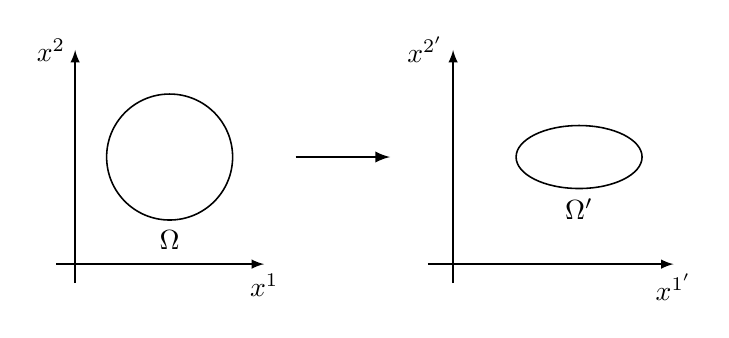
\begin{tikzpicture}[thick, scale=0.8]
    \draw[line width = 0.2mm] (0,0) circle (1cm);
    \draw[line width = 0.2mm] (6.5,0) ellipse (1cm and 0.5cm);
%    \draw[line width = 0.2mm] (11,0) ellipse (1cm and 0.5cm);
    \node[below, black] at (0,-1){$\Omega$};
    \node[below, black] at (6.5,-0.5){$\Omega '$};
%    \node[below, black] at (11,-0.5){$\Omega '$};
    \draw[line width = 0.2mm, black, ->, >=latex] (-1.8,-1.7)--(1.5,-1.7) node[below]{$x^{1}$};
    \draw[line width = 0.2mm, black, ->, >=latex] (-1.5,-2)--(-1.5,1.7) node[left]{$x^{2}$};
    \draw[line width = 0.2mm, black, ->, >=latex] (4.1,-1.7)--(8,-1.7) node[below]{$x^{1'}$};
    \draw[line width = 0.2mm, black, ->, >=latex] (4.5,-2)--(4.5,1.7) node[left]{$x^{2'}$};
%    \draw[line width = 0.2mm, black, ->, >=latex] (9,-1.7)--(12.9,-1.7) node[below]{$x^{1}$};
%    \draw[line width = 0.2mm, black, ->, >=latex] (9.4,-2)--(9.4,1.7) node[left]{$x^{2}$};
    \draw[line width = 0.3mm, black, ->, >=latex] (2,0)--(3.5,0);
%    \node[black] at (8.5,0){$=$};
    \end{tikzpicture}
    \caption{Ilustración esquemática de la transformación de la integral de acción invariante.}
    \label{Transformaciones}
\end{figure}
    
%----------------------------------------------------------------------------------------

\noindent
La variación de la densidad lagrangiana (\ref{2.39_a}) determina que la variación de la acción se escriba como
\begin{equation*}
\begin{split}
\delta S\left[ \phi \right] &=\int_{\Omega ^{\prime }}d^{4}x^{\prime }\left[ \mathcal{L}\left( \phi _{r}\left( x\right) ,\partial _{\mu }\phi _{r}\left(x\right) \right) +\delta \mathcal{L}\left( \phi _{r}\left( x\right),\partial _{\mu }\phi _{r}\left( x\right) \right) \right] -\int_{\Omega }d^{4}x\mathcal{L}\left( \phi _{r}\left( x\right) ,\partial _{\mu }\phi_{r}\left( x\right) \right) \\
&=\int_{\Omega ^{\prime }}d^{4}x^{\prime }\mathcal{L}\left( x\right)+\int_{\Omega ^{\prime }}d^{4}x^{\prime }\delta \mathcal{L}\left( x\right)-\int_{\Omega }d^{4}x\mathcal{L}\left( x\right) ~,
\end{split}
\end{equation*}
\noindent
donde se ha definido $\mathcal{L}\left( \phi_{r}\left( x\right) ,\partial _{\mu }\phi_{r}\left( x\right)\right)\equiv \mathcal{L}\left(x\right)$.\\

\noindent
Ahora, la transformación de coordenadas (\ref{2.36}) determina que el elemento de volumen de integración cambie en la siguiente forma,
\begin{equation}
d^{4}x^{\prime }=\left\vert \frac{\partial x^{\prime \mu }}{\partial x^{\nu }}\right\vert d^{4}x~,
\end{equation}
\noindent
siendo $\left\vert \frac{\partial x^{\prime \mu }}{\partial x^{\nu }}\right\vert$ el determinante Jacobiano de la transformación de coordenadas. Para hallar este determinante se parte de la expresión,
\begin{eqnarray}
\frac{\partial x^{\prime \mu }}{\partial x^{\nu }} &=&\frac{\partial }{%
\partial x^{\nu }}\left[ x^{\mu }+\delta x^{\mu }\right] =\frac{\partial
x^{\mu }}{\partial x^{\nu }}+\frac{\partial }{\partial x^{\nu }}\delta
x^{\mu }  \notag \\
&=&\delta _{\nu }^{\mu }+\partial _{\nu }\delta x^{\mu }~,
\end{eqnarray}
\noindent
de manera que al considerar aproximaciones a primer orden,
 
\begin{eqnarray}
\left\vert \frac{\partial x^{\prime \mu }}{\partial x^{\nu }}\right\vert 
&=&\left\vert \delta _{\nu }^{\mu }+\partial _{\nu }\delta x^{\mu
}\right\vert   \notag \\
&=&\left\vert 
\begin{array}{cccc}
\delta _{0}^{0}+\partial _{0}\delta x^{0} & \delta _{1}^{0}+\partial
_{1}\delta x^{0} & \cdots  & \cdots  \\ 
\delta _{0}^{1}+\partial _{0}\delta x^{1} & \delta _{1}^{1}+\partial
_{1}\delta x^{1} & \cdots  & \cdots  \\ 
\vdots  & \vdots  & \ddots  & \vdots  \\ 
\cdots  & \cdots  & \cdots  & \delta _{3}^{3}+\partial _{3}\delta x^{3}%
\end{array}%
\right\vert   \notag \\
&=&\left\vert 
\begin{array}{cccc}
1+\partial _{0}\delta x^{0} & \partial _{1}\delta x^{0} & \cdots  & \cdots 
\\ 
\partial _{0}\delta x^{1} & 1+\partial _{1}\delta x^{1} & \cdots  & \cdots 
\\ 
\vdots  & \vdots  & \ddots  & \vdots  \\ 
\cdots  & \cdots  & \cdots  & 1+\partial _{3}\delta x^{3}
\end{array}%
\right\vert   \notag \\
&\approx &\left( 1+\partial _{0}\delta x^{0}\right) \left( 1+\partial_{1}\delta x^{2}\right) \left( 1+\partial _{2}\delta x^{2}\right) \left(1+\partial _{3}\delta x^{3}\right)   \notag \\
&\approx &1+\partial _{0}\delta x^{0}+\partial _{1}\delta x^{2}+\partial_{2}\delta x^{2}+\partial _{3}\delta x^{3}  \notag \\
&=&1+\partial _{\mu }\delta x^{\mu }~,
\end{eqnarray}

\noindent
de tal manera que
\begin{equation}
\begin{split}
        d^{4}x^{\prime}&=\left(1+\partial _{\mu }\delta x^{\mu } \right)d^{4}x \\
        &=d^{4}x+d^{4}x\partial _{\mu }\delta x^{\mu }~.
\end{split}
\end{equation}

\noindent
Con base en este resultado la variación de la acción se escribe
\begin{eqnarray}
\delta S[\phi ] &=&\int_{\Omega }\left( d^{4}x+d^{4}x\partial _{\mu }\delta x^{\mu }\right) \mathcal{L}\left( x\right) +\int_{\Omega }\left(d^{4}x+d^{4}x\partial _{\mu }\delta x^{\mu }\right) \delta \mathcal{L}\left(x\right) -\int_{\Omega }d^{4}x\mathcal{L}\left( x\right)   \notag \\
&\approx &\int_{\Omega }d^{4}x\partial _{\mu }\delta x^{\mu }\mathcal{L} \left( x\right) +\int_{\Omega }d^{4}x\delta \mathcal{L}\left( x\right) ~.
\end{eqnarray}
Expresando ahora la variación de la acción en términos de la variación total de la densidad Lagrangiana, la relación (\ref{2.38_aa}) implica 
\begin{equation}
\delta \mathcal{L}\left( x\right) =\tilde{\delta}\mathcal{L}\left( x\right)
+\delta x^{\mu }\partial _{\mu }\mathcal{L}\left( x\right) ~,
\end{equation}
lo que conlleva a deducir:

\begin{eqnarray}
\delta S\left[ \phi \right]  &=&\int_{\Omega }d^{4}x\partial _{\mu }\delta
x^{\mu }\mathcal{L}\left( x\right) +\int_{\Omega }d^{4}x\tilde{\delta}\mathcal{%
L}\left( x\right) +\int_{\Omega }d^{4}x\delta x^{\mu }\partial _{\mu }%
\mathcal{L}\left( x\right)   \notag \\
&=&\int_{\Omega }d^{4}x\partial _{\mu }\left[ \delta x^{\mu }\mathcal{L}%
\left( x\right) \right] +\int_{\Omega }d^{4}x\tilde{\delta}\mathcal{L}\left(
x\right) 
\end{eqnarray}
pero, al expresar la variaci\'{o}n total de la densidad Lagrangiana en t\'{e}rminos de la variaci\'{o}n de los campos y sus derivadas resulta,
\begin{eqnarray*}
\tilde{\delta}\mathcal{L}\left( x\right)  &=&\frac{\partial \mathcal{L}\left(
x\right) }{\partial \phi _{r}}\tilde{\delta}\phi _{r}+\frac{\partial \mathcal{L%
}\left( x\right) }{\partial \left( \partial _{\nu }\phi _{r}\right) }\tilde{%
\delta}\left( \partial _{\nu }\phi _{r}\right) ~,~\ \ \ \ \ \ \ \left[
\partial _{\mu },\tilde{\delta}\right] =0 \\
&=&\frac{\partial \mathcal{L}\left( x\right) }{\partial \phi _{r}}\tilde{\delta%
}\phi _{r}+\frac{\partial \mathcal{L}\left( x\right) }{\partial \left(
\partial _{\nu }\phi _{r}\right) }\partial _{\nu }\tilde{\delta}\phi _{r} \\
&=&\left[ \frac{\partial \mathcal{L}\left( x\right) }{\partial \phi _{r}}%
-\partial _{\nu }\frac{\partial \mathcal{L}\left( x\right) }{\partial \left(
\partial _{\nu }\phi _{r}\right) }\right] \tilde{\delta}\phi _{r}+\frac{%
\partial \mathcal{L}\left( x\right) }{\partial \left( \partial _{\nu }\phi
_{r}\right) }\partial _{\nu }\tilde{\delta}\phi _{r}+\partial _{\nu }\frac{%
\partial \mathcal{L}\left( x\right) }{\partial \left( \partial _{\nu }\phi
_{r}\right) }\tilde{\delta}\phi _{r} \\
&=&\left[ \frac{\partial \mathcal{L}\left( x\right) }{\partial \phi _{r}}%
-\partial _{\nu }\frac{\partial \mathcal{L}\left( x\right) }{\partial \left(
\partial _{\nu }\phi _{r}\right) }\right] \tilde{\delta}\phi _{r}+\partial
_{\nu }\left[ \frac{\partial \mathcal{L}\left( x\right) }{\partial \left(
\partial _{\nu }\phi _{r}\right) }\tilde{\delta}\phi _{r}\right] ~,
\end{eqnarray*}
\noindent
resultado que permite expresar la variaci\'{o}n total de la acci\'{o}n como
\begin{eqnarray*}
\delta S\left[ \phi \right]  &=&\int_{\Omega }d^{4}x\partial _{\mu }\left[\delta x^{\mu }\mathcal{L}\left( x\right) \right] +\int_{\Omega}d^{4}x\left\{ \left[ \frac{\partial \mathcal{L}\left( x\right) }{\partial \phi _{r}}-\partial _{\nu }\frac{\partial \mathcal{L}\left( x\right) }{\partial \left( \partial _{\nu }\phi _{r}\right) }\right] \tilde{\delta}\phi
_{r}+\partial _{\nu }\left[ \frac{\partial \mathcal{L}\left( x\right) }{\partial \left( \partial _{\nu }\phi _{r}\right) }\tilde{\delta}\phi _{r}\right] \right\}  \\
&=&\int_{\Omega }d^{4}x\partial _{\mu }\left[ \delta x^{\mu }\mathcal{L}\left( x\right) +\frac{\partial \mathcal{L}\left( x\right) }{\partial \left(\partial _{\mu }\phi _{r}\right) }\tilde{\delta}\phi _{r}\right] +\int_{\Omega}d^{4}x \left[ \frac{\partial \mathcal{L}\left( x\right) }{\partial \phi _{r}}-\partial _{\nu }\frac{\partial \mathcal{L}\left( x\right) }{\partial \left( \partial _{\nu }\phi _{r}\right) }\right] \tilde{\delta}\phi_{r} ~,
\end{eqnarray*}
al escribir la variación total del campo $\phi_{r}$ con base en (\ref{2.38_aa}), la expresión anterior se transforma en,

\begin{eqnarray}
\delta S\left[ \phi \right]  &=&\int_{\Omega }d^{4}x~\partial _{\mu }\left[ \frac{\partial \mathcal{L}\left( x\right) }{\partial \left( \partial _{\mu}\phi _{r}\right) }\left( \delta \phi _{r}-\delta x^{\nu }\partial _{\nu
}\phi _{r}\left( x\right) \right) +\delta x^{\mu }\mathcal{L}\left( x\right) \right]   \notag \\
&&+\int_{\Omega }d^{4}x\left[ \frac{\partial \mathcal{L}\left( x\right) }{\partial \phi _{r}}-\partial _{\nu }\frac{\partial \mathcal{L}\left(x\right) }{\partial \left( \partial _{\nu }\phi _{r}\right) }\right] \tilde{\delta}\phi _{r}  \notag \\
&=&\int_{\Omega }d^{4}x~\left\{ \partial _{\mu }\left[ \frac{\partial \mathcal{L}\left( x\right) }{\partial \left( \partial _{\mu }\phi_{r}\right) }\delta \phi _{r}-\delta x^{\nu }\left( \frac{\partial \mathcal{L%
}\left( x\right) }{\partial \left( \partial _{\mu }\phi _{r}\right) }\partial _{\nu }\phi _{r}\left( x\right) -g_{~\nu }^{\mu }\mathcal{L}\left(x\right) \right) \right] \right.   \notag \\
&&+\left. \left[ \frac{\partial \mathcal{L}\left( x\right) }{\partial \phi_{r}}-\partial _{\nu }\frac{\partial \mathcal{L}\left( x\right) }{\partial\left( \partial _{\nu }\phi _{r}\right) }\right] \tilde{\delta}\phi_{r}\right\} ~.
\end{eqnarray}

\noindent
Aquí se debe recordar lo planteado en la definición (\ref{definoether}) de simetría, en la cual ante las transformaciones (\ref{2.36}) y (\ref{2.37}) se debe garantizar la coovarianza de la densidad Lagrangiana y que la acción permanezca invariante, de manera que

\begin{equation}
    \delta S \left[\phi \right] = 0~,
\end{equation}
lo que conlleva a
\begin{equation}
    \begin{split}
    \delta S \left[\phi \right] &=\int_{\Omega }d^{4}x~\left\{ \partial _{\mu }\left[ \frac{\partial \mathcal{L}\left( x\right) }{\partial \left( \partial _{\mu }\phi_{r}\right) }\delta \phi _{r}-\delta x^{\nu }\left( \frac{\partial \mathcal{L}\left( x\right) }{\partial \left( \partial _{\mu }\phi _{r}\right) } \partial _{\nu }\phi _{r}\left( x\right) -g_{~\nu }^{\mu }\mathcal{L}\left(x\right) \right) \right] \right.   \\
    &+\left. \left[ \frac{\partial \mathcal{L}\left( x\right) }{\partial \phi_{r}}-\partial _{\nu }\frac{\partial \mathcal{L}\left( x\right) }{\partial \left( \partial _{\nu }\phi _{r}\right) }\right] \tilde{\delta}\phi_{r}\right\}=0 ~. \label{vaccion}
    \end{split}
\end{equation}

\noindent
Se debe tener presente que el volumen de integración $\Omega$ es completamente arbitrario, por ende el integrando de (\ref{vaccion}) deberá desaparecer si la acción es invariante por las transformaciones consideradas, de modo que se debe cumplir:
\begin{equation}
    \partial_{\mu}f^{\mu}(x)+\left( \frac{\partial \mathcal{L}\left( x\right) }{\partial \phi_{r}}-\partial _{\nu }\frac{\partial \mathcal{L}\left( x\right) }{\partial \left( \partial _{\nu }\phi _{r}\right) }\right)\bar{\delta}\phi_{r}=0~,
    \label{intcero}
\end{equation}
\noindent
donde se define el campo vectorial dependiente de las coordenadas,
\begin{equation}
\boxed{
    f^{\mu}(x) \equiv \frac{\partial \mathcal{L}\left( x\right) }{\partial \left( \partial _{\mu }\phi_{r}\right) }\delta \phi _{r}(x)-\delta x^{\nu }\left( \frac{\partial \mathcal{L}\left( x\right) }{\partial \left( \partial _{\mu }\phi _{r}\right) } \partial _{\nu }\phi _{r}\left( x\right) -g_{~\nu }^{\mu }\mathcal{L}\left(x\right) \right)~,
    \label{fmu}
    }
\end{equation}

\noindent
Si los campos que describen el sistema $\phi_{r}(x)$ satisfacen las ecuaciones de movimiento Euler-Lagrange, el segundo término entre paréntesis de la relación (\ref{intcero}) desaparece, de modo que se obtiene,
\begin{equation}
\boxed{
    \partial_{\mu}f^{\mu}(x)=0~,
    }
\end{equation}
\noindent
Esta expresión representa la \textbf{ecuación de continuidad} para el campo vectorial $f^{\mu}(x)$ que se lo identificará como una \emph{``densidad de corriente''} o \emph{``corriente de Noether''}. Esta ecuación garantizará la existencia de una ley de conservación expresada en forma de ecuación diferencial. Con el fin de observar esto, se integra la ecuación de continuidad sobre el espacio tridimensional, de manera que 

\begin{eqnarray*}
0 &=&\int_{V}d^{3}x~\partial _{\mu }f^{\mu }\left( x\right)
=\int_{V}d^{3}x~\partial _{0}f^{0}\left( x\right) +\int_{V}d^{3}x~\partial_{i}f^{i}\left( x\right)  \\
&=&\int_{V}d^{3}x~\frac{\partial f^{0}\left( x\right) }{\partial x^{0}}+\int_{V}d^{3}x~\partial _{i}f^{i}\left( x\right)  \\
&=&\frac{d}{dx^{0}}\int_{V}d^{3}x~f^{0}\left( x\right) +\int_{V}d^{3}x\div{\vb{f\left( x\right)}}  \\
&=&\frac{d}{dx^{0}}\int_{V}d^{3}x~f^{0}\left( x\right) +\oint_{\mathcal{S}}d\vb{a}\vdot\vb{f}\left(x\right) ~,
\end{eqnarray*}

\noindent
donde se ha utilizado el teorema de la divergencia. Teniendo en cuenta que los campos $\phi_{r}(x)$ y sus derivadas desaparecen sobre la superficie $\mathcal{S}$ que limita al volumen $V$ (que tiende a infinito), la segunda integral de la relación anterior desaparece lo que genera el resultado,
\begin{equation*}
    \frac{d}{dx^{0}}\int_{V}d^{3}x~f^{0}\left( x\right)=\frac{d}{dt}\int_{V}d^{3}x~f^{0}\left( x\right)=0~,
\end{equation*}

\noindent
este resultado permite establecer una carga que se conserva en el tiempo, definida de la forma 
\begin{equation}
\begin{split}
    Q &\equiv \int_{V}d^{3}x~f^{0}\left( x\right) \\ 
    &=\int_{V}d^{3}x~\left\{ \frac{\partial \mathcal{L}\left( x\right) }{\partial \left( \partial _{0 }\phi_{r}\right) }\delta \phi _{r}(x)-\delta x^{\nu }\left( \frac{\partial \mathcal{L}\left( x\right) }{\partial \left( \partial _{0}\phi _{r}\right) } \partial _{\nu }\phi _{r}\left( x\right) -g_{~\nu }^{0 }\mathcal{L}\left(x\right) \right)\right\}~.
    \label{carganoether}
\end{split}
\end{equation}
\noindent
En la literatura (\ref{carganoether}) se denomina carga de Noether y es la expresión que se empleará para determinar la carga conservada bajo diferentes simetrías. Cada uno de los resultados obtenidos se enuncian en el siguiente teorema.

\begin{theorem}[Primer Teorema de Noether]
Cada transformación de simetría continua conduce a una ley de conservación donde la cantidad conservada $Q$ se puede obtener de la densidad Lagrangiana asociada al sistema mediante las expresiones (\ref{fmu}) y (\ref{carganoether}).
\end{theorem}

\vspace{0.4cm}
\subsection{Aplicaciones del Teorema de Noether}
\vspace{0.2cm}

Supongamos que tenemos una transformación infinitesimal, que se escribe en términos de ciertos parámetros $\epsilon^{a}$, que cambia las coordenadas y los campos de la siguiente manera

\begin{eqnarray}
x^{\mu } &\rightarrow &x^{\prime \mu }=x^{\mu }+\delta x^{\mu }\equiv x^{\mu}+\epsilon ^{a}A_{a}^{\mu }\left( x\right) \label{xmue} \\
\phi _{r}\left( x\right)  &\rightarrow &\phi _{r}^{\prime }\left( x^{\prime}\right) =\phi _{r}\left( x\right) +\delta \phi _{r}\left( x\right) \equiv \phi_{r}\left( x\right) +\epsilon ^{a}F_{r,a}\left( x \right) \label{fmue} ,
\end{eqnarray}
\noindent
El índice $a$ etiqueta la cantidad de parámetros infinitesimales, mientras que el índice $r$ el número de campos. Decimos que esta transformación es una simetría si deja invariante la acción.  En dicho caso, el teorema de Noether asegura que
%si hay más de uno o de componentes del campo si el mismo es por ejemplo un espinor de Dirac. 
\begin{equation}
    \partial_{\mu} f^{\mu}_{a}=0~,
\end{equation}
sobre las soluciones de las ecuaciones de movimiento, siendo
\begin{equation}
f^{\mu }(x)=\epsilon^{a}\frac{\partial \mathcal{L}\left( x\right) }{\partial \left(
\partial _{\mu }\phi _{r}\right) }\left[ F_{r,a}\left( x\right) -A_{a}^{\nu
}\left( x\right) \partial _{\nu }\phi _{r}\left( x\right) \right]
+\epsilon^{a} A_{a}^{\mu }\left( x\right) \mathcal{L}\left( x\right) ~.
\end{equation}
Además, la cantidad
\begin{equation}
    Q=\int \dd[3]{x} x f^{0}(x)~,
    \label{eq_2.100}
\end{equation}

\noindent
es una constante de movimiento,  es decir, no cambia en el tiempo (sobre las soluciones de las ecuaciones de movimiento).\\

\noindent
Para entender el teorema y cómo usarlo, se empieza con un ejemplo. Comencemos viendo el caso en el cual se tiene invariancia ante traslaciones.


\subsection{Invarianza ante traslaciones Espacio-Temporales}
La invariancia bajo traslaciones es caracterizada por las siguientes transformaciones en las coordenadas y campos:

%\begin{equation}
%\begin{split}
%    x^{\prime \mu}&=x^{\mu}+\epsilon^{\mu}\\
%    &=x^{\mu}+\epsilon^{\nu}g^{\mu}_{~\nu}~,~~~~~\therefore~~~~\delta x^{\mu}=\epsilon^{\mu}~,
%    \label{xpmut}
%\end{split}
%\end{equation}

\begin{equation}
\begin{split}
x^{\mu } \longmapsto x^{\prime \mu } & = x^{\mu }+\epsilon ^{\mu }~\ \implies \epsilon ^{a}=\epsilon ^{\nu }~;~A_{a}^{\mu }=\delta _{\nu }^{\mu } \\
\phi _{r}\left( x\right)  \longmapsto ~\phi _{r}^{\prime }\left( x^{\prime}\right) & = \phi_{r}\left( x^{\prime }-\epsilon \right) = \phi _{r}\left(x\right) ~\ \implies F_{r,a}=F_{r,\mu }=0.
\label{xpmut}
\end{split}
\end{equation}
\noindent

siendo $\epsilon_{\mu}$ un cuadrivector constante\footnote{Note que según la ecuación (\ref{xmue}), en este caso $A^{\mu}_{\nu}=g^{\mu}_{~\nu}$ y se identifica el índice $a \rightarrow \mu$, porque hay cuatro traslaciones infinitesimales, una por cada dirección del espacio-tiempo.}.

%el cual induce la siguiente transformación en los campos: 

%\begin{equation}
%\phi _{r}\left( x\right) \rightarrow \phi ^{\prime }_{r}\left( x^{\prime}\right) =\phi_{r}\left( x^{\prime %}-\epsilon \right) =\phi_{r}\left( x\right) ~,
%\label{ftr}
%\end{equation}

Observe que la invariancia por traslaciones espacio temporales son consecuencia de la homogeneidad del espacio-tiempo donde la forma del campo es supuesta para no cambiar por traslaciones, por ende las variaciones locales de los campos son nulas\footnote{El hecho que la variación en los campos sea nula implica que la cantidad dada en (\ref{fmue}) sea nula, es decir $F_{r,\mu}=0$.}

%\begin{equation}
%    \delta \phi_{r}(x)=0~.
%    \label{vfitr}
%\end{equation}

\noindent
Hasta aquí, lo único que hicimos fue ver qué sucede con las coordenadas y los campos ante una traslación. Para poder aplicar el teorema de Noether, necesitamos ver si esta es una transformación de simetría, es decir, si deja invariante la acción. En este caso, mostrar esto es sencillo, ya que el mismo Lagrangiano queda invariante, puesto que 

\begin{equation}
    \mathcal{L}^{\prime}\left(x^{\prime}\right) \equiv \mathcal{L}\left[\phi^{\prime}\left(x^{\prime}\right), \frac{\partial \phi^{\prime}}{\partial x^{\prime}}, x^{\prime}\right]=\mathcal{L}\left[\phi(x), \frac{\partial \phi}{\partial x^{\prime}}, x^{\prime}\right]~,
\end{equation}
\noindent
pero como $\epsilon^{\mu}$ es un cuadrivector constante, derivar respecto a $x^{\prime}$ es lo mismo que derivar respecto a $x$, por lo que
\begin{equation}
    \mathcal{L}^{\prime}\left(x^{\prime}\right)=\mathcal{L}\left[\phi(x), \frac{\partial \phi}{\partial x}, x^{\prime}\right]~,
\end{equation}

\noindent
El último término en el corchete, $x^{\prime}$, está puesto porque podría pasar que el Lagrangiano dependiera explícitamente de las coordenadas. En nuestro estudio, se verá que la única dependencia del Lagrangiano en las coordenadas aparece sólo a través de los campos, de modo que podemos obviar eso. De este modo, resulta
\begin{equation}
    \mathcal{L}^{\prime}\left(x^{\prime}\right)=\mathcal{L}\left[\phi(x), \frac{\partial \phi}{\partial x}\right]=\mathcal{L}(x),
\end{equation}
y como $d^{4} x^{\prime}=d^{4} x$ la acción también es invariante. Esto nos dice que las traslaciones son simetrías y entonces hay corrientes conservadas. Recurriendo a la ecuación (\ref{fmu}) y reemplazando las transformaciones (\ref{xpmut}):
%y (\ref{vfitr}):

\begin{equation}
f^{\mu }(x)=-\epsilon ^{\nu }\left( \frac{\partial \mathcal{L}\left(x\right) }{\partial \left( \partial _{\mu }\phi _{r}\right) }\partial _{\nu}\phi _{r}\left( x\right) -g_{~\nu }^{\mu }\mathcal{L}\left( x\right)\right) ~,
\end{equation}

\noindent
de tal manera que la ecuación de continuidad tendrá la siguiente forma
\begin{equation}
    \begin{split}
        \partial_{\mu}f^{\mu}&=\partial_{\mu} \left\{ -\epsilon ^{\nu }\left( \frac{\partial \mathcal{L}\left(x\right) }{\partial \left( \partial _{\mu }\phi _{r}\right) }\partial _{\nu}\phi _{r}\left( x\right) -g_{~\nu }^{\mu }\mathcal{L}\left( x\right)\right) \right\} \\
        &=-\epsilon ^{\nu } \partial_{\mu} \left\{ \left( \frac{\partial \mathcal{L}\left(x\right) }{\partial \left( \partial _{\mu }\phi _{r}\right) }\partial _{\nu}\phi _{r}\left( x\right) -g_{~\nu }^{\mu }\mathcal{L}\left( x\right)\right) \right\}~,
    \end{split}
\end{equation}

\noindent
siendo $\epsilon^{\mu}$ constante, la ecuación de continuidad asociada esta simetría tendrá la forma
\begin{equation}
    \partial_{\mu} \Theta^{\mu}_{~\nu}=0,
    \label{derThe}
\end{equation}
donde se ha definido la siguiente corriente de Noether:
\begin{equation}
\boxed{
    \Theta^{\mu}_{~\nu}\equiv  \frac{\partial \mathcal{L}\left(x\right) }{\partial \left( \partial _{\mu }\phi _{r}\right) }\partial _{\nu}\phi _{r}\left( x\right) -g_{~\nu }^{\mu }\mathcal{L}\left( x\right)~,
    \label{TME}
    }
\end{equation}

\noindent
La relación (\ref{TME}) establece que la corriente de Noether es un tensor de segundo orden y se lo conoce como \emph{tensor canónico de momento-energía}. De la ecuación (\ref{carganoether}) se determina que la correspondiente carga de Noether se deriva cuando $\mu=0$, es decir

\begin{equation}
    Q^{\nu}=\int_{V} d^{3}x \Theta^{0 \nu}(x) \equiv P^{\nu}~,
    \label{eq_2.109}
\end{equation}

\noindent    
de ahí que
\begin{equation}
        Q^{\nu}= \int_{V} d^{3}x \left[ \frac{\partial \mathcal{L}\left(x\right) }{\partial \left( \partial _{0 }\phi _{r}\right) }\partial ^{\nu}\phi _{r}\left( x\right) -g^{0 \nu }\mathcal{L}\left( x\right) \right]~.
\end{equation}

\noindent
Del hecho que $\nu=0,1,2,3$ se determina que existen cuatro cantidades conservadas asociadas a esta simetría y que se identifican como la energía $E$, y el momentum $\mathbf{P}$ del campo, que en notación cuadri-dimensional se expresa en la forma (en unidades naturales)
\begin{equation}
    P^{\nu}=\left(E,\mathbf{P}\right)=\int_{V} d^{3}x \Theta ^{0 \nu} =\text{constante}~.
    \label{PnuT}
\end{equation}

\noindent
De las relaciones (\ref{TME}) y (\ref{PnuT}) se puede determinar que la energía del sistema es
\begin{eqnarray}
E &=&\int_{V}d^{3}x\Theta ^{00}\left( x\right)   \notag \\
&=&\int_{V}\left( \frac{\partial \mathcal{L}\left( x\right) }{\partial \left( \partial _{0}\phi _{r}\right) }\partial ^{0}\phi _{r}\left( x\right)-g^{00}\mathcal{L}\left( x\right) \right)   \notag \\
&=&\int_{V}\left( \frac{\partial \mathcal{L}\left( x\right) }{\partial \dot{\phi}_{r}}\dot{\phi}_{r}\left( x\right)-\mathcal{L}\left( x\right) \right) ~,
\end{eqnarray}
 
 la cual corresponde al Hamiltoniano canónico asociado al sistema y $\Theta^{00}$ es la correspondiente densidad hamiltoniana canónica. (Ver ecuaciones (\ref{HC}) y (\ref{dHC}))\\
  
Observe que el tensor $\Theta^{\mu \nu}$ definido en (\ref{TME}) en algunos casos resulta no ser simétrico. Sin embargo, es posible pasar a un tensor de momento-energía simétrico $T^{\mu \nu}=T^{\nu \mu}$ conocido como tensor de \emph{Belinfante}, agregando un término adecuado que tenga cuadridivergencia nula. El nuevo tensor también satisface la ley de conservación (\ref{derThe}) y genera el mismo $P^{\mu}$.\\
 
 \noindent
Podemos usar esta libertad para construir un tensor de momento-energía que sea simetríco, para ello se define:
 
\begin{equation}
T^{\mu \nu }=\Theta ^{\mu \nu }+\partial _{\sigma }\chi ^{\sigma \mu \nu }~,
\end{equation}%
donde $\chi _{\sigma \mu \nu }$ es un tensor arbitrario antisim\'{e}trico en
sus dos primeros \'{\i}ndices, es decir%
\begin{equation}
\chi ^{\sigma \mu \nu }=-\chi ^{\mu \sigma \nu }~,
\end{equation}

ya que esta condición nos asegura que tenga divergencia nula y que entonces $T^{\mu \nu }$ también será una corriente conservada. En efecto


\begin{eqnarray*}
\partial _{\mu }T^{\mu \nu } &=&\partial _{\mu }\Theta ^{\mu \nu }+\partial
_{\mu }\partial _{\sigma }\chi ^{\sigma \mu \nu } \\
&=&\partial _{\mu }\Theta ^{\mu \nu }+\frac{1}{2}\left( \partial _{\mu
}\partial _{\sigma }\chi ^{\sigma \mu \nu }+\partial _{\mu }\partial
_{\sigma }\chi ^{\sigma \mu \nu }\right)  \\
&=&\partial _{\mu }\Theta ^{\mu \nu }+\frac{1}{2}\left( \partial _{\mu
}\partial _{\sigma }\chi ^{\sigma \mu \nu }+\partial _{\sigma }\partial
_{\mu }\chi ^{\mu \sigma \nu }\right) 
\end{eqnarray*}%
donde $\partial _{\mu }\partial _{\sigma }$ es un tensor sim\'{e}trico en
los \'{\i}ndices $\mu ,\sigma $ dado que,%
\begin{equation*}
S_{\mu \sigma }\equiv \partial _{\mu }\partial _{\sigma }=\frac{\partial }{%
\partial x^{\mu }}\frac{\partial }{\partial x^{\sigma }}=\frac{\partial ^{2}%
}{\partial x^{\mu }\partial x^{\sigma }}=\frac{\partial ^{2}}{\partial
x^{\sigma }\partial x^{\mu }}=\frac{\partial }{\partial x^{\sigma }}\frac{%
\partial }{\partial x^{\mu }}=\partial _{\sigma }\partial _{\mu }=S_{\sigma
\mu }~,
\end{equation*}%
por lo tanto,
\begin{eqnarray*}
\partial _{\mu }T^{\mu \nu } &=&\partial _{\mu }\Theta ^{\mu \nu }+\frac{1}{2%
}\partial _{\mu }\partial _{\sigma }\underset{\chi ^{\sigma \mu \nu }-\chi
^{\sigma \mu \nu }=0}{\underbrace{\left( \chi ^{\sigma \mu \nu }+\chi ^{\mu
\sigma \nu }\right) }} \\
&=&\partial _{\mu }\Theta ^{\mu \nu } =0~,
\end{eqnarray*}

\noindent
verificándose además que $T^{\mu \nu}$ y $\Theta^{\mu \nu}$ tienen las mismas cargas conservadas.\\

En conclusión, la invariancia bajo traslaciones espacio-temporales implica la conservación del cuadrimomento, $P^{\mu}$.


\vspace{1cm}

\subsection{Invarianza de Lorentz o ante rotaciones y boots}

\vspace{0.3cm}

Se ha estudiado como el espacio-tiempo es homogéneo ante traslaciones espacio-temporales, ahora se considerará isótropo ante rotaciones, por lo tanto, la acción que se requiere debe ser invariante bajo transformaciones de Lorentz. Estas trasformaciones incluyen además de las usuales rotaciones en el espacio tridimensional, transformaciones en la velocidad (\emph{Boosts de Lorentz}), que se interpretan como rotaciones en el espacio-tiempo.\\

\noindent
La rotación infinitesimal más general se expresa como:
\begin{equation}
    x^{\prime}_{\mu}=x_{\mu}+\delta\omega_{\mu}^{~\nu} x_{\nu}.
\end{equation}

%\implies \epsilon^{a} = \omega^{\mu \nu}
%de manera que $\delta x_{\mu}=x^{\prime}_{\mu}-x_{\mu}=\delta \omega_{\mu}^{~\nu}x_{\nu}$.\\

La cantidad $\delta \omega^{\mu \nu}$ dependiente de los ángulos de rotación en el espacio tiempo.
Para garantizar la invariancia en la magnitud del vector $x^{\mu}$ ante una rotación en el espacio de Minkowski, el tensor $\omega^{\mu \nu}$ debe ser antisimétrico. Para ver esto partimos de la condición

\begin{equation}
    x^{\prime 2}=x^{2}~\implies ~g_{\mu \nu }x^{\prime \mu }x^{\prime \nu
}=g_{\alpha \beta }x^{\alpha }x^{\beta },
\end{equation}

donde

\begin{equation}
    \begin{split}
    g_{\mu \nu }x^{\prime \mu }x^{\prime \nu } & = g_{\mu \nu }\left( x^{\mu}+\delta \omega ^{\mu \alpha }x_{\alpha }\right) \left( x^{\nu }+\delta \omega ^{\nu \beta }x_{\beta }\right)  \\
    & \approx g_{\mu \nu }x^{\mu }x^{\nu }+2\delta \omega ^{\mu \nu }x_{\mu}x_{\nu }.
    \end{split}
    \label{eq2.117}
\end{equation}

la ecuación (\ref{eq2.117}) se garantiza si $\delta \omega ^{\mu \nu }x_{\mu}x_{\nu}$ se anula. Para satisfacer esta afirmación se debe cumplir que
\begin{equation}
    \delta \omega ^{\mu \nu }x_{\mu }x_{\nu } = \frac{1}{2}\left( \omega ^{\mu \nu}+\omega ^{\nu \mu }\right) x_{\mu }x_{\nu }+\cancelto{0}{ \frac{1}{2}\left( \omega ^{\mu \nu }-\omega ^{\nu \mu }\right) x_{\mu }x_{\nu }}=0,
    \label{eq2.118}
\end{equation}

pero el tensor $x_{\mu}x_{\nu}$ es simetrico en sus índices $\mu \nu$, por lo tanto el segundo término resulta ser el producto de un tensor simétrico con otro antisimétrico hecho que hace cero dicho término. Por tanto la expresión (\ref{eq2.118}) se garantiza si $\delta \omega ^{\mu \nu }$ es un tensor completamente antisimétrico. 

\begin{equation}
    \delta \omega ^{\mu \nu }=-\delta \omega ^{\nu \mu  }.
    \label{eq2.119}
\end{equation}

Para ver la manera en como transforman los campos se propone que los campos transformados muestren una dependencia lineal sobre los ángulos de rotación presentes en el tensor $\delta \omega ^ {\mu \nu}$ y sobre los campos mismos $\phi_{r}(x)$. Esta dependencia se la propone a partir del siguiente ansatz:

\begin{equation}
    \phi _{r}^{\prime }\left( x^{\prime }\right) =\phi _{r}\left( x\right) + \frac{1}{2}\delta \omega _{\mu \nu }\left( I^{\mu \nu }\right) _{rs}\phi _{s}\left( x\right) ~~~ \implies~~~ \delta \phi_{r}(x) = \frac{1}{2}\delta \omega_{\mu \nu }\left( I^{\mu \nu }\right) _{rs}\phi _{s}\left( x\right) .
    \label{eq2.120}
\end{equation}

En esta expresión se debe tener presente que los campos $\phi_{r}(x)$ transforman de acuerdo a una representación \emph{irreducible del grupo de Lorentz}, por tanto $(I^{\mu \nu})_{ij}$ son elementos de matriz correspondientes al generador infinitesimal\footnote{Estos generadores son la representación de los elementos del grupo de Lorentz sobre el espacio vectorial generado por los campos $\phi$. Un análisis exhaustivo se halla en el apéndice \ref{Apendice_A}.}. Las Cantidades $I^{\mu \nu}$ se identifican como \emph{generadores infinitesimales de la transformación de Lorentz}, tensor de segundo orden que se caracteriza por ser antisimétrico, consecuencia de (\ref{eq2.119}). De este modo $I^{\mu \nu}$ tendrá asociados seis componentes independientes:

\begin{equation}
    \begin{split}
        (\mu,\nu) &= (1,2);(1,3);(2,3)~~\longmapsto ~\text{Rotaciones espaciales}\\
        (\mu,\nu) &= (0,1);(0,2);(0,3)~~\longmapsto ~\text{Boost de Lorentz}.\\
    \end{split}
\end{equation}

Al ser $I^{\mu \nu}$ un conjunto de generadores infinitesimales del grupo de Lorentz en el álgebra de Lie, se satisface la relación de anticonmutación:
\begin{equation*}
    \comm{I^{\mu \nu}}{I^{\sigma \tau}}=g^{\nu \sigma}I^{\sigma \tau}+g^{\mu \tau}I^{\nu \sigma} - g^{\nu \tau}I^{\mu \sigma}-g^{\mu \sigma}I^{\nu \tau}.
\end{equation*}
Por tanto, esta álgebra de Lie define la estructura de grupo de Lorentz y es válida en cualquer representación.\\

Ahora, la corriente de Noether (ver (\ref{fmu})) asociada a esta simetría es:

\begin{equation}
    \begin{split}
    f^{\mu}(x) &= \pdv{\mathcal{L}}{(\partial_{\mu}\phi_{r})} \qty[\frac{1}{2} \delta \omega_{\alpha \beta} \qty(I^{\alpha \beta})_{rs}\phi_{s}(x)]-\delta \omega^{\nu \alpha}x_{\alpha} \qty[\pdv{\mathcal{L}}{(\partial_{\mu}\phi_{r})}\partial_{\nu}\phi_{r}(x)-g^{\mu}_{~\nu}\mathcal{L}(x)]\\
    &= \frac{1}{2} \pdv{\mathcal{L}}{(\partial_{\mu}\phi_{r})}\delta \omega_{\alpha \beta} \qty(I^{\alpha \beta})_{rs}\phi_{s}(x)-\Theta^{\mu}_{\nu}\delta x^{\alpha} \omega_{\nu \alpha}
    \end{split}
    \label{eq2.122}
\end{equation}

donde se ha empleado la definición del tensor energía-momento (\ref{TME}). Sin embargo, se puede realizar una antisimetrización en el tensor $\Theta^{\mu \nu}x^{\alpha}$ empleando \ref{eq2.119}, de la siguiente manera:

\begin{equation}
    \begin{split}
        \Theta ^{\mu \nu }x^{\alpha }\delta \omega _{\nu \alpha } &= \cancelto{0}{
        \frac{1}{2} \qty(\Theta ^{\mu \nu }x^{\alpha }+\Theta ^{\mu \alpha }x^{\nu })\delta \omega_{\nu \alpha }}+\frac{1}{2} \qty(\Theta ^{\mu \nu }x^{\alpha }-\Theta ^{\mu \alpha}x^{\nu })\delta \omega _{\nu \alpha } \\
        &= \frac{1}{2}(\Theta ^{\mu \nu }x^{\alpha }-\Theta ^{\mu \alpha }x^{\nu})\delta \omega _{\nu \alpha },
    \end{split}
\end{equation}
resultado que se deriva del hecho que $\qty(\Theta ^{\mu \nu }x^{\alpha }+\Theta ^{\mu \alpha }x^{\nu })$ es un tensor simétrico en los índices $\nu \alpha$. Así en (\ref{eq2.122}):
\begin{equation*}
    \begin{split}
        f^{\mu }(x) &= \frac{1}{2}\frac{\partial \mathcal{L}}{\partial \left( \partial _{\mu }\phi _{r}\right) }\delta \omega _{\alpha \beta } \qty(I^{\alpha \beta })_{rs}\phi _{s}\left( x\right) -\frac{1}{2} \qty(\Theta ^{\mu \nu }x^{\alpha }-\Theta ^{\mu \alpha }x^{\nu })\delta \omega _{\nu \alpha } \\
        &= \frac{1}{2}\delta \omega _{\alpha \beta } \qty[\Theta ^{\mu \beta }x^{\alpha }-\Theta ^{\mu \alpha }x^{\beta}+\frac{\partial \mathcal{L}}{\partial \left( \partial _{\mu }\phi _{r}\right) } \qty(I^{\alpha \beta })_{rs}\phi_{s}\left( x\right) ] \\
        &= \frac{1}{2}\delta \omega _{\alpha \beta }M^{\mu \alpha \beta },
    \end{split}
\end{equation*}
siendo $M^{\mu \alpha \beta}$ un tensor de tercer orden definido como:
\begin{equation}
    M^{\mu \alpha \beta }\equiv \qty[\Theta ^{\mu \beta }x^{\alpha }-\Theta ^{\mu \alpha }x^{\beta}+\frac{\partial \mathcal{L}}{\partial \left( \partial _{\mu }\phi _{r}\right) } \qty(I^{\alpha \beta })_{rs}\phi_{s}\left( x\right)],
    \label{TenM}
\end{equation}
en ese orden de ideas, la corriente de Noether correspondiente a esta transformación de simetría es:
\begin{equation}
    f^{\mu}(x)=\frac{1}{2}\delta \omega_{\alpha}{\beta}M^{\mu \alpha \beta}.
    \label{corrM}
\end{equation}
Con esta corriente de Noether y suponiendo que los elementos del tensor $\delta \omega_{\alpha \beta}$ sean constantes, la ecuación de continuidad asociada es:
\begin{equation*}
    \frac{1}{2}\partial _{\mu }[\delta \omega _{\alpha \beta }M^{\mu \alpha \beta }] = 0~\ \implies ~\ \frac{1}{2}\delta \omega _{\alpha \beta }\partial_{\mu }M^{\mu \alpha \beta }=0
\end{equation*}
\begin{equation}
        \boxed{
    ~\therefore ~\partial _{\mu }M^{\mu \alpha \beta } = 0.}
\end{equation}
Esta es la ecuación de continuidad asociada a una simetría ante rotaciones y boost, $M^{\mu \alpha \beta}$ representa la \emph{densidad tensorial de \textbf{momento angular - spin}}. Así, la ``carga'' conservada (ver (\ref{carganoether})) es

\begin{equation}
\boxed{
    M^{\alpha \beta} \equiv \int_{V} \dd[3]{x} M^{0 \alpha \beta} (x)~,
    }
    \label{eq_2.127}
\end{equation}

cantidad que representa el tensor \emph{momento angular - spin}. Observe que

\begin{equation}
    M^{\alpha \beta }=\int_{V} \dd[3]{x} \qty[\Theta ^{0\beta }x^{\alpha }-\Theta ^{0\alpha}x^{\beta }]+\int_{V} \dd[3]{x} \pdv{\mathcal{L}}{\qty(\partial_{0}\phi_{r})} \qty(I^{\alpha \beta })_{rs}\phi _{s}(x)\equiv L^{\alpha \beta }+S^{\alpha \beta },
\end{equation}
\begin{equation*}
    \therefore ~ L^{\alpha \beta} = \int_{V} \dd[3]{x} \qty[\Theta ^{0\beta }x^{\alpha }-\Theta ^{0\alpha}x^{\beta }] ~~ \text{y} ~~ S^{\alpha \beta} = \int_{V} \dd[3]{x} \pdv{\mathcal{L}}{\qty(\partial_{0}\phi_{r})} \qty(I^{\alpha \beta })_{rs}\phi _{s}(x).
\end{equation*}

Para entender mejor el tensor $L^{\alpha \beta}$, se considera las componentes espaciales del mismo y la representación del tensor energía-momento dada en (\ref{TME}), así:
\begin{equation}
    \begin{split}
        L^{km} &= \int_{V} \dd[3]{x} \qty[\Theta ^{0m}x^{k}-\Theta ^{0k}x^{m}] \\
        &= \int_{V} \dd[3]{x} \qty{ \qty[\frac{\partial \mathcal{L(}x)}{\partial (\partial _{0}\phi _{r})}\partial ^{m}\phi_{r}]x^{k}-\qty[\frac{\partial \mathcal{L(}x)}{\partial (\partial _{0}\phi _{r})} \partial ^{k}\phi _{r}(x)]x^{m}} \\
        &= \int_{V}\frac{\partial \mathcal{L(}x)}{\partial \dot{\phi}_{r}} \qty[x^{k}\partial ^{m}-x^{m}\partial ^{k}]\phi _{r}(x)~,
    \end{split}
    \label{eq2.129}
\end{equation}
Este último término se reduce al producto vectorial entre el vector de posición y la densidad de momento, lo que quiere decir que $L^{km}$ representa el \emph{momento angular orbital} ortogonal al plano generado por $x^{k}$ y $x^{m}$. Por otro lado
\begin{equation}
    S^{k m} = \int_{V} \dd[3]{x} \pdv{\mathcal{L}}{\dot{\phi_{r}}} \qty(I^{k m})_{rs}\phi _{s}(x)~,
    \label{eq2.130}
\end{equation}
esta asociado con el \emph{momento angular de spin del campo}\footnote{Al representar el momento angular de spín, su representación es diferente para un campo escalar, vectorial o espinorial.} y tiene explícitos los generadores $\qty(I^{k m})_{rs}$, por ende depende de la forma en como se transforman los campos $\phi_{s}(x)$. Además el tensor $M^{\alpha \beta}$ posee tres cantidades adicionales que se conservan y resultan de la mezcla de los índices espaciales y temporales. Dichas cantidades están relacionadas con la generalización relativista del centro de masa. 


%-------Analizar ejercicio ----------

 %\begin{exercise}[Análisis del campo de Dirac]
 %Halle la expresión de la carga conservada asociada a la invariancia ante rotaciones en el caso del Lagrangiano 5de Dirac. Distinga la contribución a la carga conservada de la parte orbital e intrínseca (Presencia o ausencia %respectivamente de derivadas espaciales) 
 %\end{exercise}

%En la siguiente sección se tratará en mas detalle las teoría de campo relativistas. sin embargo, el Lagrangiano %de Dirac es de la forma:
%\begin{equation}
%   \mathcal{L}_{Dirac} = i \bar{\psi}\gamma^{\mu}\partial_{\mu}\psi-m\bar{\psi}\psi~.
%\end{equation}

%En el apéndice de teoría de grupo \ref{A1}, una transformación de Lorentz en las coordenadas puede escribirse como:
%\begin{equation}
%    x^{\mu} \rightarrow x^{\prime \mu} = \Lambda^{\mu}_{~\nu}x^{\nu}~,
%\end{equation}
%donde
%\begin{equation}
%    \Lambda^{\mu}_{~\nu} = \qty( e^{\frac{i}{2} \omega_{\alpha \beta} M^{\alpha \beta}})^{\mu}_{~\nu}~.
%\end{equation}

\subsection{Simetrías Internas} \label{simint}

Hasta ahora se han considerado simetrías asociadas a transformaciones con las coordenadas. Sin embargo la densidad Lagrangiana asociada a un sistema físico puede ser invariante bajo una transformación de simetría que se refiere a una transformación en los campos y que no conecta a cambios espacio-temporales.\\

Esto puede ocurrir cuando el campo que describe el sistema tiene una estructura interna el cual está reflejada en sus componentes $j$. Una transformación de simetría interna infinitesimal implica una mezcla en sus componentes de la siguiente forma:

\begin{equation}
    \boxed{
    \phi_{r}^{\prime}(x^{\prime})= \phi_{r}(x)+\ii \epsilon \lambda_{rs}\phi_{s},}
    \label{eq_2.131}
\end{equation}

que establece:

\begin{equation}
    \delta x_{\mu} = 0 \quad \text{y} \quad \delta \phi_{r}(x) = \ii \epsilon \lambda_{rs}\phi_{s}(x).
\end{equation}

La corriente de Noether correspondientes es

\begin{equation}
    f^{\mu}(x) =\pdv{\lagdn}{\qty(\partial_{\mu}\phi_{r})}\delta\phi_{r}(x) = \ii \epsilon \pdv{\lagdn}{\qty(\partial_{\mu}\phi_{r})}\lambda_{rs}\phi_{s}(x).
\end{equation}

De la ecuación de continuidad se determina que 

\begin{equation}
    \epsilon \partial_{\mu}\qty[\ii \pdv{\lagdn}{\qty(\partial_{\mu}\phi_{r})}\lambda_{rs}\phi_{s}(x)]=0.
\end{equation}

Por lo tanto se determina que la corriente de Noether es 

\begin{equation}
    J^{\mu} \equiv \ii \pdv{\lagdn}{\qty(\partial_{\mu}\phi_{r})}\lambda_{rs}\phi_{s}(x) ,
\end{equation}
 lo que conlleva a una carga conservada de Noether

 \begin{equation} 
     Q \equiv \int_{V} \dd[3]{x} J^{0}(x) =  \ii \int_{V} \dd[3]{x} \pdv{\lagdn}{\qty(\partial_{0}\phi_{r})}\lambda_{rs}\phi_{s}(x) .
 \end{equation}

Por ejemplo dado un campo escalar complejo descrito por la densidad Lagrangiana

\begin{equation}
    \lagdn = \partial_{\mu}\phi^{*}\partial^{\mu}\phi - m^{2} \phi^{*} \phi,
    \label{eq_2.137}
\end{equation}

donde $\phi^{*}$ y $\phi$ se consideran campos independientes y $m$ es un parámetro constante. Si se considera la transformación:

\begin{equation}
    \phi^{\prime} = \phi~\ee^{\ii \epsilon} \quad \phi^{* \prime} = \phi^{*}~\ee^{-\ii \epsilon}
    \label{SimInt}
\end{equation}
$\lagdn$ es invariante, pues

\begin{IEEEeqnarray}{rCl}
    \lagdn^{\prime} & = & \partial_{\mu}\phi^{* \prime}\partial^{\mu}\phi^\prime - m^{2} \phi^{*\prime}\phi^\prime \notag \\
    & = & \partial_{\mu} \qty[\phi^{*}~\ee^{-\ii \epsilon}]\partial^{\mu}\qty[\phi~\ee^{\ii \epsilon}] \notag\\
    & = & \ee^{-\ii \epsilon}\ee^{\ii \epsilon} - \ee^{-\ii \epsilon}\ee^{\ii \epsilon} m^2 \phi_{*}\phi \notag \\
    & = & \lagdn. \notag
\end{IEEEeqnarray}

lo que implica la existencia de una cantidad conservada. Observe que al ser $\epsilon$ infinitesimal
\begin{equation}
    \phi_1 \mapsto \phi^{\prime} = \phi + \ii\epsilon \phi \quad\quad \phi_2 \mapsto \phi^{* \prime} = \phi^* - \ii \epsilon \phi^* ,
    \label{eq_2.139}
\end{equation}

interpretando $\phi_1 \mapsto \phi$, $\phi_2 \mapsto \phi^{*}$ y comparando este resultado con (\ref{eq_2.131}), se deduce que

\begin{IEEEeqnarray}{rCl}
    \phi_{1}^{\prime} & = & \phi_{1}+\ii \epsilon \lambda_{11}\phi_{1}+\ii \epsilon \lambda_{12}\phi_{2}=\phi+\ii \epsilon \lambda_{11}\phi+\ii \epsilon \lambda_{12}\phi^{*} \notag \\
    \phi_{2}^{\prime} & = & \phi_{2}+\ii \epsilon \lambda_{21}\phi_{1}+\ii \epsilon \lambda_{22}\phi_{2}=\phi^* +\ii \epsilon \lambda_{21}\phi+\ii \epsilon \lambda_{22}\phi^{*}, \notag 
\end{IEEEeqnarray}

resultado que debe coincidir con (\ref{eq_2.139}), por ende se determinan los valores $\lambda_{rs}$,

\begin{equation}
    \lambda_{11}=1=-\lambda_{22} \quad\quad \lambda_{12}=\lambda_{21}=0.
\end{equation}
Con estos resultados la corriente de Noether asociada a la simetría en consideración es

\begin{IEEEeqnarray}{rCl}
    J^\mu & = &  \ii \pdv{\lagdn}{\qty(\partial_{\mu}\phi_{r})}\lambda_{rs}\phi_{s} = \ii \qty[ \pdv{\lagdn}{\qty(\partial_{\mu}\phi_{1})}\lambda_{11}\phi_{1} + \pdv{\lagdn}{\qty(\partial_{\mu}\phi_{2})}\lambda_{22}\phi_{2} ] \notag \\
    %%
    & = & \ii \qty[ \pdv{\lagdn}{\qty(\partial_{\mu}\phi)} \phi - \pdv{\lagdn}{\qty(\partial_{\mu}\phi^*)} \phi^* ] . \notag 
\end{IEEEeqnarray}

Resta evaluar dichas derivadas, para ello se emplea (\ref{eq_2.137}). Así:

\begin{IEEEeqnarray}{rCl}
    \pdv{\lagdn}{\qty(\partial_{\mu}\phi)} & = & \pdv{\qty(\partial_{\mu}\phi)}\qty\bigg[\partial_{\nu}\phi^{*}\partial^{\nu}\phi] = \partial^{\nu}\phi^{*} \pdv{\qty(\partial_{\nu}\phi)}{\qty(\partial_{\mu}\phi)} = \partial^{\nu}\phi^{*} g^{\mu}_{~\nu} =\partial^{\mu}\phi^{*} \notag \\
    %%
    \pdv{\lagdn}{\qty(\partial_{\mu}\phi^*)} & = & \pdv{\qty(\partial_{\mu}\phi^*)}\qty\bigg[\partial_{\nu}\phi^{*}\partial^{\nu}\phi] = \partial^{\nu}\phi \pdv{\qty(\partial_{\nu}\phi^{*})}{\qty(\partial_{\mu}\phi)} = \partial^{\nu}\phi g^{\mu}_{~\nu} =\partial^{\mu}\phi. \notag 
\end{IEEEeqnarray}

Por lo tanto
\begin{equation}
    J^{\mu} = \ii \qty\big[\phi \partial^{\mu}\phi^{*} - \phi^{*} \partial^{\mu}\phi].
\end{equation}

Se puede demostrar del mismo modo que la carga conservada es
\begin{equation}
    Q = \ii \int_{V} \dd[3]{x} \qty\big[\phi \partial^{0}\phi^{*} - \phi^{*} \partial^{0}\phi].
\end{equation}

\subsection{Simetrías de Poincare}

Se considera que el espacio-tiempo es en simultaneo invariante por traslaciones y rotaciones espacio temporales (Homogéneo e isótropo), que conllevó a la conservación del cuadrimomento y el tensor momento angular-espin. En el apéndice \ref{Apendice_A} se establece que el conjunto de traslaciones espacio temprales, rotaciones espaciales y boots de Lorentz constituyen el grupo de Lorentz inhomogeneo o grupo de Poincare. El grupo dicho define un grupo de Lie constituido por 10 parámetros: 3 ángulos de rotación, 3 boost, 3 cambios espaciales y 1 cambio temporal.\\

Una transformación infinitesimal de Poincaré se caracteriza por los siguientes cambios en las coordenadas y campos

\begin{equation}
    \delta x_\mu=\epsilon_\mu+\delta \omega_{\mu \nu} x^\nu, \quad\quad \delta \phi_r(x)=\frac{1}{2} \delta \omega_{\mu \nu}\left(I^{\mu \nu}\right)_{rs} \phi_s(x),
\end{equation}

donde $\delta \omega_{\mu \nu}$ es un tensor antisimétrico de segundo orden. La correspondiente corriente conservada es dada por

\begin{IEEEeqnarray}{rCl} 
    f^\mu(x) & = & \frac{1}{2} \frac{\partial \lagdn}{\partial\qty(\partial_\mu \phi_r)} \delta \omega_{\mu \nu}\left(I^{\mu \nu}\right)_{rs} \phi_s(x)-\qty( \epsilon^\nu+\delta \omega^{\nu \alpha} x_\alpha ) \qty[ \frac{ \partial \lagdn}{\partial \qty(\partial_\mu \phi_{r})} \partial_\nu \phi_r(x)-g^\mu_{~\nu} \lagdn(x) ] \notag \\
    %%
    & = & -\epsilon^\nu \Theta_{~\nu}^\mu+ \frac{1}{2} \frac{\partial \mathcal{L}}{\partial\left(\partial_\mu \phi_r\right)} \delta \omega_{\mu \nu}\left(I^{\mu \nu}\right)_{r s} \phi_s(x)-\delta \omega^{\nu \alpha} x_\alpha \Theta_{~\nu}^\mu \notag \\
    %%
    &=&-\epsilon^\nu \Theta_\nu^\mu+ \frac{1}{2} \frac{\partial \mathcal{L}}{\partial\left(\partial_\mu \phi_r\right)} \delta \omega_{\mu \nu}\left(I^{\mu \nu}\right)_{r s} \phi_s(x)-\frac{1}{2}\left(\Theta^{\mu \nu} x^\alpha-\Theta^{\mu \alpha} x^\nu\right) \delta \omega_{\nu \alpha},
\end{IEEEeqnarray}

donde se ha antisimetrizado la expresión $\Theta^{\mu \nu}x^\alpha$ en los índices $\nu,~\alpha$. Así la corriente de Noether asociada a esta simetría es

\begin{equation}
    f^\mu(x) = - \epsilon_{\nu}\Theta^{\mu \nu}+\frac{1}{2} \delta \omega_{\alpha \beta} \qty\Big[
    \Theta^{\mu \beta}x^\alpha -\Theta^{\mu \alpha}x^\beta+\pdv{\lagdn}{\qty(\partial_{\mu}\phi_r)}\qty(I^{\alpha \beta})_{rs} \phi_{s}].
    \label{eq_2.145}
\end{equation}

A partir de este resultado, la carga conservada se calcula de (\ref{eq_2.100}) como

\begin{IEEEeqnarray}{rCl}
    \int_{V} \dd[3]{x} f^{0} & = &  - \epsilon_{\nu} \int_{V} \dd[3]{x} \Theta^{0 \nu} +\frac{1}{2} \delta \omega_{\alpha \beta} \int_{V} \dd[3]{x} \qty\Big[
    \Theta^{0 \beta}x^\alpha -\Theta^{0 \alpha}x^\beta+\pdv{\lagdn}{\qty(\partial_{0}\phi_r)}\qty(I^{\alpha \beta})_{rs} \phi_{s}]. $\IEEEeqnarraynumspace$
\end{IEEEeqnarray}
Y de las expresiones (\ref{eq_2.109}) y (\ref{eq_2.127}), se deduce que la carga de Noether correspondiente a una simetría de Poincaré es

\begin{equation}
    G = -\epsilon_{\nu} P^\nu+\frac{1}{2} \delta \omega_{\alpha \beta} M^{\alpha \beta}.
\end{equation}
A $G$ se le conoce como \emph{generador del grupo de Poincare}, en cuanto que a $P^\nu$ y $M^{\alpha \beta}$ representan los generadores del grupo de traslaciones y grupo de Lorentz respectivamente. Los generadores de este grupo constituyen el álgebra de Poincare. En la teoría clásica de campos, esta álgebra se escribe en términos de los paréntesis de Poisson.

\begin{IEEEeqnarray}{rCl}
    \comm{P_\mu}{P_\nu} & = & 0 \notag \\
    \comm{M_{\mu \nu}}{P_\lambda} & = & g_{\nu \lambda} P_\mu - g_{\mu \lambda} P_\nu \notag\\
    \comm{M_{\mu \nu}}{M_{\sigma \tau}} &=& g_{\nu \sigma}M_{\mu \tau}+g_{\mu \tau}M_{\nu \sigma}-g_{\nu \tau}M_{\mu \sigma}-g_{\mu \sigma}M_{\nu \tau}. \notag
\end{IEEEeqnarray}

\section{Adicional: Segundo Teorema de Noether}
\vspace{0.2cm}

El teorema de Noether que vimos, o Primer Teorema de Noether, dice que por cada transformación que es una simetría (continua) de nuestro sistema podemos encontrar una corriente que se conserva sobre las soluciones de las ecuaciones de movimiento. Hay un segundo teorema de Noether, que da identidades que valen en general, incluso fuera del espectro de soluciones de las ecuaciones de movimiento.\\

Sin entrar en muchos detalles, el Segundo Teorema de Noether dice que si la acción es invariante ante un grupo de transformaciones locales (es decir, que son parametrizadas por un conjunto de funciones $\lambda(x)$, que dependen del punto del espacio-tiempo), existe entonces un conjunto de identidades entre cantidades construidas a partir de la acción, que se conocen como Identidades de Bianchi. Dichas identidades valen en general, aún si los campos que aparecen en ellas no son soluciones de las ecuaciones de movimiento.\\
Cuando el grupo es, por ejemplo, el de transformaciones de gauge del electromagnetismo,


\begin{equation}
    A^\mu \rightarrow A^\mu+\partial^\mu \lambda(x),
\end{equation}

las identidades de Bianchi son simplemente las ecuaciones de Maxwell.





%---------------Borrar---------------------------------------------------



%-------------------------Borrar-------------------------------

%-----------------------Borrar 2-----------------------------------

%-----------------------Borrar 2-----------------------------------
\begin{comment}
\begin{example}
An\'{a}lisis campo escalar complejo

\emph{Solución}

Cualquier campo complejo se describir\'{a} mediante dos partes
independientes, que pueden expresarse como la parte real e imaginaria del
campo o como el campo complejo en s\'{\i} y su conjugado complejo. Se seguir%
\'{a} la \'{u}ltima alternativa. En consecuencia, la densidad lagrangiana y
las funciones asociadas se dar\'{a}n aqu\'{\i} en t\'{e}rminos de dos
variables de campo independientes, $\phi $ y $\phi ^{\ast }$, cada una de
las cuales son 4 escalares. Para este ejemplo particular, se elige la
densidad lagrangiana

\begin{equation}
\mathcal{L}=c^{2}\left( \partial _{\lambda }\phi \right) \left( \partial
^{\lambda }\phi ^{\ast }\right) -\mu _{0}^{2}c^{2}\phi \phi ^{\ast }~~~~~,
\label{Lagragiano 2.64}
\end{equation}

donde $\mu _{0}~\ $es una constante y $\partial _{\lambda }\phi =\frac{%
\partial \phi }{\partial x^{\lambda }}~\ $y \ $\partial ^{\lambda }\phi
^{\ast }=g^{\lambda \nu }\partial _{\nu }\phi =g^{\lambda \nu }\frac{%
\partial \phi }{\partial x^{\nu }}~~~~~.$

\bigskip Observe que, como se requiere, $\mathcal{L}$ es un campo escalar.
Expresado en t\'{e}rminos de variables de espacio y tiempo, $\mathcal{L}$ se
escribe como

\begin{eqnarray}
\mathcal{L} &=&c^{2}\left( \partial _{\lambda }\phi \right) \left( \partial
^{\lambda }\phi ^{\ast }\right) -\mu _{0}^{2}c^{2}\phi \phi ^{\ast }  \notag
\\
&=&c^{2}\phi _{,0}\phi ^{\ast ,0}+c^{2}\phi _{,i}\phi ^{\ast ,i}-\mu
_{0}^{2}c^{2}\phi \phi ^{\ast }  \notag \\
&=&c^{2}\phi ^{,0}\phi ^{\ast ,0}-c^{2}\phi ^{,i}\phi ^{\ast ,i}-\mu
_{0}^{2}c^{2}\phi \phi ^{\ast }  \notag \\
&=&\frac{c^{2}}{c^{2}}\frac{\partial \phi ^{,}}{\partial t}\frac{\partial
\phi ^{\ast ,}}{\partial t}-c^{2}\frac{\partial \phi ^{,}}{\partial x^{i}}%
\frac{\partial \phi ^{\ast ,}}{\partial x^{i}}-\mu _{0}^{2}c^{2}\phi \phi
^{\ast }  \notag \\
&=&\dot{\phi}\dot{\phi}^{\ast }-c^{2}\nabla \phi \nabla \phi ^{\ast }-\mu
_{0}^{2}c^{2}\phi \phi ^{\ast }~~~~~.  \label{2.65}
\end{eqnarray}%
Para obtener la ecuaci\'{o}n de campo para la cual $\eta _{\rho }=\phi
^{\ast }$, se debe calcular

\begin{eqnarray}
\frac{\partial \mathcal{L}}{\partial \left( \partial _{\nu }\phi ^{\ast
}\right) } &=&\frac{\partial }{\partial \left( \partial _{\nu }\phi ^{\ast
}\right) }\left[ c^{2}\left( \partial _{\lambda }\phi \right) g^{\lambda
\sigma }\left( \partial _{\sigma }\phi ^{\ast }\right) -\mu
_{0}^{2}c^{2}\phi \phi ^{\ast }\right] =c^{2}\frac{\partial }{\partial
\left( \partial _{\nu }\phi ^{\ast }\right) }\left[ \left( \partial
_{\lambda }\phi \right) g^{\lambda \sigma }\left( \partial _{\sigma }\phi
^{\ast }\right) \right]   \notag \\
&=&c^{2}\left( \partial _{\lambda }\phi \right) g^{\lambda \sigma }\frac{%
\partial \left( \partial _{\sigma }\phi ^{\ast }\right) }{\partial \left(
\partial _{\nu }\phi ^{\ast }\right) }=c^{2}\left( \partial _{\lambda }\phi
\right) g^{\lambda \sigma }\delta _{\sigma }^{\nu }=c^{2}\left( \partial
_{\lambda }\phi \right) g^{\lambda \nu }  \notag \\
&=&c^{2}\left( \partial ^{\nu }\phi \right) ~~~~~.  \label{265a}
\end{eqnarray}

y es claro tambi\'{e}n:

\begin{eqnarray}
\frac{\partial \mathcal{L}}{\partial \phi ^{\ast }} &=&\frac{\partial }{%
\partial \phi ^{\ast }}\left[ c^{2}\left( \partial _{\lambda }\phi \right)
g^{\lambda \sigma }\left( \partial _{\sigma }\phi ^{\ast }\right) -\mu
_{0}^{2}c^{2}\phi \phi ^{\ast }\right]   \notag \\
&=&-\mu _{0}^{2}c^{2}\frac{\partial }{\partial \phi ^{\ast }}\left( \phi
\phi ^{\ast }\right) =-\mu _{0}^{2}c^{2}\phi ~~~~~.  \label{2.65b}
\end{eqnarray}

Por tanto, la ecuaci\'{o}n de campo de Euler-Lagrange tiene la forma

\begin{equation}
\frac{\partial \mathcal{L}}{\partial \phi ^{\ast }}-\partial _{\nu }\left( 
\frac{\partial \mathcal{L}}{\partial \left( \partial _{\nu }\phi ^{\ast
}\right) }\right) =0~\ \ \implies ~\ \ -\mu _{0}^{2}c^{2}\phi -c^{2}\left(
\partial _{\nu }\partial ^{\nu }\phi \right) ~=0~~~~~,  \label{2.66}
\end{equation}%
\begin{equation}
c^{2}\left( \partial _{\nu }\partial ^{\nu }\phi \right) +\mu
_{0}^{2}c^{2}\phi =0~~~~~,  \label{2.67}
\end{equation}%
La ecuaci\'{o}n de movimiento de una forma mas conocida se puede expandir de
tal modo que%
\begin{eqnarray*}
c^{2}\left( \frac{1}{c^{2}}\partial _{0}\partial ^{0}\phi -\partial
_{k}\partial ^{k}\phi \right) +\mu _{0}^{2}c^{2}\phi  &=&0 \\
\partial _{0}\partial ^{0}\phi -c^{2}\partial _{k}\partial ^{k}\phi
+c^{2}\mu _{0}^{2}\phi  &=&0
\end{eqnarray*}%
lo que implica,

\begin{equation}
\frac{1}{c^{2}}\frac{\partial ^{2}\phi }{\partial t^{2}}-\nabla ^{2}\phi
+\mu _{0}^{2}\phi =0~~~~~.  \label{2.68}
\end{equation}

En t\'{e}rminos del D'Alembertiano, la expresi\'{o}n (\ref{2.68}) se expresa
como:

\begin{eqnarray}
\frac{1}{c^{2}}\frac{\partial ^{2}\phi }{\partial t^{2}}-\nabla ^{2}\phi
+\mu _{0}^{2}\phi &=&0  \label{2.69} \\
\left[ \frac{1}{c^{2}}\frac{\partial ^{2}}{\partial t^{2}}-\nabla ^{2}\right]
\phi +\mu _{0}^{2}\phi &=&0  \notag \\
\left( \square ^{2}+\mu _{0}^{2}\right) \phi &=&0~~~~~.  \notag
\end{eqnarray}

De manera similar, a partir de la simetr\'{\i}a de $\mathcal{L}$, la ecuaci%
\'{o}n de campo obtenida cuando $\eta _{\rho }=\phi $ ser\'{\i}a:

\begin{eqnarray}
\frac{\partial \mathcal{L}}{\partial \left( \partial _{\nu }\phi \right) }
&=&\frac{\partial }{\partial \left( \partial _{\nu }\phi \right) }\left[
c^{2}\left( \partial _{\lambda }\phi \right) g^{\lambda \sigma }\left(
\partial _{\sigma }\phi ^{\ast }\right) -\mu _{0}^{2}c^{2}\phi \phi ^{\ast }%
\right] =\frac{\partial }{\partial \left( \partial _{\nu }\phi \right) }%
\left[ c^{2}\left( \partial _{\lambda }\phi \right) g^{\lambda \sigma
}\left( \partial _{\sigma }\phi ^{\ast }\right) \right]   \notag \\
&=&c^{2}\frac{\partial \left( \partial _{\lambda }\phi \right) }{\partial
\left( \partial _{\nu }\phi \right) }g^{\lambda \sigma }\left( \partial
_{\sigma }\phi ^{\ast }\right) =c^{2}\delta _{\lambda }^{\nu }g^{\lambda
\sigma }\left( \partial _{\sigma }\phi ^{\ast }\right) =c^{2}g^{\nu \sigma
}\left( \partial _{\sigma }\phi ^{\ast }\right)   \notag \\
&=&c^{2}\left( \partial ^{\nu }\phi ^{\ast }\right) ~~~~~.
\end{eqnarray}

y

\begin{eqnarray}
\frac{\partial \mathcal{L}}{\partial \phi } &=&\frac{\partial }{\partial
\phi }\left[ c^{2}\left( \partial _{\lambda }\phi \right) g^{\lambda \sigma
}\left( \partial _{\sigma }\phi ^{\ast }\right) -\mu _{0}^{2}c^{2}\phi \phi
^{\ast }\right]   \notag \\
&=&-\mu _{0}^{2}c^{2}\frac{\partial }{\partial \phi }\left( \phi \phi ^{\ast
}\right) =-\mu _{0}^{2}c^{2}\phi ^{\ast }~~~~~.
\end{eqnarray}

de manera que la ecuaci\'{o}n de campo es:

\begin{equation}
\frac{\partial \mathcal{L}}{\partial \phi }-\partial _{\nu }\left( \frac{%
\partial \mathcal{L}}{\partial \left( \partial _{\nu }\phi \right) }\right)
=0~\ \implies ~\ -\mu _{0}^{2}c^{2}\phi ^{\ast }-c^{2}\left( \partial _{\nu
}\partial ^{\nu }\phi ^{\ast }\right) =0~~~~~,  \label{2.70}
\end{equation}

lo que quiere decir%
\begin{equation}
\left( \square ^{2}+\mu _{0}^{2}\right) \phi ^{\ast }=0~~~~~.  \label{2.71}
\end{equation}

Esta ecuaci\'{o}n de campo b\'{a}sica satisfecha por $\phi $ y $\phi ^{\ast }
$ se conoce como la ecuaci\'{o}n de Klein-Gordon y, como se indica aqu\'{\i}%
, representa el an\'{a}logo relativista de la ecuaci\'{o}n de Schrodinger
para una part\'{\i}cula cargada de esp\'{\i}n cero y de energ\'{\i}a de masa
en reposo $\mu _{0\text{.}}$

A modo de ejemplo, considerando un campo escalar complejo $\phi $ bajo una
transformaci\'{o}n del tipo:%
\begin{equation}
\phi ^{\prime }=\phi e^{i\epsilon }~\ \ \ \rightarrow \ \ \ \ \ \phi ^{\ast
\prime }=\phi ^{\ast }e^{-i\epsilon }~~~~~,  \label{2.63}
\end{equation}%
la cual corresponde en forma infinitesimal a una transformaci\'{o}n de gauge
de primera especie, dada en la relaci\'{o}n (\ref{2.60}), tal que%
\begin{equation}
c_{\phi }=i~\ \ \ \ \ c_{\phi }^{\ast }=-i~~~~~.
\end{equation}%
Entonces, es obvio que la densidad lagrangiana dada anteriormente es
invariante bajo la transformaci\'{o}n (\ref{2.63}), esto es por que

\begin{eqnarray*}
\mathcal{L}^{\prime } &=&c^{2}\left( \partial _{\lambda }\phi ^{\prime
}\right) \left( \partial ^{\lambda }\phi ^{\prime \ast }\right) -\mu
_{0}^{2}c^{2}\phi ^{\prime }\phi ^{\prime \ast } \\
&=&c^{2}\left( e^{i\epsilon }\partial _{\lambda }\phi \right) \left(
e^{-i\epsilon }\partial ^{\lambda }\phi ^{\ast }\right) -\mu
_{0}^{2}c^{2}\left( e^{i\epsilon }\phi \right) \left( e^{-i\epsilon }\phi
^{\prime \ast }\right)  \\
&=&c^{2}e^{i\epsilon }e^{-i\epsilon }\left( \partial _{\lambda }\phi \right)
\left( \partial ^{\lambda }\phi ^{\ast }\right) -\mu
_{0}^{2}c^{2}e^{i\epsilon }e^{-i\epsilon }\phi \phi ^{\prime \ast } \\
&=&c^{2}\left( \partial _{\lambda }\phi \right) \left( \partial ^{\lambda
}\phi ^{\ast }\right) -\mu _{0}^{2}c^{2}\phi \phi ^{\prime \ast }=\mathcal{L}%
~~~~~.
\end{eqnarray*}%
Por lo tanto, existe una densidad de corriente asociada para el campo de
Klein-Gordon. Para determinar esta corriente, se deben calcular las
cantidades

\begin{equation*}
\delta \eta _{p}=\epsilon c_{\rho }\eta _{\rho }~~~~~.
\end{equation*}

Entonces, para $\phi $

\begin{eqnarray*}
\delta \eta _{\rho } &=&\eta _{\rho }^{\prime }-\eta _{\rho }=e^{i\epsilon
}\phi -\phi \approx \left( 1+i\epsilon \right) \phi -\phi  \\
&=&\phi +i\epsilon \phi -\phi =i\epsilon \phi \equiv c_{\phi }\epsilon \phi
~~~~~
\end{eqnarray*}%
y para $\phi ^{\ast }$

\begin{eqnarray*}
\delta \eta _{\rho } &=&\eta _{\rho }^{\prime }-\eta _{\rho }=e^{-i\epsilon
}\phi ^{\ast }-\phi ^{\ast }\approx \left( 1-i\epsilon \right) \phi ^{\ast
}-\phi ^{\ast } \\
&=&\phi ^{\ast }-i\epsilon \phi ^{\ast }-\phi ^{\ast }=-i\epsilon \phi
^{\ast }\equiv c_{\phi ^{\ast }}\epsilon \phi ^{\ast }~~~~~,
\end{eqnarray*}

de manera que 
\begin{equation*}
c_{\phi }=i~\ \ \ \ \ \ \ c_{\phi ^{\ast }}=-i~~~~~.
\end{equation*}%
lo\ cual corrobora lo planteado anteriormente.

Con lo anterior ya se demuestra entonces que es posible encontrar una
corriente conservada asociada al campo de Klein-Gordon. As\'{\i}, la
corriente conservada viene dada por

\begin{equation*}
\Theta ^{\nu }=c_{\rho }\frac{\partial \mathcal{L}}{\partial \left( \partial
_{\nu }\eta _{\rho }\right) }\eta _{\rho }~~~~~,
\end{equation*}

donde hay una suma implicita sobre $\rho $ , haciendo referencia a todos los
campos: $\eta _{1}=\eta _{\phi }=\phi ~\ $y$~\ \eta _{2}=\eta _{\phi ^{\ast
}}=\phi ^{\ast }$. Se debe cumplir,

\begin{eqnarray*}
\Theta ^{\nu } &=&c_{\phi }\frac{\partial \mathcal{L}}{\partial \left(
\partial _{\nu }\eta _{\phi }\right) }\eta _{\phi }+c_{\phi ^{\ast }}\frac{%
\partial \mathcal{L}}{\partial \left( \partial _{\nu }\eta _{\phi ^{\ast
}}\right) }\eta _{\phi ^{\ast }}=c_{\phi }\frac{\partial \mathcal{L}}{%
\partial \left( \partial _{\nu }\phi \right) }\phi +c_{\phi ^{\ast }}\frac{%
\partial \mathcal{L}}{\partial \left( \partial _{\nu }\phi ^{\ast }\right) }%
\phi ^{\ast } \\
&=&i\frac{\partial \mathcal{L}}{\partial \left( \partial _{\nu }\phi \right) 
}\phi -i\frac{\partial \mathcal{L}}{\partial \left( \partial _{\nu }\phi
^{\ast }\right) }\phi ^{\ast }=ic^{2}\left( \partial ^{\nu }\phi ^{\ast
}\right) \phi -ic^{2}\left( \partial ^{\nu }\phi \right) \phi ^{\ast }~~~~~,
\end{eqnarray*}%
\begin{equation}
\therefore ~\Theta ^{\nu }=ic^{2}\left[ \phi \left( \partial ^{\nu }\phi
^{\ast }\right) -\phi ^{\ast }\left( \partial ^{\nu }\phi \right) \right]
~~~~~,
\end{equation}%
reordenando t\'{e}rminos,

\begin{eqnarray}
g^{\nu \mu }\Theta _{\mu } &=&ic^{2}\left[ \phi g^{\nu \sigma }\left(
\partial _{\sigma }\phi ^{\ast }\right) -\phi ^{\ast }g^{\nu \sigma }\left(
\partial _{\sigma }\phi \right) \frac{{}}{{}}\right]   \notag \\
&=&ic^{2}\left( \phi g^{\nu \sigma }\frac{\partial \phi ^{\ast }}{\partial
x^{\sigma }}-\phi ^{\ast }g^{\nu \sigma }\frac{\partial \phi }{\partial
x^{\sigma }}\right)   \notag \\
&=&ic^{2}g^{\nu \sigma }\left( \phi \frac{\partial \phi ^{\ast }}{\partial
x^{\sigma }}-\phi ^{\ast }\frac{\partial \phi }{\partial x^{\sigma }}\right) 
\notag \\
&=&g^{\nu \mu }\left[ ic^{2}\left( \phi \frac{\partial \phi ^{\ast }}{%
\partial x^{\sigma }}-\phi ^{\ast }\frac{\partial \phi }{\partial x^{\sigma }%
}\right) \right] ~~~~~.
\end{eqnarray}

\begin{remark}
La igualdad se garantiza si la cantidad covariante entre corchetes es igual
a la corriente conservada asociada al campo de Klein-Gordon, es decir:

\begin{equation}
j_{\mu }=iq\left( \phi \frac{\partial \phi ^{\ast }}{\partial x^{\sigma }}%
-\phi ^{\ast }\frac{\partial \phi}{\partial x^{\sigma }}\right)
~~~~~,  \label{2.72}
\end{equation}
\end{remark}

que est\'{a} de acuerdo con la densidad de corriente de la mec\'{a}nica cu%
\'{a}ntica convencional. Tenga en cuenta que la derivaci\'{o}n completa de
la densidad de corriente de carga conservada depende del hecho de que el
campo es complejo. Por lo tanto, como se mencion\'{o} anteriormente, un
campo real no conduce a una carga o densidad de corriente asociada con el
campo. Para describir los campos asociados con part\'{\i}culas cargadas, se
debe usar un par de campos complejos como $\phi $ y $\phi ^{\ast }$ para la
part\'{\i}cula de Klein-Gordon (sin esp\'{\i}n).

Tenga en cuenta que, si bien el teorema de Noether demuestra que una
propiedad de simetr\'{\i}a cont\'{\i}nua de la densidad lagrangiana conduce
a una condici\'{o}n de conservaci\'{o}n, lo contrario no es cierto. Parece
haber condiciones de conservaci\'{o}n que no pueden corresponder a ninguna
propiedad de simetr\'{\i}a. Los ejemplos m\'{a}s destacados en este momento
son los campos que tienen soluciones de solit\'{o}n, por ejemplo, se
describen mediante la ecuaci\'{o}n seno-Gordon o la ecuaci\'{o}n
Korteweg-devries.\\

\fbox{\parbox{14cm}{\textbf{Nota:}
Solit\'{o}n es una onda solitaria que se propaga sin deformarse en un
medio no lineal. Se encuentra en fen\'{o}menos f\'{\i}sicos como soluci\'{o}n 
a ecuaciones diferenciales no lineales.}}
\end{example}

%%***Análisis de Simetria y Teoría de Grupos*** ***Tomar de los apuntes de fisica de particulas***

\section{Formalismo Hamiltoniano en teor\'{\i}a cu\'{a}ntica de Campos}

De aqu\'{\i} en adelante se va a denotar un campo a traves de $\eta _{\rho
}=\Phi ^{A}$.

Los momentos can\'{o}nicos de los campos $\Phi ^{A}$ se definen de forma an%
\'{a}loga a los sistemas con un n\'{u}mero finito de grados de libertad:

\begin{equation}
\Pi _{A}=\frac{\delta L}{\delta \dot{\Phi}^{A}}~~~~~,  \label{2.73}
\end{equation}

donde $\dot{\Phi}^{A}$ representa la derivada de $\Phi ^{A}$ con respecto al
tiempo. Esta es una derivada parcial, ya que $\Phi ^{A}$ depende tambi\'{e}n
de las coordenadas espaciales. Adem\'{a}s, $L$ es funcional, por lo que la
derivada indicada en la Ec. (\ref{2.73}) es realmente la derivada de un
funcional con respecto a una funci\'{o}n, es decir, una derivada funcional.
Evitaremos usar el signo de la derivada parcial para recordar este hecho y
se usar\'{a} el s\'{\i}mbolo $\delta $ en su lugar.

Para realizar la diferenciaci\'{o}n funcional en la Ec. (\ref{2.73}),
necesitamos conocer las derivadas, con respecto a $\dot{\Phi}$'s, de los
campos $\Phi ^{A}$ as\'{\i} como de $\dot{\Phi}^{A}$ y $\nabla \Phi ^{A}$,
ya que estos son los bloques de construcci\'{o}n de $L$. Se toma el ejemplo
de la mec\'{a}nica de part\'{\i}culas, donde las coordenadas generalizadas $%
q_{i}$\ y sus correspondientes velocidades \thinspace $\dot{q}_{i}$ son
variables independientes en el formalismo lagrangiano. En particular, $d\dot{%
q}_{i}/d\dot{q}_{j}=\delta _{ij}$, mientras que $dq_{i}/d\dot{q}_{j}=0$.
Para los campos, reemplazamos el \'{\i}ndice discreto por la coordenada
espacial $\mathbf{x}$ y el \'{\i}ndice $A$ que caracterizan al campo.
Entonces, las derivadas funcionales fundamentales est\'{a}n dadas por:

\begin{equation}
\frac{\delta \dot{\Phi}^{B}\left( t,\mathbf{y}\right) }{\delta \dot{\Phi}%
^{A}(t,\mathbf{x})}=\delta _{B}^{A}\delta ^{3}\left( \mathbf{x}-\mathbf{y}%
\right) ~~~~~,  \label{2.74}
\end{equation}

mientras que las derivadas funcionales de los campos y sus derivadas
espaciales con respecto a $\dot{\Phi}^{A}$ se desvanecen de manera id\'{e}%
ntica. En la Eq. (\ref{2.74}), observe que la derivada funcional de con
respecto a s\'{\i} misma no es adimensional, sino que tiene las dimensiones
de un volumen inverso.

Se introduce ahora el hamiltoniano del sistema, que tambi\'{e}n debe
entenderse que significa realmente la densidad hamiltoniana y se indicar\'{a}
con el s\'{\i}mbolo $\mathcal{H}$. La integral de volumen de $\mathcal{H}$,
que generalmente se llama hamiltoniana en el caso de la din\'{a}mica de part%
\'{\i}culas, se llamar\'{a} hamiltoniana total y se indicar\'{a} con $H$. El
hamiltoniano $\mathcal{H}$ se puede definir en t\'{e}rminos de los momentos
can\'{o}nicos de la siguiente manera:

\begin{equation}
\mathcal{H}\left( \Phi ^{A},\partial _{k}\Phi ^{A},\Pi _{A}\right) =\Pi _{A}%
\dot{\Phi}^{A}-\mathcal{L}\left( \Phi ^{A},\partial _{\mu }\Phi ^{A}\right)
~~~~~.  \label{2.75}
\end{equation}

Observe que el lagrangiano es una funci\'{o}n de los campos y sus derivadas
parciales con respecto a todas las coordenadas del espacio-tiempo. En el
hamiltoniano, las derivadas de campo con respecto al tiempo han sido
reemplazadas por los momentos can\'{o}nicos. Sin embargo, el hamiltoniano
todav\'{\i}a puede ser una funci\'{o}n de las derivadas espaciales. El
hamiltoniano total es funcional en el mismo sentido que el lagrangiano total.

El corchete de Poisson de dos funcioanles cualesquiera $F_{1}$ y $F_{2}$
puede ser definido como:

\begin{equation}
\lbrace  F_{1}\left( \mathbf{x}_{1}\right),F_{2}\left( \mathbf{x}_{2}\right) %
\rbrace =\int d^{3}x\left( \frac{\delta F_{1}\left( \mathbf{x}%
_{1}\right) }{\delta \Phi ^{A}\left( t,\mathbf{x}\right) }\frac{\delta
F_{2}\left( \mathbf{x}_{2}\right) }{\delta \Pi _{A}\left( t,\mathbf{x}%
\right) }-\frac{\delta F_{1}\left( \mathbf{x}_{1}\right) }{\delta \Pi
_{A}\left( t,\mathbf{x}\right) }\frac{\delta F_{2}\left( \mathbf{x}%
_{2}\right) }{\delta \Phi ^{A}\left( t,\mathbf{x}\right) }\right) ~~~~~.
\label{2.76}
\end{equation}

Estas derivadas se pueden reducir a las siguientes fundamentales que son
similares a la relaci\'{o}n (\ref{2.74}):

\begin{equation}
\frac{\delta \Phi ^{B}\left( t,\mathbf{y}\right) }{\delta \Phi ^{A}\left( t,%
\mathbf{x}\right) }=\delta _{A}^{B}\delta ^{3}\left( \mathbf{x-y}\right)
\label{2.77}
\end{equation}

\begin{equation}
\frac{\delta \Pi _{B}\left( t,\mathbf{y}\right) }{\delta \Pi _{A}\left( t,%
\mathbf{x}\right) }=\frac{\delta \left( \frac{\delta L}{\delta \dot{\Phi}^{B}%
}\right) \left( t,\mathbf{y}\right) }{\delta \left( \frac{\delta L}{\delta 
\dot{\Phi}^{A}}\right) \left( t,\mathbf{x}\right) }  \label{2.78}
\end{equation}

\begin{equation}
\frac{\delta \Pi _{B}\left( t,\mathbf{y}\right) }{\delta \Pi _{A}\left( t,%
\mathbf{x}\right) }=\delta _{B}^{A}\delta ^{3}\left( \mathbf{x-y}\right)
~~~~~,  \label{2.79}
\end{equation}

mientras que las derivadas funcionales de los campos con respecto a los
momentos, as\'{\i} como viceversa, se desvanecen. Por ejemplo,

\begin{eqnarray}
\lbrace \Phi ^{A}\left( t,\mathbf{x}\right) ,\Pi _{B}\left( t,\mathbf{y}%
\right) \rbrace &=&\int d^{3}z\left( \frac{\delta \Phi ^{A}\left( t,%
\mathbf{x}\right) }{\delta \Phi ^{C}\left( t,\mathbf{z}\right) }\frac{\delta
\Pi _{B}\left( t,\mathbf{y}\right) }{\delta \Pi _{C}\left( t,\mathbf{z}%
\right) }-\frac{\delta \Phi ^{A}\left( t,\mathbf{x}\right) }{\delta \Pi
_{C}\left( t,\mathbf{z}\right) }\frac{\delta \Pi _{B}\left( t,\mathbf{y}%
\right) }{\delta \Phi ^{C}\left( t,\mathbf{z}\right) }\right)  \label{2.80}
\\
&=&\int d^{3}z\left( \frac{\delta \Phi ^{A}\left( t,\mathbf{x}\right) }{%
\delta \Phi ^{C}\left( t,\mathbf{z}\right) }\frac{\delta \Pi _{B}\left( t,%
\mathbf{y}\right) }{\delta \Pi _{C}\left( t,\mathbf{z}\right) }\right) 
\notag \\
&=&\int d^{3}z\delta _{C}^{A}\delta ^{3}\left( \mathbf{x-z}\right) \delta
_{B}^{C}\delta ^{3}\left( \mathbf{y-z}\right)  \notag \\
&=&\delta _{C}^{A}\delta _{B}^{C}\int d^{3}z\delta ^{3}\left( \mathbf{x-z}%
\right) \delta ^{3}\left( \mathbf{y-z}\right) =\delta _{B}^{A}\delta
^{3}\left( \mathbf{x-y}\right) ~~~~~.  \notag
\end{eqnarray}
\end{comment}

%-----------------------------------------------      Fin Capítulo 2 -------------------------------------------------------------------------------------------